% arara: pdflatex
% !arara: makeglossaries
% !arara: pdflatex
\documentclass[11pt,twoside]{report}
%= == == == == == == == == == == =
%
% Document details: Program review for the mathematics department
%       at Portland Community College, Portland OR
%
%       Prepared in Fall 2013
%
%= == == == == == == == == == == =
\usepackage[left=3.5cm,right=2.0cm,showframe=false,
top=2cm,bottom=1.5cm,asymmetric=true,bindingoffset=1cm]{geometry}               
\usepackage{parskip}
\usepackage{titlesec}           % customize headings
\usepackage{titletoc}           % customize tableofcontents
\usepackage{multirow}           % multirows in tables
\usepackage{booktabs}           % beautiful tables
\usepackage[figuresright]{rotating}           % sideways table
\usepackage{longtable}          % tables that can break across pages
\usepackage{fancyhdr}           % headers and footers
\usepackage{standalone}         % maintain graphs and tables in separate files
\usepackage{pdfpages}           % include separate pdf documents
\usepackage{titlepic}           % image for titlepage
\usepackage{changepage}         % adjust margins for selected portions
\usepackage{tablefootnote}      % footnotes within tables
\usepackage[sc,hang]{caption}   % customize captions of tables and figures
\usepackage{subcaption}         % subfigures and subtables
\usepackage[charter]{mathdesign}% font choice
\usepackage{microtype}          % better kerning
\usepackage{siunitx}            % elegant handling of units
\usepackage{pgfplotstable}      % typeset tables intelligently
\usepackage{hyperref}           % hyperlinks
\usepackage{cleveref}           % allows \cref and friends
\usepackage{refcheck}           % checks if labels have been used remove once the document is completed

% hyperlink setup
\hypersetup{colorlinks=true,
	linkcolor=blue
}

% cleveref settings
\crefname{table}{Table}{Tables}
\Crefname{table}{Table}{Tables}
\crefname{figure}{Figure}{Figures}
\Crefname{figure}{Figure}{Figures}

% axis style, ticks, etc
\pgfplotsset{every axis/.append style={
                    legend cell align=left,       % otherwise width won't be as intended: http://tex.stackexchange.com/questions/36297/pgfplots-how-can-i-scale-to-text-width
                    }}

% percentage style for tables
\pgfplotstableset{percentstyle/.style={
    preproc/expr={##1*100},
    dec sep align,fixed,fixed zerofill,
postproc cell content/.append code={
            \ifx\\##1\\% check if ##1 is empty
            \else
            \ifnum1=\pgfplotstablepartno
                \pgfkeysalso{@cell content/.add={}{\,\%}}%
            \fi
            \fi
        },
    precision=0,
}
}

% empty column type- very useful for big tables that ignore columns
\newcolumntype{H}{>{\setbox0=\hbox\bgroup}c<{\egroup}@{}}

% glossaries settings- load after hyperref: http://tex.stackexchange.com/questions/1863/which-packages-should-be-loaded-after-hyperref-instead-of-before
%\usepackage[nonumberlist,section=chapter]{glossaries}
\usepackage[section=chapter,toc]{glossaries}
% make the links black
\renewcommand*{\glstextformat}[1]{\textcolor{black}{#1}} 
% basic vocab
\newglossaryentry{SAC}{name=SAC,description={Section Area Committee}}
\newglossaryentry{ADA}{name=ADA,description={Americans with Disabilities Act}}
\newglossaryentry{DOI}{name=DOI,description={Deans Of Instruction}}
\newglossaryentry{WRC}{name=WRC,description={Women's Resource Center}}
\newglossaryentry{ALC}{name=ALC,description={Alternative Learning Center}}
\newglossaryentry{AMP}{name=AMP,description={Accelerated Mathematics Program}}
\newglossaryentry{MML}{name=MML,description={MyMathLab-- a commercial, publisher-owned homework management system }}
\newglossaryentry{LDC}{name=LDC,description={Lower Division Collegiate}} 
\newglossaryentry{DL}{name=DL,description={Distance Learning}} 
\newglossaryentry{F2F}{name=F2F,description={Face-to-face}} 
\newglossaryentry{FT}{name=FT,description={Full-time (usually in reference to faculty)}} 
\newglossaryentry{PT}{name=PT,description={Part-time (usually in reference to faculty)}} 
\newglossaryentry{LAS}{name=LAS,description={Learning Assessment Council}} 
\newglossaryentry{AY}{name=AY,description={Academic Year}} 
\makeglossaries

% to do:
%   - tcolorbox around title and toc, or perhaps pretty toc?
%           http://tex.stackexchange.com/questions/35825/pretty-table-of-contents
%   - glossary items, and update glossary entries throughout using perl script
%   - make consistent choice about on-campus, oncampus, on campus, online
%   - make consistent choice about full-time, full time, part-time, part time
%   - make consistent choice about face 2 face or face-to-face
%   - check that all sections in the appendix are referenced in the body 
%       (use refcheck package to check the output and grep the log file)
%   - address all fixthis issues (check output and .log file)
%   - check for undefined references, multiply defined labels- grep log file
%   - give headings to paragraphs when appropriate using \paragraph{}
%   - do we need the bookmark package? are we getting bookmarks in the sidepane?

% Define fix command
% 	- it puts a comment in the margin
% 	- it writes to a file with a list of things that need fixing
\newcommand{\fixthis}[1]
{%
	\marginpar{\huge \color{red} \framebox{FIX}}%
	\typeout{FIXTHIS: p\thepage : #1^^J}%
}

%Title page info
\title{A Review of the Mathematics Program/Discipline at Portland Community College}
\date{Fall 2008 -- Fall 2013}
\titlepic{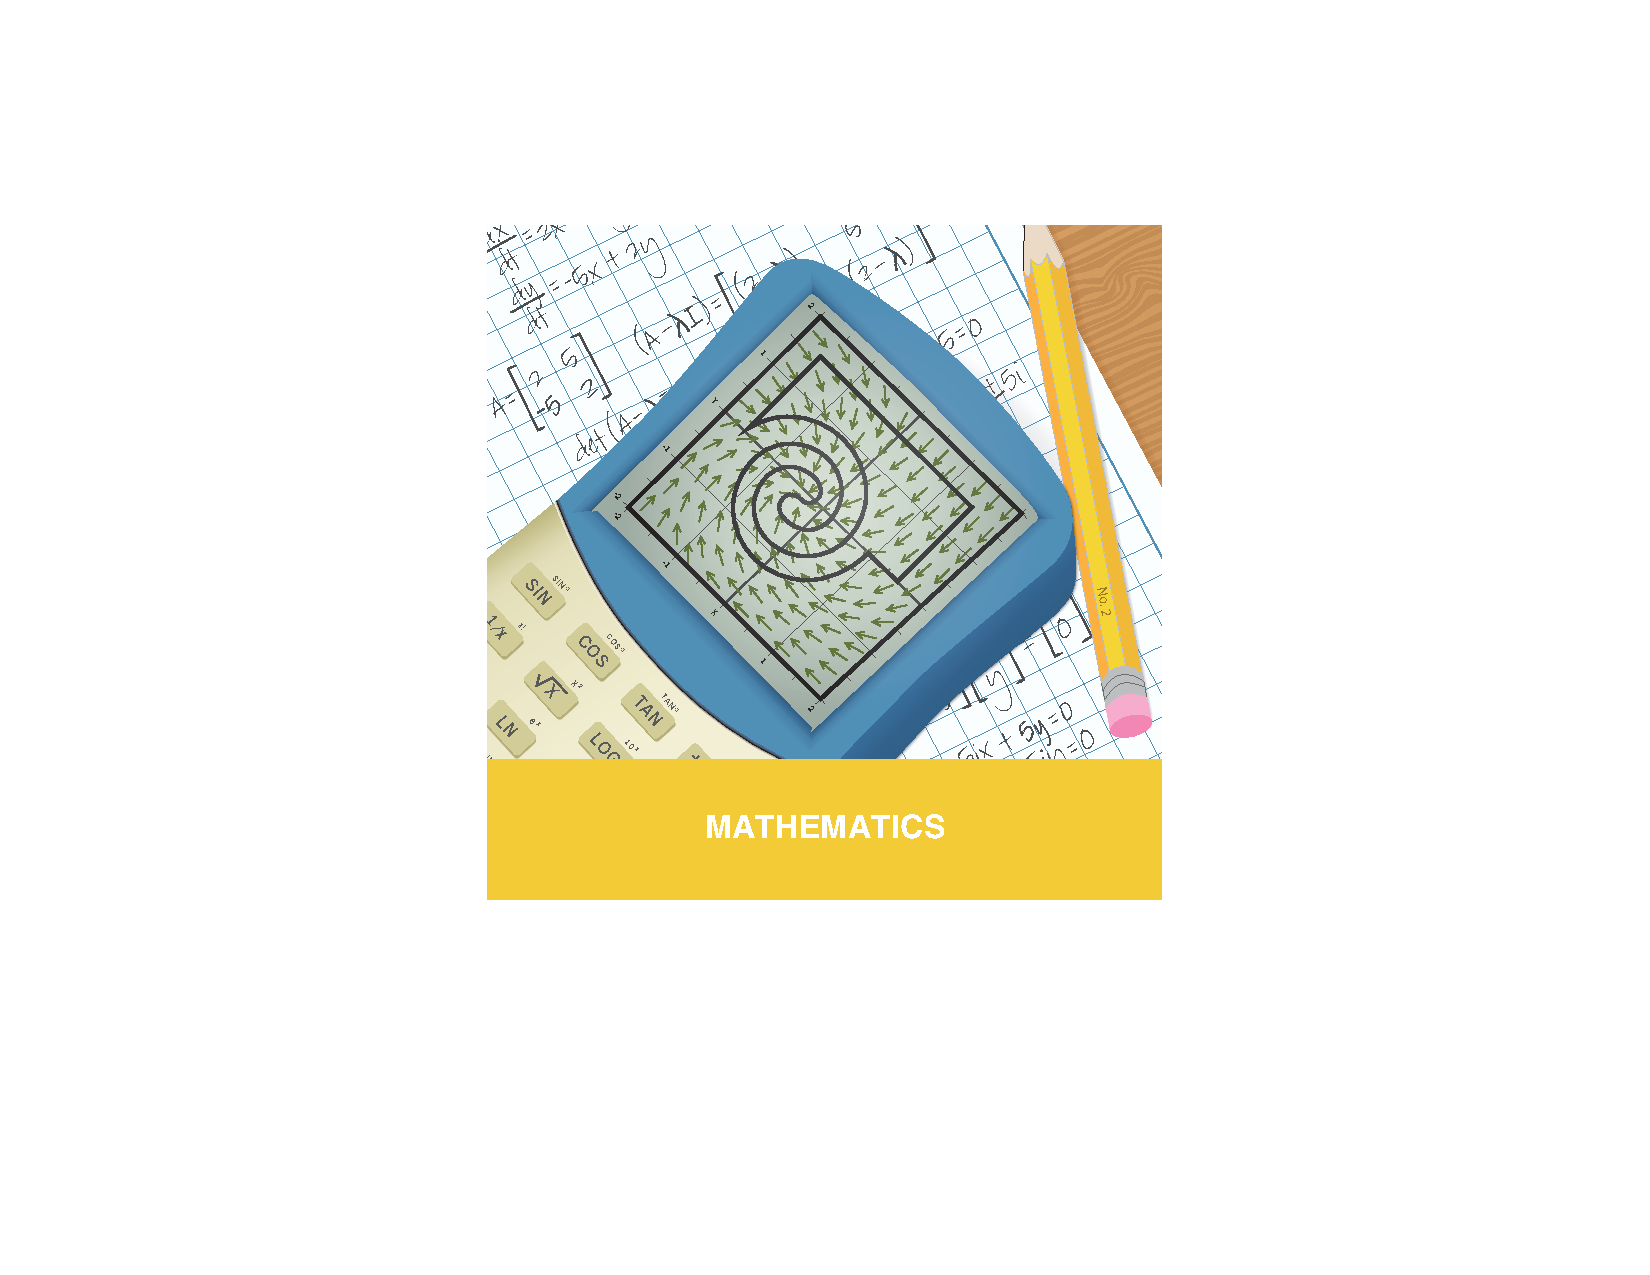
\includegraphics[width=\textwidth]{./50th_mathematicsproof}}

% from the titlesec package
%\titleformat{ command }
%             [ shape ]
%             { format }{ label }{ sep }{ before-code }[ after-code ]
% custom chapter
\titleformat{\chapter}
{\normalfont\Large\filleft\bf}                          % format applied to label+text
{}                                                      % label
{1pc}                                                   % horizontal separation between label and title body
{\resizebox{2cm}{!}{\color{gray!80}\thechapter}\\\Huge} % before the title body
[]                                                      % after the title body

% \chapter*
\titleformat{name=\chapter,numberless}
{\normalfont\huge\bfseries}{}{-20pt}{\Huge}

% custom section
\titleformat{\section}
{\itshape}
{\llap{\vbox to 5pt{\hbox{\resizebox{1cm}{!}{\normalfont\thesection}}}\hskip 9pt}}
{0pt}
{}

% custom paragraph heading
\titleformat{\paragraph}[leftmargin]
{\normalfont
\scshape\filleft}
{}
{0pt}
{}

% spacing around headings
% From the titlesec package
% \titlespacing{command}{left spacing}{before spacing}{after spacing}[right]
% spacing: how to read {12pt plus 4pt minus 2pt}
%           12pt is what we would like the spacing to be
%           plus 4pt means that TeX can stretch it by at most 4pt
%           minus 2pt means that TeX can shrink it by at most 2pt
%       This is one example of the concept of, 'glue', in TeX
\titlespacing{\chapter}{0pt}{0pt}{0.1cm}
\titlespacing\section{0pt}{12pt plus 4pt minus 2pt}{5pt plus 2pt minus 2pt}
\titlespacing\subsection{0pt}{12pt plus 4pt minus 2pt}{-6pt plus 2pt minus 2pt}
\titlespacing{\paragraph}{4pc}{1.5ex plus .1ex minus .2ex}{1pc}

% secnumdepth dictates which headings get enumerated- setting it 
% to 1 means that chapters and sections get enumerated, but 
% no headings below them will (such as subsection, subsubsection, paragraph, etc)
\setcounter{secnumdepth}{1}

% headers and footers
\fancyhf{} % delete current header and footer
\fancyhead[LE,RO]{\bfseries\thepage}
\fancyhead[LO,RE]{\leftmark}
\pagestyle{fancy}

% remove the word Chapter from the header
\def\chaptermark#1{\markboth{\textsc{\thechapter. \  #1}}{}}

%%% make refcheck and cleveref play nicely together: 
% http://tex.stackexchange.com/questions/87610/making-refcheck-work-with-cleveref
\makeatletter
\newcommand{\refcheckize}[1]{%
  \expandafter\let\csname @@\string#1\endcsname#1%
  \expandafter\DeclareRobustCommand\csname relax\string#1\endcsname[1]{%
    \csname @@\string#1\endcsname{##1}\wrtusdrf{##1}}%
  \expandafter\let\expandafter#1\csname relax\string#1\endcsname
}
\makeatother
% Now we add the reference commands we want refcheck to be aware of
\refcheckize{\cref}
\refcheckize{\Cref}
%%%

% wide page for side by side figures, tables, etc
\newlength{\offsetpage}
\setlength{\offsetpage}{3.0cm}
\newenvironment{widepage}{\begin{adjustwidth}{-\offsetpage}{-\offsetpage}%
                            \addtolength{\textwidth}{2\offsetpage}}%
                         {\end{adjustwidth}}

%\includeonly{OtherCurricularIssues}

\begin{document}

% The following lines should be uncommented in the final (production) version
%\maketitle
%\tableofcontents
%\printglossary

%= == == == == == == == == == == =
% main chapters
%= == == == == == == == == == == =
\renewcommand{\thesection}{\Alph{section}}
% arara: pdflatex: {files: [MathSACpr2014]}
\chapter{Other  Curricular Issues}\label{chap:otherissues}
\epigraph{Education is the only business still debating the usefulness of technology.}{Rod Paige, former U.S. Secretary of Education (2002)}
\section[Distance education]{To what degree are courses offered in a Distance
modality (online, hybrid, interactive television, etc)? For courses offered
both via DL and on-campus, are there differences in student success? (Contact
the Office of Institutional Effectiveness, either Laura Massey or Rob Vergun,
for course-level data). If so, how are you, or will you address these
differences? What significant revelations, concerns or questions arise in the
area of DL delivery?}\label{other:sec:distancelearning}

\subsection{Presence of DL offerings}
The Math SAC offers Distance Learning (DL) courses in online, hybrid, and
interactive television (ITV) modalities.  We strive to make our DL course
experience simulate the face-to-face course experience with respect to
instructor presence, feedback, and assessment. We use discussion boards to
simulate the classroom learning environment, and an array of online homework
platforms to assess and prepare our students effectively. A Math SAC DL standing
committee is charged with discussing the structure of our current DL courses, as
well as developing and maintaining current DL best practices and standards.

All of our pre-college level math courses (except a calculator skills course)
have a DL offering, as do most of our lower-division collegiate courses.
Courses that are not offered using a distance modality fall into two categories:
those on the high end of our collegiate courses, and specialty courses with low
enrollments; \cref{tab:sec3:DLofferings} shows complete details.

\begin{table}
\caption{Course Offerings through Distance Learning}\label{tab:sec3:DLofferings}
\centering
\begin{tabular}{ccccccccc}
\toprule
\multicolumn{3}{p{1in}}{Offered as DL} & \multicolumn{3}{p{1in}}{Not offered  DL upper division} & \multicolumn{3}{p{1in}}{Not offered  DL specialty}\\
\midrule
020& 030& 060& 		251& 252& 253&		015& 25C& 26C\\
065& 070& 084& 		254& 256& 261&		061& 062& 063\\
095& 111& 112& 		&&&					093& 105& 211\\
241& 243& 244&		&&&					212& 213\\
\bottomrule
\end{tabular}
\end{table}

Approximately 14.1\% of PCC math enrollments were DL based during the
academic year 2012/13 compared to only 9.1\% in the 2007/08 academic year.
This percentage increase is coupled with a general enrollment surge over the
past five years, and the number of DL enrollments has grown by over 150\% in
this time period. \Cref{fig:sec3:DLenrollments,fig:sec3:F2Fenrollments} show
student enrollment in face-to-face courses compared to online courses over six
academic years. Note that even while overall enrollment has declined some since
its peak in 2011/12, that absolute enrollment in DL courses has still grown.
\Cref{tab:sec3:F2FandDLdata2007,tab:sec3:F2FandDLdata2010} give more detailed data---note that we do not offer classes above MTH 244 in a DL modality.

\begin{figure}[!htb]
    \begin{minipage}{.5\textwidth}
          %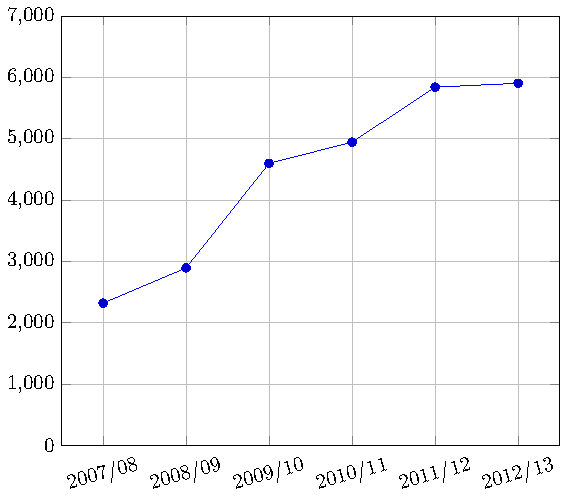
\includegraphics[width=\textwidth]{graphics/enrollmentInDL.pdf}
          % arara: pdflatex
% !arara: indent: {overwrite: yes}
\documentclass{standalone}
% Caption: Enrollment in DL
% 2007/08-2012/13

\usepackage{pgfplots}
\usepackage{pgfplotstable}
\pgfplotsset{compat=newest}


\begin{document}

% http://tex.stackexchange.com/questions/128468/problems-with-pgfplotstableread-and-relative-paths
\IfStandalone{
	\newcommand{\fromRoot}[1]{../data/#1}
	}{
	\newcommand{\fromRoot}[1]{./data/#1}
}

% need to have the read command in the main document, otherwise it will 
% be ignored when used with standalone
\pgfplotstableread[col sep=comma]{\fromRoot{ProcessedGradesData.csv}}\enrollmentdata

\begin{tikzpicture}
	\begin{axis}[
			%ybar,
			symbolic x coords={2007/08, 2008/09, 2009/10, 2010/11, 2011/12, 2012/13, NaN},
			xtick=data,
			minor ytick={1000,2000,...,7000},
			enlarge x limits,
			%scale only axis,       
			grid = both,
			ymin=0,ymax=7000,
			scaled ticks=false, 
			tick label style={/pgf/number format/fixed},
			legend pos=outer north east,
			restrict x to domain=0:5,
			x tick label style={rotate=25},
			width=\textwidth,
		]
		\addplot table[x=AY,y=DL_Enrollments]{\enrollmentdata};
		%\legend{DL}
	\end{axis}
\end{tikzpicture}
\end{document}

          \caption{Enrollments in DL}\label{fig:sec3:DLenrollments}
    \end{minipage}%
    \begin{minipage}{.5\textwidth}
          %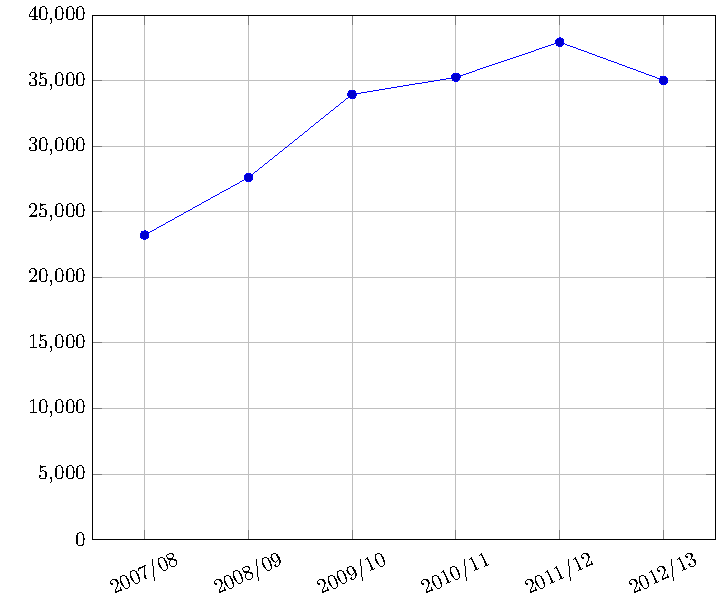
\includegraphics[width=\textwidth]{graphics/enrollmentInF2F.pdf}
          % arara: pdflatex
% !arara: indent: {overwrite: yes}
\documentclass{standalone}
% Caption: Enrollment in F2F
% 2007/08-2012/13

\usepackage{pgfplots}
\usepackage{pgfplotstable}
\pgfplotsset{compat=newest}

\pgfplotstableread[col sep=comma]{../data/ProcessedGradesData.csv}\enrollmentdata

\begin{document}

\begin{tikzpicture}
	\begin{axis}[
			%ybar,
			symbolic x coords={2007/08, 2008/09, 2009/10, 2010/11, 2011/12, 2012/13, NaN},
			xtick=data,
			%minor ytick={1000,5000,...,40000},
			enlarge x limits,
			scale only axis,       
			grid = both,
			ymin=0,ymax=40000,
			scaled ticks=false, 
			tick label style={/pgf/number format/fixed},
			legend pos=outer north east,
			restrict x to domain=0:5,
			x tick label style={rotate=15},
		]
		\addplot table[x=AY,y=F2F_Enrollments]{\enrollmentdata};
		%\legend{DL}
	\end{axis}
\end{tikzpicture}
\end{document}

          \caption{Enrollments in face-to-face classes}\label{fig:sec3:F2Fenrollments}
    \end{minipage}
\end{figure}

\begin{table}[!htb]
	\begin{widepage}
	\centering
  	\caption{DL \& Face-to-face (F2F) enrollments and pass rates 2007--2010}
    \label{tab:sec3:F2FandDLdata2007}
          % arara: pdflatex
\documentclass[varwidth]{standalone}
\usepackage{pgfplotstable}
\usepackage{booktabs}
\usepackage{multirow}

% caption: pass rates by class for DL vs F2F 2007-2008

% empty column type- very useful
\newcolumntype{H}{>{\setbox0=\hbox\bgroup}c<{\egroup}@{}}

\pgfplotstableset{percentstyle/.style={
    preproc/expr={##1*100},
    dec sep align,fixed,fixed zerofill,
postproc cell content/.append code={
            \ifx\\##1\\% check if ##1 is empty
            \else
            \ifnum1=\pgfplotstablepartno
                \pgfkeysalso{@cell content/.add={}{\,\%}}%
            \fi
            \fi
        },
    precision=0,
}
}

% references:
%   http://tex.stackexchange.com/questions/65760/pgfplotstable-how-can-i-add-percent-signs-and-respect-dec-sep-align
%   http://tex.stackexchange.com/questions/16604/easiest-way-to-delete-a-column/16607#16607
%   http://tex.stackexchange.com/questions/89365/check-for-empty-macro-argument

\begin{document}

% http://tex.stackexchange.com/questions/128468/problems-with-pgfplotstableread-and-relative-paths
\IfStandalone{
	\newcommand{\fromRoot}[1]{../data/#1}
	}{
	\newcommand{\fromRoot}[1]{./data/#1}
}

\pgfplotstableread[col sep=comma]{\fromRoot{dlvsF2FenrollmentPassRates.csv}}\dlvsftofdata

\pgfplotstabletypeset[
every head row/.style={
        before row={%
        \toprule
        \multirow{2}{*}{Course}
        & \multicolumn{7}{c}{2007--2008} 
        & \multicolumn{7}{c}{2008--2009} 
        & \multicolumn{22}{c}{2009--2010} 
        \\},
        after row=\midrule},
every last row/.style={after row=\bottomrule},
columns/Course/.style={string type,column name={},column type=r},
    % 2007-08
    % 2007-08
    % 2007-08
    columns/2007-08/.style={column type=H},
    columns/DL2007-08/.style={column name={DL},column type=r},
    columns/DL Pass rate2007-08/.style={column name={\% Pass},percentstyle},
    columns/FtoF2007-08/.style={column name={F2F},column type=r},
    columns/FtoF Pass rate2007-08/.style={column name={\% Pass},percentstyle},
    % 2008-09
    % 2008-09
    % 2008-09
    columns/2008-09/.style={column type=H},
    columns/DL2008-09/.style={column name={DL},column type=r},
    columns/DL Pass rate2008-09/.style={column name={\% Pass},percentstyle},
    columns/FtoF2008-09/.style={column name={F2F},column type=r},
    columns/FtoF Pass rate2008-09/.style={column name={\% Pass},percentstyle},
    % 2009-10
    % 2009-10
    % 2009-10
    columns/2009-10/.style={column type=H},
    columns/DL2009-10/.style={column name={DL},column type=r},
    columns/DL Pass rate2009-10/.style={column name={\% Pass},percentstyle},
    columns/FtoF2009-10/.style={column name={F2F},column type=r},
    columns/FtoF Pass rate2009-10/.style={column name={\% Pass},percentstyle},
    % 2010-11
    % 2010-11
    % 2010-11
    columns/2010-11/.style={column type=H},
    columns/DL2010-11/.style={column type=H},
    columns/DL Pass rate2010-11/.style={column type=H},
    columns/FtoF2010-11/.style={column type=H},
    columns/FtoF Pass rate2010-11/.style={column type=H},
    % 2011-12
    % 2011-12
    % 2011-12
    columns/2011-12/.style={column type=H},
    columns/DL2011-12/.style={column type=H},
    columns/DL Pass rate2011-12/.style={column type=H},
    columns/FtoF2011-12/.style={column type=H},
    columns/FtoF Pass rate2011-12/.style={column type=H},
    % 2012-13
    % 2012-13
    % 2012-13
    columns/2012-13/.style={column type=H},
    columns/DL2012-13/.style={column type=H},
    columns/DL Pass rate2012-13/.style={column type=H},
    columns/FtoF2012-13/.style={column type=H},
    columns/FtoF Pass rate2012-13/.style={column type=H},
    % ignore these columns
    columns/2008-09/.style={column type=H},
    columns/2009-10/.style={column type=H},
    columns/2010-11/.style={column type=H},
    columns/2011-12/.style={column type=H},
    columns/2012-13/.style={column type=H},
]{\dlvsftofdata}

\end{document}

          \vspace{2pc}
  	\caption{DL \& Face-to-face (F2F) enrollments and pass rates 2010--2013}
    \label{tab:sec3:F2FandDLdata2010}
          % arara: pdflatex
\documentclass[varwidth]{standalone}
\usepackage{pgfplotstable}
\usepackage{booktabs}
\usepackage{multirow}

% caption: pass rates by class for DL vs F2F 2010-2013

% empty column type- very useful
\newcolumntype{H}{>{\setbox0=\hbox\bgroup}c<{\egroup}@{}}

\pgfplotstableset{percentstyle/.style={
    preproc/expr={##1*100},
    dec sep align,fixed,fixed zerofill,
postproc cell content/.append code={
            \ifx\\##1\\% check if ##1 is empty
            \else
            \ifnum1=\pgfplotstablepartno
                \pgfkeysalso{@cell content/.add={}{\,\%}}%
            \fi
            \fi
        },
    precision=0,
}
}

% references:
%   http://tex.stackexchange.com/questions/65760/pgfplotstable-how-can-i-add-percent-signs-and-respect-dec-sep-align
%   http://tex.stackexchange.com/questions/16604/easiest-way-to-delete-a-column/16607#16607
%   http://tex.stackexchange.com/questions/89365/check-for-empty-macro-argument

\begin{document}

% http://tex.stackexchange.com/questions/128468/problems-with-pgfplotstableread-and-relative-paths
\IfStandalone{
	\newcommand{\fromRoot}[1]{../data/#1}
	}{
	\newcommand{\fromRoot}[1]{./data/#1}
}

\pgfplotstableread[col sep=comma]{\fromRoot{dlvsF2FenrollmentPassRates.csv}}\dlvsftofdata


\pgfplotstabletypeset[
every head row/.style={
        before row={%
        \toprule
        \multirow{2}{*}{Course}
        & \multicolumn{22}{c}{2010--2011} 
        & \multicolumn{7}{c}{2011--2012} 
        & \multicolumn{7}{c}{2012--2013} 
        \\},
        after row=\midrule},
every last row/.style={after row=\bottomrule},
columns/Course/.style={string type,column name={},column type=r},
    % 2007-08
    % 2007-08
    % 2007-08
    columns/2007-08/.style={column type=H},
    columns/DL2007-08/.style={column type=H},
    columns/DL Pass rate2007-08/.style={column type=H},
    columns/FtoF2007-08/.style={column type=H},
    columns/FtoF Pass rate2007-08/.style={column type=H},
    % 2008-09
    % 2008-09
    % 2008-09
    columns/2008-09/.style={column type=H},
    columns/DL2008-09/.style={column type=H},
    columns/DL Pass rate2008-09/.style={column type=H},
    columns/FtoF2008-09/.style={column type=H},
    columns/FtoF Pass rate2008-09/.style={column type=H},
    % 2009-10
    % 2009-10
    % 2009-10
    columns/2009-10/.style={column type=H},
    columns/DL2009-10/.style={column type=H},
    columns/DL Pass rate2009-10/.style={column type=H},
    columns/FtoF2009-10/.style={column type=H},
    columns/FtoF Pass rate2009-10/.style={column type=H},
    % 2010-11
    % 2010-11
    % 2010-11
    columns/2010-11/.style={column type=H},
    columns/DL2010-11/.style={column name={DL},column type=r},
    columns/DL Pass rate2010-11/.style={column name={\% Pass},percentstyle},
    columns/FtoF2010-11/.style={column name={F2F},column type=r},
    columns/FtoF Pass rate2010-11/.style={column name={\% Pass},percentstyle},
    % 2011-12
    % 2011-12
    % 2011-12
    columns/2011-12/.style={column type=H},
    columns/DL2011-12/.style={column name={DL},column type=r},
    columns/DL Pass rate2011-12/.style={column name={\% Pass},percentstyle},
    columns/FtoF2011-12/.style={column name={F2F},column type=r},
    columns/FtoF Pass rate2011-12/.style={column name={\% Pass},percentstyle},
    % 2012-13
    % 2012-13
    % 2012-13
    columns/2012-13/.style={column type=H},
    columns/DL2012-13/.style={column name={DL},column type=r},
    columns/DL Pass rate2012-13/.style={column name={\% Pass},percentstyle},
    columns/FtoF2012-13/.style={column name={F2F},column type=r},
    columns/FtoF Pass rate2012-13/.style={column name={\% Pass},percentstyle},
    % ignore these columns
    columns/2008-09/.style={column type=H},
    columns/2009-10/.style={column type=H},
    columns/2010-11/.style={column type=H},
    columns/2011-12/.style={column type=H},
    columns/2012-13/.style={column type=H},
]{\dlvsftofdata}

\end{document}

          \end{widepage}
\end{table}

As enrollment demand for DL math courses has increased, we have increased the
number of sections that we offer and trained more interested faculty in managing
DL courses.  Between the academic years of 2003/04 and 2007/08, the annual
number of sections offered increased from 51 to 87.  In the 2012/13 academic
year, we offered 185 DL sections.   The resulting increase in sections offers
access to students that can succeed in this modality and need this option due to
outside constraints such as work and family.


\subsection{Success rates in DL courses}
Pass rates in DL courses are quite noticeably lower than those for their
face-to-face counterparts. \Cref{fig:sec3:F2FandDLpassRates} visualizes the
difference in pass rates between the highest enrollment DL courses that we offer
and their face-to-face counterparts. More detailed data for all DL offerings can
be seen in \cref{tab:sec3:F2FandDLdata2007,tab:sec3:F2FandDLdata2010}. We recognize that students need a
certain level of self-discipline, better study skills, and comfort engaging with
technology to succeed in a DL course. However we currently have no method for
screening which students are less likely to succeed using a distance modality;
our recommendations on \cpageref{other:sec:recommendations} attempt to address this issue.


Referencing \cref{fig:sec3:F2FandDLpassRates}, 
it is clear that, in the six academic years shown, the pass rates 
generally decrease regardless of delivery mode.  We hypothesize that this
overall trend is mostly the result of the economic collapse of 2008 which led to
increased enrollment and changes in our student demographics (see demographics
data in \vref{app:sec:demographicdata}).  But the pass rates in DL courses are
as much as 30\% lower than in face-to-face counterparts and this large
discrepancy needs to be addressed.

\begin{figure}[!htb]
  \begin{widepage}
    \begin{subfigure}{.3\textwidth}
          % arara: pdflatex
% !arara: indent: {overwrite: yes}
\documentclass{standalone}
% Caption: Enrollment in DL
% 2007/08-2012/13

\usepackage{pgfplots}
\usepackage{pgfplotstable}
\pgfplotsset{compat=newest}

\pgfplotstableread[col sep=comma]{../data/ProcessedGradesData.csv}\enrollmentdata

\begin{document}

\begin{tikzpicture}
	\begin{axis}[
			%ybar,
			symbolic x coords={2007/08, 2008/09, 2009/10, 2010/11, 2011/12, 2012/13, NaN},
			xtick=data,
			%minor ytick={1000,2000,...,7000},
			enlarge x limits,
			scale only axis,       
			grid = both,
			ymin=0.3,ymax=0.85,
			axis y discontinuity=crunch,
			scaled ticks=false, 
			tick label style={/pgf/number format/fixed},
			legend pos=outer north east,
			restrict x to domain=0:5,
			x tick label style={rotate=15},
		]
		\addplot table[x=AY,y=020_DL_Pass_Rate]{\enrollmentdata};
		\addplot table[x=AY,y=020_F2F_Pass_Rate]{\enrollmentdata};
		\legend{DL 020, F2F 020}
	\end{axis}
\end{tikzpicture}
\end{document}

          \captionof{figure}{MTH 20}
    \end{subfigure}%
    \begin{subfigure}{.3\textwidth}
          % arara: pdflatex
% !arara: indent: {overwrite: yes}
\documentclass{standalone}
% Caption: Enrollment in DL
% 2007/08-2012/13

\usepackage{pgfplots}
\usepackage{pgfplotstable}
\pgfplotsset{compat=newest}

\pgfplotstableread[col sep=comma]{../data/ProcessedGradesData.csv}\enrollmentdata

\begin{document}

\begin{tikzpicture}
	\begin{axis}[
			%ybar,
			symbolic x coords={2007/08, 2008/09, 2009/10, 2010/11, 2011/12, 2012/13, NaN},
			xtick=data,
			%minor ytick={1000,2000,...,7000},
			enlarge x limits,
			scale only axis,       
			grid = both,
			ymin=0.3,ymax=0.85,
			axis y discontinuity=crunch,
			scaled ticks=false, 
			tick label style={/pgf/number format/fixed},
			legend pos=outer north east,
			restrict x to domain=0:5,
			x tick label style={rotate=15},
		]
		\addplot table[x=AY,y=060_DL_Pass_Rate]{\enrollmentdata};
		\addplot table[x=AY,y=060_F2F_Pass_Rate]{\enrollmentdata};
		\legend{DL 060, F2F 060}
	\end{axis}
\end{tikzpicture}
\end{document}

          \captionof{figure}{MTH 60}
    \end{subfigure}%
    \begin{subfigure}{.3\textwidth}
          % arara: pdflatex
% !arara: indent: {overwrite: yes}
\documentclass{standalone}
% Caption: Enrollment in DL
% 2007/08-2012/13

\usepackage{pgfplots}
\usepackage{pgfplotstable}
\pgfplotsset{compat=newest}


\begin{document}

% http://tex.stackexchange.com/questions/128468/problems-with-pgfplotstableread-and-relative-paths
\IfStandalone{
	\newcommand{\fromRoot}[1]{../data/#1}
	}{
	\newcommand{\fromRoot}[1]{./data/#1}
}
\pgfplotstableread[col sep=comma]{\fromRoot{ProcessedGradesData.csv}}\enrollmentdata

\begin{tikzpicture}
	\begin{axis}[
			%ybar,
			symbolic x coords={2007/08, 2008/09, 2009/10, 2010/11, 2011/12, 2012/13, NaN},
			xtick=data,
			%minor ytick={1000,2000,...,7000},
			enlarge x limits,
			%scale only axis,       
			grid = both,
			ymin=0.3,ymax=0.85,
			axis y discontinuity=crunch,
			scaled ticks=false, 
			tick label style={/pgf/number format/fixed},
			legend pos=south west,
			restrict x to domain=0:5,
			x tick label style={rotate=25},
            width=\textwidth,
		]
		\addplot table[x=AY,y=065_DL_Pass_Rate]{\enrollmentdata};
		\addplot table[x=AY,y=065_F2F_Pass_Rate]{\enrollmentdata};
		\legend{DL 065, F2F 065}
	\end{axis}
\end{tikzpicture}
\end{document}

          \captionof{figure}{MTH 65}
    \end{subfigure}

\vspace{2pc}

    \begin{subfigure}{.3\textwidth}
          % arara: pdflatex
% !arara: indent: {overwrite: yes}
\documentclass{standalone}
% Caption: Enrollment in DL
% 2007/08-2012/13

\usepackage{pgfplots}
\usepackage{pgfplotstable}
\pgfplotsset{compat=newest}


\begin{document}
% http://tex.stackexchange.com/questions/128468/problems-with-pgfplotstableread-and-relative-paths
\IfStandalone{
	\newcommand{\fromRoot}[1]{../data/#1}
	}{
	\newcommand{\fromRoot}[1]{./data/#1}
}
\pgfplotstableread[col sep=comma]{\fromRoot{ProcessedGradesData.csv}}\enrollmentdata

\begin{tikzpicture}
	\begin{axis}[
			%ybar,
			symbolic x coords={2007/08, 2008/09, 2009/10, 2010/11, 2011/12, 2012/13, NaN},
			xtick=data,
			%minor ytick={1000,2000,...,7000},
			enlarge x limits,
			%scale only axis,       
			grid = both,
			ymin=0.3,ymax=0.85,
			axis y discontinuity=crunch,
			scaled ticks=false, 
			tick label style={/pgf/number format/fixed},
			legend pos=north east,
			restrict x to domain=0:5,
			x tick label style={rotate=25},
            width=\textwidth,
		]
		\addplot table[x=AY,y=095_DL_Pass_Rate]{\enrollmentdata};
		\addplot table[x=AY,y=095_F2F_Pass_Rate]{\enrollmentdata};
		\legend{DL 095, F2F 095}
	\end{axis}
\end{tikzpicture}
\end{document}

          \captionof{figure}{MTH 95}
    \end{subfigure}%
    \begin{subfigure}{.3\textwidth}
          % arara: pdflatex
% !arara: indent: {overwrite: yes}
\documentclass{standalone}
% Caption: Enrollment in DL
% 2007/08-2012/13

\usepackage{pgfplots}
\usepackage{pgfplotstable}
\pgfplotsset{compat=newest}

\pgfplotstableread[col sep=comma]{../data/ProcessedGradesData.csv}\enrollmentdata

\begin{document}

\begin{tikzpicture}
	\begin{axis}[
			%ybar,
			symbolic x coords={2007/08, 2008/09, 2009/10, 2010/11, 2011/12, 2012/13, NaN},
			xtick=data,
			%minor ytick={1000,2000,...,7000},
			enlarge x limits,
			scale only axis,       
			grid = both,
			ymin=0.3,ymax=0.85,
			axis y discontinuity=crunch,
			scaled ticks=false, 
			tick label style={/pgf/number format/fixed},
			legend pos=outer north east,
			restrict x to domain=0:5,
			x tick label style={rotate=15},
		]
		\addplot table[x=AY,y=111_DL_Pass_Rate]{\enrollmentdata};
		\addplot table[x=AY,y=111_F2F_Pass_Rate]{\enrollmentdata};
		\legend{DL 111, F2F 111}
	\end{axis}
\end{tikzpicture}
\end{document}

          \captionof{figure}{MTH 111}
    \end{subfigure}%
    \begin{subfigure}{.3\textwidth}
          % arara: pdflatex
% !arara: indent: {overwrite: yes}
\documentclass{standalone}
% Caption: Enrollment in DL
% 2007/08-2012/13

\usepackage{pgfplots}
\usepackage{pgfplotstable}
\pgfplotsset{compat=newest}

\pgfplotstableread[col sep=comma]{../data/ProcessedGradesData.csv}\enrollmentdata

\begin{document}

\begin{tikzpicture}
	\begin{axis}[
			%ybar,
			symbolic x coords={2007/08, 2008/09, 2009/10, 2010/11, 2011/12, 2012/13, NaN},
			xtick=data,
			%minor ytick={1000,2000,...,7000},
			enlarge x limits,
			scale only axis,       
			grid = both,
			ymin=0.3,ymax=0.85,
			axis y discontinuity=crunch,
			scaled ticks=false, 
			tick label style={/pgf/number format/fixed},
			legend pos=outer north east,
			restrict x to domain=0:5,
			x tick label style={rotate=15},
		]
		\addplot table[x=AY,y=243_DL_Pass_Rate]{\enrollmentdata};
		\addplot table[x=AY,y=243_F2F_Pass_Rate]{\enrollmentdata};
		\legend{DL 243, F2F 243}
	\end{axis}
\end{tikzpicture}
\end{document}

          \captionof{figure}{MTH 243}
    \end{subfigure}
    \caption{Pass Rates By Modality}
    \label{fig:sec3:F2FandDLpassRates}
  \end{widepage}
\end{figure}

The difference in student-success rates between on-campus courses and DL courses
is an important issue for the Math SAC.  The Distance Learning Standing
Committee has met to consider this issue and the factors that lead to this
difference in success rates.  We can only speculate the reason for the disparity
based on anecdotal evidence and professional experience.  Students may no longer
see DL courses as unusual, so they may be unaware that successful DL math
students should have stronger study skills, self-discipline, and time management
skills than face-to-face math students absolutely need to be successful. We
believe that many students register for DL math courses without adequate
understanding of the study habits, time commitment, learning styles, and
technical skills that are necessary for success in these classes. Anecdotal
evidence suggests that some students who are aware of these issues and who would
otherwise enroll in a face-to-face section still enroll in a DL section due to a
lack of space in face-to-face sections.

There is currently a DL orientation available for DL students, but there is no
requirement that students complete it. Furthermore, there is no information in
the orientation to help students understand the particular challenges of
studying \emph{mathematics} using the DL delivery methods.  In many disciplines,
reading, writing, and discussion can be sufficient for learning. Students in
mathematics typically do not learn best until they have also acted, by working
through exercises or active problem-solving. In face-to-face classes,
instructors can monitor that this learning-through-action is happening more
easily. In DL courses, there is more of a need for students to rely on
self-discipline to complete this portion of their learning, and this is not
communicated in the existing DL orientation.


\subsection{Informing DL students}
The Course Information Page (CIP) is accessible to students registering for DL
courses and is meant to give section-specific information to students as they
decide which sections to register for.   Many faculty members use this system to
inform students of issues related to an online mathematics course.  For example,
faculty address the misconception that a DL class requires fewer hours of
attention per week than a face-to-face class. We believe that many students do
not visit the CIP for DL classes and continue to be unaware of the tools they
will need to be successful in a DL mathematics course.   Some faculty members
send emails to registered students before the term starts, asking them to read
the CIP;  it is not clear, however, how many students read this email or act on
it.  The link to a CIP is only available via the online class, and not via
MyPCC; this lack of presence may contribute to the issue.

Other methods that are employed by DL faculty to directly communicate with their
students include:
\begin{itemize}
\item using the Course Progress Notifications (CPNs);
\item placing telephone calls to students;
\item using Collaborate to hold online office hours in a kind of visual and aural chat session.
\end{itemize}

\subsection{Online homework platforms}
Faculty have sought to increase engagement by DL students through use of online
homework platforms. An online homework platform can provide students with
immediate feedback and also hold the student accountable for completion of
assigned exercises. Faculty can monitor progress and employ formative assessment
from a distance.

The SAC recognizes that program changes should come from research toward best
practices.  Faculty members Wendy Fresh, Rebecca Ross, Tammy Louie, Jessica
Bernards, and Diane Edwards have investigated the effects of use of an online
homework system in several experiments in both DL and face-to-face courses. In most
cases, results from these experiments suggest there may be positive effects to
using an online platform, but it remains too early to declare statistical
significance. To demonstrate statistical significance in studies of this nature
requires considerably large sample sizes. 

However Jessica Bernards has been able to measure one positive effect to a
significant degree. Instructor Bernards taught several online sections of MTH
111, with control groups doing homework from the textbook and submitting paper
write-ups, and experimental groups using online homework. The withdrawal rate
was 32\% for the control group and only 16\% for the experimental group, and
this difference was statistically significant ($P<1\%$).  Instructor Wendy Fresh
ran a very similar experiment with online sections of MTH 60. There may still be
an effect at that level, but more data is necessary to confirm with statistical
significance. Both instructors noted modest improvement in exam scores among the
experimental group, but again more data is being gathered to confirm with
significance.

For more information on research by Instructors Bernards and Fresh for DL
courses, see \vref{app:sec:onlinehwstudy}. For information on research by
instructors Edwards and Louie, see \vref{app:sec:aleks} and also
\cpageref{sec3:subset:alekspilot}. Research on the efficacy of WeBWorK (an online
homework platform discussed on \cpageref{other:sec:webwork}) was done in
\cite{focuswebwork}.  In \cite{brewer} it was found that when students are
segregated by incoming ability, those who were less prepared when entering a
course do benefit significantly from online homework use. As a community
college, we have more under prepared students than universities, so this
finding suggests that use of online homework may be more helpful at PCC. It is
important to note that each of these studies were done with face-to-face
courses; in DL courses the traditional homework alternative presents the
challenge of delivery, complicating the question in favor of using online
homework.

\subsection{WeBWorK}\label{other:sec:webwork}
Recent exciting developments at PCC have centered around the free and
open-source online homework platform called WeBWorK that is partially funded by
the National Science Foundation and maintained by the Mathematical Association
of America. By Spring 2014 we expect that over 20 faculty will be using WeBWorK
in their courses. The math SAC is also loaning out the services of Alex Jordan
to CTE and LDC science SACs to create free online homework review programs. We
envision using WeBWorK for future Learning Assessment research and placement
advising. We are working with Dual Credit instructors to offer WeBWorK services
to Portland Public Schools.

Most of the textbooks currently in use by the Math SAC are published by Pearson
Publishing, which offers MyMathLab for its online homework platform. While
MyMathLab and similar commercial products come as a bundled expense with new
textbook purchases, a separate online account for pairing with a used textbook
purchase is rather expensive. For this reason, face-to-face instructors rarely
require MyMathLab in their courses. On the other hand, Distance Learning
instructors have a stronger need for an online homework platform and the
majority of DL instructors do require that students use (and pay for) MyMathLab.

By contrast, WeBWorK is a platform for online homework that is free and
open-source. As there is no central headquarters for WeBWorK, it must be
installed on a server somewhere. Since joining the Math SAC in Spring 2009,
Alex Jordan has championed the implementation and use of WeBWorK at PCC. Some
PCC math faculty have used WeBWorK in various capacities by borrowing server
space from the University of Oregon, a relationship formed and maintained by
Jordan. This partnership between two Oregon state institutions has been
mutually beneficial. While PCC gained server access, PCC faculty members were
programming content that the University of Oregon has been able to take advantage of. Each term since
Fall 2011, roughly 10 sections of PCC math courses have used the UO server.

Over this period, WeBWorK users in the Math SAC lobbied Technology Solution
Services to provide the Math SAC with its own WeBWorK server. While the UO
server provided service to us, it came with certain restrictions and
complications that prevented WeBWorK at PCC from reaching its full potential.
For a time there was a chicken-and-egg situation, as TSS requested a greater
usage by PCC faculty before arranging for a server while some faculty chose not
to use WeBWorK because of the inconvenience of using the UO server.

In the 2012/13 academic year, faculty Chris Hughes and Scot Leavitt researched
accessibility issues (in the ADA sense) alongside Disability Services. See
\cite{accessibilityproject} for the full report. Among many other findings, they
found that MyMathLab (at the time of the project) had many significant
accessibility problems while WeBWorK was quite close to being fully ADA
compliant. The open-source nature of WeBWorK meant that the few remaining
obstacles to accessibility could be addressed. They recommended that the SAC
cease using MyMathLab for newly developed courses and newly developed online
shells. They also recommended that faculty migrate from MyMathLab to WeBWorK.
Disability Services supported their recommendations, and also began lobbying TSS
for a PCC WeBWorK server. Within the WeBWorK community PCC is now seen as a
leader when it comes to accessibility issues. See \cite{webworkblog} for a post
about this on the WeBWorK news blog. As a result of this, PCC is hosting a
WeBWorK development camp in August 2014 with a central theme of addressing
accessibility issues and enhancing its accessibility.\label{other:page:disabilityservices}

TSS partnered with the Clackamas Education Service District to deliver a WeBWorK
server that has been fully implemented since Winter 2014.  SAC members Alex Jordan,
Chris Hughes, and Xiaolong Yao have prepared
\href{http://webwork.pcc.edu}{webwork.pcc.edu} for regular use starting Winter
2014 term. A backup server at
\href{http://webwork-dev.pcc.edu}{webwork-dev.pcc.edu} is in place for faculty
to experiment with. 

The arrival of our own WeBWorK installation has significant implications beyond
homework management, particularly in the advising department. We envisage that
advisors would enroll students in a `review course' that contains (mostly)
pre-college practice problems, and that the student would be encouraged to sit
the COMPASS placement test only when they are comfortable with the problems in
WeBWorK. Furthermore, we can easily use WeBWorK as an advising tool to replace
Hughes' Placement Advisory Test (\cite{mathprogramreview2003}, pages 12--13) in situations when students are not happy with
their placement from COMPASS.  The SAC should work with advising to implement
this. 

\subsection{PCC WeBWorK problem library}
WeBWorK has been in use at universities for some time now, and an extensive
library exists of math problems for college-level courses. However there was
weak content support for basic algebra and other pre-college topics. Over Summer 2013, Alex Jordan, Chris Hughes, and Xiaolong Yao oversaw an effort to create
a library of high-quality, algorithmically generated, basic algebra WeBWorK
exercises which was partly funded with an IIP development grant; they received
support from math instructors Kandace Kling, Debbie Neft, Jeremy Shaw, and Danielle Rice.  These
exercises currently cover topics from MTH 60 and 65, and the team continues to
add problems to the library for MTH 95. The library development was a success
because of the strong collaboration and dedication of the three faculty members,
and the foundations that Jordan had laid in previous years. Jordan, Hughes,
and Yao presented their work at the STEM showcase (Rock Creek) in Fall 2013 (see
\cref{webworkposter}). It was at this showcase that the idea was hatched to
create free online homework review programs for CTE and LDC science SACs.

\begin{figure}[!htb]
	\centering
	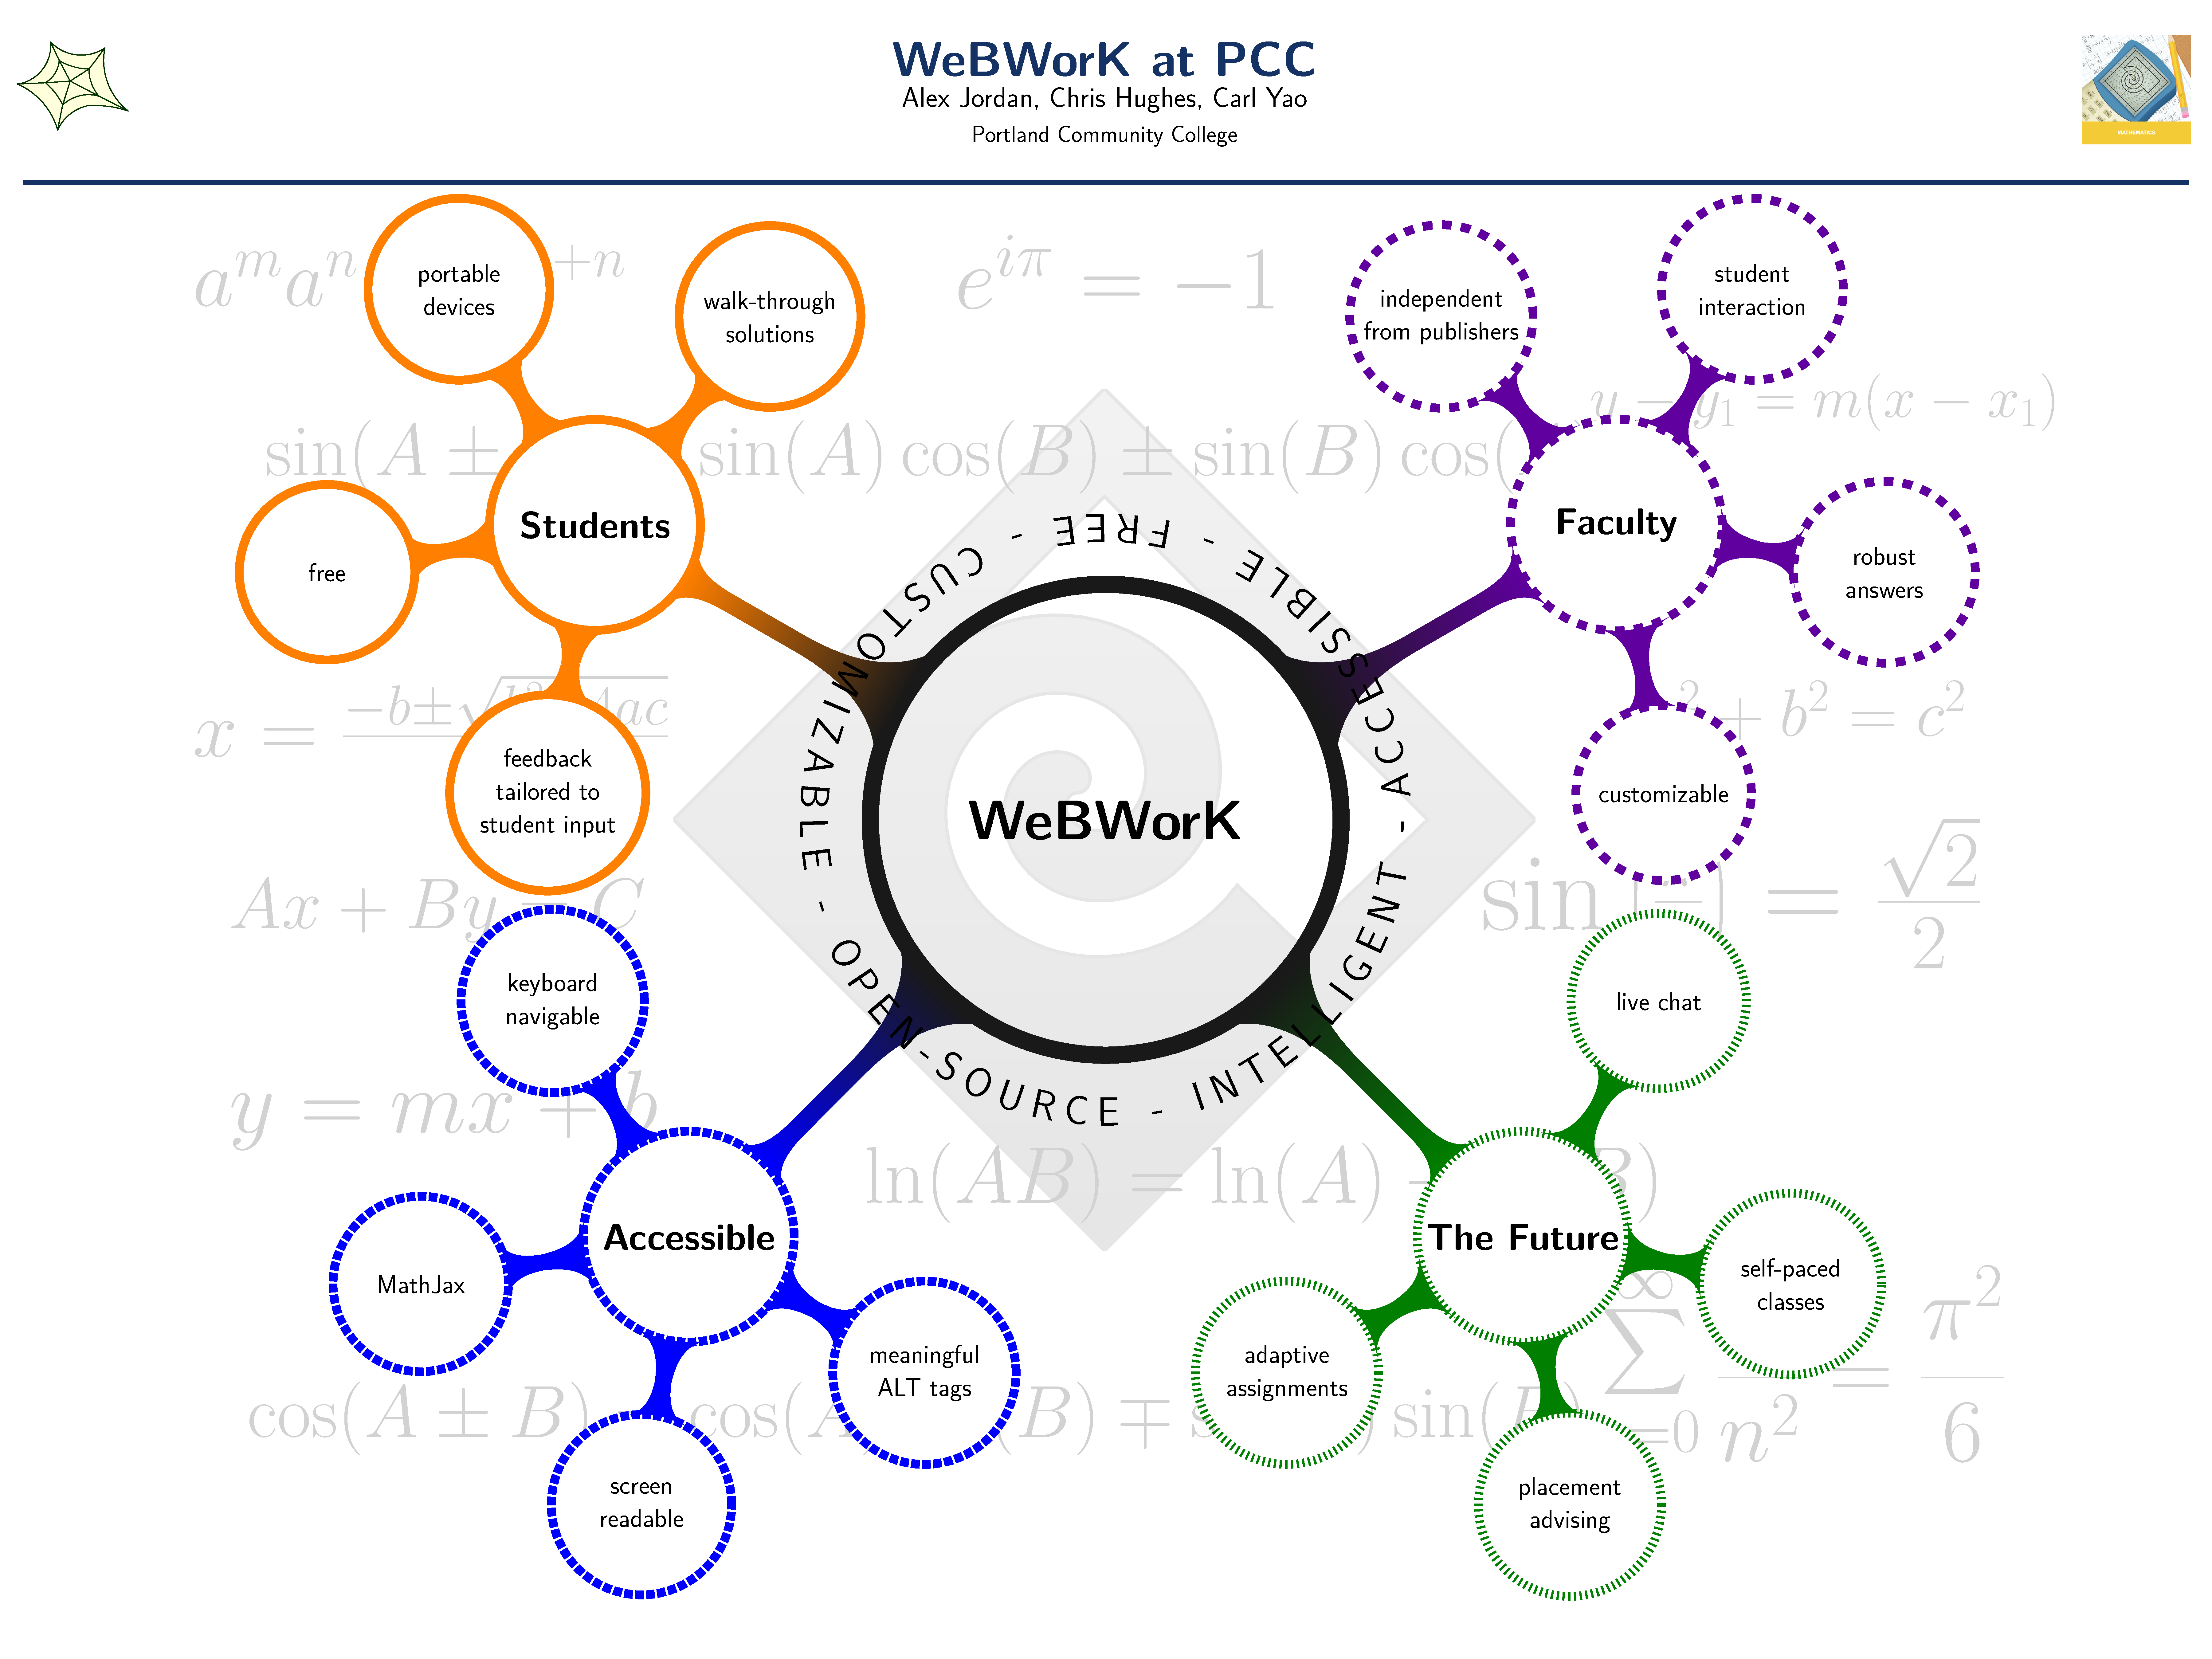
\includegraphics[width=0.5\textwidth]{webworkposter.pdf}
	\caption{WeBWorK poster from the PCC STEM Showcase}\label{webworkposter}
\end{figure}

As time and funding progress, SAC members with the requisite coding experience
hope to add more problems to this PCC library, expanding into the arenas of MTH
courses 20, 111, 112, 243, and 244. It is important to note the level of quality
of the problems from this library. Each problem has a full walk-through solution
coded along side the question which can be put to use by faculty in a number of
ways. Each problem is given fine attention to detail so that automated feedback
messages to the students are as informative as modern technology can allow. This
high level of quality requires time and experience to achieve. However it is
necessary if any instructor hopes to use WeBWorK as a teaching tool and not just
an assessment tool.

\subsection{Concerns about DL offerings}
Each of the following three issues have been raised by SAC members, and during
the 2012/13 academic year a group of concerned faculty met to discuss them. The
meetings were informal and no binding decisions were reached.
\begin{itemize}
\item Faculty are concerned about whether or not Distance Learning is an
  effective way to deliver math content, especially in light of the low pass
  rate statistics seen in \cref{fig:sec3:F2FandDLpassRates}. Successfully
  learning mathematics generally requires heavy active engagement. Face-to-face
  courses facilitate this engagement by requiring students to be in the physical
  presence of their instructor and fellow students. In DL courses, the
  imperative to remain engaged must come mostly from the student's own sense of
  responsibility and interest.
\item Faculty are concerned about the quality and consistency of current DL
  courses. Some faculty rely on publisher content such as electronic versions of
  textbooks, while other faculty have created complete sets of online notes
  themselves and use e-books only as secondary resources. Instructor Chris
  Hughes serves as an advisor to online faculty creating new courses, and makes
  recommendations to improve course quality and observe accessibility standards.
  However there is no enforcement of the online advisor's recommendations.
\item Faculty are concerned about the portion of a student's grade that may be
  computed from online homework. Compared to traditional homework, online
  homework is more readily vulnerable to cheating. With many math exercises, the
  exercise can literally be typed in to Google and the search engine itself
  provides an answer. Online homework provides fewer obstacles for a dishonest
  student to employ someone else to do their homework for them. In fact, in
  Craigslist sites nationwide, all one need do is search for `mymathlab' to find
  advertisements from those who will `take your online math course for you' at a
  cost. The math SAC has always wanted its online courses to mirror its
  face-to-face courses, and as a consequence has never created CCOGs that treat
  face-to-face and online courses differently. This has made it difficult to
  place any cap on the portion of a grade that may be computed from online
  homework. There is also no consensus on what an appropriate cap would be.
\end{itemize}

\subsection{Recommendations}\label{other:sec:recommendations}
\recommendation{Our main recommendations concern how to best inform students about the
particular skills that a distance learning student should have or adopt in order
to be successful. We also recommend enacting some prerequisite items for DL
registration to help give these skills to students. Lastly there are some
recommendations that do not fit these descriptions. Many of these
recommendations hold for face-to-face courses as well, and may be repeated elsewhere in
this program review.}
\begin{description}
\item For the Math SAC:
\begin{itemize}[label={}]
\item \recommendation{Collaborate with advising to implement a WeBWorK-based review mechanism
  for would-be placement test-takers.}
\item \recommendation{Consider how the quality of online courses could be improved by more effective regulation by the SAC. }
\end{itemize}
\item For Administration/Advising:
\begin{itemize}[label={}]
\item \recommendation{Collaborate with the Math SAC to implement a WeBWorK-based review
  mechanism for would-be placement test-takers.}
\item \recommendation{Give students more information on DL responsibilities and make students
  aware of the difference in student-success statistics between DL and face to
  face courses.}
\item \recommendation{Encourage students to contemplate why they seek to take a DL course and
  reflect upon whether it will align well with their learning style and
  personal skill sets.}
\end{itemize}
\item For Administration/DL/TSS:
\begin{itemize}[label={}]
\item \recommendation{Have the online orientation linked from the registration tool in MyPCC and
  require that students complete this orientation before registering for a DL
  class.}
\item \recommendation{Include a section in the DL orientation that addresses the specific
  challenges that DL brings to mathematics courses. Perhaps only students
  seeking to register for a mathematics DL course would be required to complete
  this section.}
\item \recommendation{Add redundant access to the Course Information Page. Along with access
  through the online Class Schedule, the CIP could be available through MyPCC on
  the home page for a course and through Desire To Learn.}
\item \recommendation{Include a pop-up or hover-over window that is activated when a student
  tries to register for a DL MTH class that gives specific information about the
  challenges of DL Math courses. }
\end{itemize}
\item For Administration/Other:
\begin{itemize}[label={}]
\item \recommendation{Require students to demonstrate pre-requisite computer literacy skills
  such as those taught in basic internet skills (CAS 104), beginning Word (CAS
  216), beginning keyboard (CAS 121), and basic computer skills/MS Office (CAS
  133).}
\item \recommendation{Develop and require a basic DL/computer skills competency course, possibly
  offered during week 0 of the term.  }
\item \recommendation{Provide opportunities for faculty professional development in research
  design and data analysis to help with research efforts on the efficacy of
  online homework.}
\item \recommendation{Provide support for further development of WeBWorK related projects,
  including a larger library of math problems for courses beyond 60/65/95,
  enhancements of the WeBWorK engine, and content for placement advising/review.}
\end{itemize}
\end{description}

\section[Curricular changes resulting from educational initiatives]{Has the SAC
made any curricular changes as a result of exploring/adopting educational
initiatives (e.g., Service Learning, Internationalization of the Curriculum,
Inquiry-Based Learning, Honors, etc.)?  If so, please describe.}


\subsection{Math 111H College Algebra: Honors}\label{cur:sub:111H}

The course has been offered only at Sylvania campus---Winter 2012 (12
students), Winter 2013 (22 students), Spring 2013 (15 students), and Fall 2013
(17 students).  Ronda Lively was the instructor the first three terms, which
allowed her to evolve her materials and activities.  Ann Cary taught the
Fall 2013 term, and has collaborated closely with Ronda Lively. 

The honors course must cover the same material as the regular course. It
is stressed that honors versions of a course should not be ``harder'', but
different in the use of class time and activities/assignments.  There should
also be a component of Community and Environmental Responsibility, which is a
PCC core outcome that is usually difficult to place in math courses.  Instructor
Lively regularly teaches MTH 111 and MTH 111H during the same term.  The same
exams were given in both courses.  There were differences in the other evaluation
criteria used in the courses.  In the MTH 111 class, students submitted take
home graded worksheets and participated in an in-class graded group activity.
The evaluation of the students in the MTH 111H class included:
\begin{itemize}
\item a collaborative computer project involving math history and investigation
  of several applications of math
\item a team quiz-grading activity where each group wrote a key and grading
  rubric, then applied it to two (fictional) students' quizzes
\item a community tutoring project:  over several weeks, each student found someone to
  tutor in math (friend, neighbor, family member, \ldots) and then wrote a paper
  on their experience
\end{itemize}
Since the overall student ability level was high, there was time in class to
investigate other topics of interest related to college algebra.  Each term
there were several students that enrolled because of the time slot,
not because they were strong in math.  Encouragingly, the
stronger students took the less prepared students under their wings and helped
them to be successful.


\subsection{Social justice workgroup}\label{cur:sub:socialJustic}
A Math and Social Justice workgroup was formed by Ann Cary and Emiliano Vega in
response to a national convention they attended. The group has collected and
disseminated data sets and activities to participating math instructors and has
gained interest and participants from other disciplines at PCC, as well as area
high school math instructors and community activists in Portland. More
importantly, the group has the focus of providing a forum on how to discuss
potentially sensitive subjects in a classroom setting when using application
problems and how to be more culturally and socially aware of individual students
and classes. The information they gathered has improved the pool of activities and application problems
available, improved the ability of instructors to work effectively with the
broad demographic of students and co-workers, and also continues the college's
focus on two Core Outcomes: Community and Environmental Responsibility and
Cultural Awareness. For a sample of material from this workgroup, see
\vref{app:sec:socialJustic}.

\subsection{Service learning}\label{other:sec:servicelearning}
Service Learning has been a part of many math instructors' courses at PCC, but
has been deepened through the Service Learning website
which includes additional resources and syllabi submitted
by participating Instructors at PCC. In addition, Service Learning will be
added to some CCOGs evaluation criteria to encourage instructors to incorporate
Service Learning in their math classes. Jeff Pettit participated as
an observer in the Service Learning training cohort at Sylvania campus,
connecting with instructors in other disciplines and gaining an understanding of 
how Service Learning is employed in other courses. This has led to new curriculum in his
Statistics courses and upper-division courses where Service Learning was not
originally employed.

\subsection{Developmental Education math study group}
A new committee was formed by the SAC to address developmental math completion
rates. The committee is researching the feasibility, cost and difficulty
associated with implementing ``pathways'' beyond the current calculus focused
MTH60--95 courses. The committee is considering options for employing
career-based math course series and a statistics-based math course series.

\subsection{Placement test reform group}\label{other:sec:placementreform}
A committee has been formed to address placement test reform. The
group intends to better measure students' needs beyond the current math-skills
COMPASS test. We hope to find a way to measure key traits and needs of students
to connect student populations with the support needed to better guarantee
success.
% I had encouraged these guys to work with student services, who are also
% addressing these concerns.  I don't know if they are or not though.  I do
% know that student services is working with the NSF Grant proposal team on
% these issues.  Perhaps a little more should be said here?

\section[Present dual credit relationships]{Are there any courses in the program
that are offered as Dual Credit at area High Schools?  If so, describe how 
the SAC develops and maintains relationships with the HS faculty in support of
quality instruction. Please note any best practices you have found, or ideas
about how to strengthen this interaction.  }

During the 2012/13 academic year, PCC dual credit was awarded
for seven mathematics courses.  Classes were offered at seven high schools and
there were a total of twelve instructors certified to teach PCC dual credit
mathematics classes.  There were a total of 750 unduplicated students who
enrolled in at least one PCC dual credit mathematics class and collectively
those students earned 6032 mathematics credits through PCC.
In Fall 2012, an ad hoc committee was formed in the mathematics SAC to investigate the status of our dual credit program.  The formation of this committee was prompted, in part, by the discovery that several of the posted dual credit syllabi described courses that bore little resemblance to the course for which students were earning PCC credit.  The committee decided that the root cause of this disconnect was a lack of robust support on our part.  Three concrete actions were taken to address the disconnect:
\begin{itemize}
\item Each dual credit mathematics instructor was assigned a team of two support
  faculty from the mathematics departments at PCC.  Each pair of support faculty
  visited their assigned instructor at that instructor's high school.  These
  meetings were rather informal; the intent being to establish a concrete
  support team for each high school instructor.
\item A two-day mandatory summer workshop was organized by the committee in
  conjunction with Beth Molenkamp, who at that time was the coordinator of
  PCC's dual credit program.  At the workshop each dual credit instructor was
  tasked to complete a robust (and accurate) syllabus for each of their dual
  credit classes.  The PCC faculty helped with this task and all of the dual
  credit instructors now have syllabi that truly reflect the nature of the
  course for which the students are earning PCC credit.  The remainder of the
  workshop was spent sharing resources and pedagogical tactics used by various
  PCC faculty in the courses for which dual credit is also offered.
\item A Google Drive site was created to share resources.  Although the
  inspiration for this site was to give our dual credit faculty easy access to
  shared resources, the pooling of resources is obviously of great benefit for
  PCC faculty as well.
\end{itemize}

\section[Future dual credit relationships]{Does the SAC plan to develop any
additional Dual Credit agreements with area high schools?  If so please
describe.   If not, what does the SAC see as barriers to developing further dual
credit agreements. }
Students at Central Catholic High School will get their first opportunity to
earn PCC mathematics dual credit during the 2013/14 academic year.  This
adoption was coordinated through the dual credit program; that is, the math SAC
played no active role in the creation of this dual credit agreement.

There is concern in the mathematics SAC that the state's 40-40-20 initiative,
and the accompanying bills aimed at encouraging high school students to earn
college credits, might lead to a dramatic increase in the number of high
schools offering dual credit for mathematics courses. The greatest challenge is
that there are not that many high school mathematics instructors who meet PCC's
qualifications to teach post-100 level mathematics courses.  We are concerned
that the day might come where we are pressured to lower those standards or, of
even more concern, we are pressured to start awarding PCC dual credit for
developmental mathematics courses (MTH 95 or below).

\subsubsection{Addendum}
As feared, we are now being asked to allow high school instructors who do not
satisfy minimum qualifications to teach transfer level courses.  As currently
proposed, the under-qualified high school instructor would be paired with an
``instructor of record'' who does meet the qualifications;  we are concerned by
this proposal on many levels.  

The first is fundamental: this proposal makes a
mockery of the phrase ``minimum qualifications.'' While we realize that the
pressure to make this change originates from the State of Oregon, we need to be
mindful that our accreditation is also at stake.  

Additionally, there are
fears that the concept will seep into the manner in which we staff classes on
our own campuses; an alternative minimum qualification such as ``demonstrated
competency'' cannot be exclusive to teachers in the high school classrooms.

Finally, if the concept takes off at the  dual credit level, there are serious
workload concerns for the faculty at PCC.  
The title of ``instructor of record''
comes with a serious amount of responsibility and accountability;  authentic
and ongoing involvement in these courses will require time from a faculty that
is already stretched for time.  We are presently being asked to revamp
our entire DE curriculum (and are actively involved in that pursuit), but  adding
increased dual credit involvement to our list of duties will take away time
from that agenda; priorities need to be established.  If the college chooses to
pursue this change in dual credit policy we hope that the changes are
instituted in a manageable and reputable way.

\section[Other significant curricular changes]{Identify and explain any other
significant curricular changes that have been made since the last
review.}\label{cur:sec:other}

\subsection{MTH 20 moved to the Math SAC from the DE SAC}
The MTH 20 curriculum was moved into the Math SAC from the DE SAC in Fall 2012,
bringing all math curriculum under the same SAC.  This move was meant to help
create consistency in the CCOGs across the spectrum of math courses, as well as
ensure that the MTH 20 curriculum is adequately preparing students for the next
math course.

Sylvania Campus, which had a separate DE Math department altogether,
transitioned its DE Math instructors into the Math Department in Fall 2013.  A
Math Integration Work Group was formed and charged with creating a seamless path
for this transition.  With the DE Math instructors in the Math SAC and the
current college focus on success in pre-college math courses, the Math SAC's focus is
on producing high-yield instructional practices, student success, and completion
across the span of math courses offered by the college.
 
\subsection{MTH 20 proposed credit change: 4- to 5-credit}\label{cur:sub:mth20}
MTH 20 (Basic Math) is a content-heavy course that covers topics such as
fractions, decimals, signed number operations, geometry, proportions, and
percents.  It can be argued that the amount of material covered in MTH 20 is
greater than in any of our other mathematics courses.  At times, instructors are
forced to either minimize required topics or occasionally cut them entirely due
to time constraints.  Because of this, for years many MTH 20 instructors have
wanted to increase the number of credits for the course.  

In October 2012, the SAC received a memo from the DOIs related to class sizes in
which we were encouraged to consider converting MTH 20 from 4- to 5-credits;  a subcommittee was formed by the SAC to investigate the benefits and
consequences of increasing the number of credits.  The committee
looked into the financial aid impact on students, the impact on
degree/certificate programs, and the impact on classroom availability.  It also
rewrote the CCOG to include study skills and increase the emphasis on reading
graphs and geometry in the course.  

In April 2013, the Mathematics SAC approved the conversion of MTH 20 from a
4-credit course to a 5-credit course.  The conversion was then approved by the
Curriculum Committee in November 2013.  Unfortunately, the current DOIs denied
the recommendation in late November 2013;  since the original recommendation came to
the Math SAC in 2012, the college leadership has changed at many levels, and
with these changes have come changes in perspectives and goals for the math
curriculum.
The Math SAC is currently engaged in reevaluating and reorganizing pre-college
level math at all levels; it is highly likely that the first course will
require 5 credits for optimal student success.

\subsection{MTH 60/65/70/95 curriculum alignment}
The Math SAC recognized that students successfully completing MTH 65 often had
difficulty passing MTH 95.  The same was true for students transitioning between
MTH 95 and MTH 111.

It was thought that creating more continuity between the MTH 60/65 series and
MTH 95 would improve student success.  To this end, during 2008/09, a committee
was created to redesign the 60/65/95 curriculum with an eye toward carefully
preparing students for the rigor of college level mathematics.  While MTH 60,
MTH 65 and MTH 95 had been traditionally taught as algebraically focused
classes, the committee adjusted the curriculum to reflect the need for students
to be able to understand mathematical information via the `rule of four':
algebraically, graphically, numerically and verbally.  This was done to prepare
students for the demands of college level math and to align with the best
practices of our field.  Importance was also placed on the use of a graphing
calculator in MTH 95 to aid in this.  These changes were also reflected in the
intermediary course in the MTH 60/65/95 series: MTH 70.
 
As with all curricular changes, there continues to be a need for ensuring that
all of the instructors receive the necessary communication and support in
implementing these changes.  This is especially true for the part-time
instructors who are teaching a large proportion of the MTH 60--95 courses.  However,
with the nature of the part-time instructor's working conditions, this continues
to be a challenge.  The Math SAC requests more support from the administration
to provide the necessary funding for part-time instructors to attend
course-specific meetings similar to the one held for MTH 95 instructors at the
Sylvania Campus prior to the Fall 2013 term.
 
\subsection{Replaced MTH 111A/111B/111C with MTH 105 and MTH 111}
In 1997 the Math SAC split MTH 111 into three courses in order to target
different student populations: MTH 111A for liberal art students, MTH 111B for
business and other non-technical majors, and MTH 111C for Science and
Engineering.  In our last Program Review, \cite{mathprogramreview2003}, 
it was mentioned that we eliminated MTH 111A and resurrected MTH 105 (see \cite{mathprogramreview2003} page 19).  
Since then, MTH 111B and 111C have merged again into MTH 111.  

The CCOGs for MTH 111B and MTH 111C had grown
increasingly similar; since both were prerequisites for the same courses
(MTH 243 and MTH 112), they needed to cover the same content.  MTH 111B had a
reputation for being an easier course and many instructors noticed that students
in MTH 112 who had taken MTH 111B instead of MTH 111C were less prepared.  Since
the two courses no longer served different purposes, and were creating problems 
with student preparation for subsequent courses, we decided to unify MTH 111B and MTH 111C into a single
college algebra course starting in Fall 2012: MTH 111.
 
\subsection{MTH 243 credit change: 4- to 5-credit}\label{other:sec:mth243}
The Math SAC increased credits for MTH 243 (Statistics I) from 4-credits to
5-credits for several reasons, most of which were related to a need to increase
the contact hours from four hours to five hours.  In order to address the needs
of future coursework in statistics as well as sufficient coverage of material
for transfer to many universities, it was essential to add more material to the
4-credit MTH 243 course.  Increasing the credit hours allowed for the necessary
contact time to cover such material appropriately.
 
 
Five contact hours allows for more integration of technology into the classroom,
since these technology skills are best learned with hands-on guidance from 
the instructor. Formerly, it
was often difficult to have meaningful technology-oriented statistical classroom
exercises due to the lack of contact time.
 
The change to five contact hours also gives sufficient time to fully engage the
students with critical thinking exercises and quantitative and statistical
literacy discussions.

\subsection[Creation of AMP/MTH008]{Creation of two accelerated review courses
(also referred to as the Accelerated Math Program, or AMP) MTH 07 and MTH 08}
\label{other:sec:amp} 
\begin{description}
\item[MTH 07: Accelerated Basic Math Review]  This course presents a review of
  basic math skills and provides the opportunity for guided practice.  Topics
  include operations with whole numbers, fractions, decimals, proportions and
  percents.

\item[MTH 08: Accelerated Introductory Algebra Review] This course presents a
  brief review of basic algebra skills and provides the opportunity for guided
  practice.  Topics include real number operations, manipulating linear
  expressions, solving linear equations, and graphing linear equations in two
  variables.
\end{description}

These two courses were designed to meet the needs of the following two student
populations:
\begin{itemize}
\item students who have previously learned the material and are able to test
  into the next level of math as a result of a brief review;
\item students who have difficulty with the materials and can work on a variety
  of the regular course material in advance of taking the regular course.
\end{itemize}

Both courses are offered for one week in-between terms and are 15 non-credit lab
hours.  They are taught with a combination of mini lectures and computer
practice/instruction.  At the completion of each course, students retake the
COMPASS placement test.  Each term a significant number of students taking these
courses have placed into a MTH course above their previous COMPASS placement.

Sections have been offered at the Rock Creek, Southeast, and Cascade Campuses,
with most offerings at the Cascade Campus, where the courses were initially conceived and implemented by math instructors Holli Adams and  Michael Marciniak. Data from the sections taught at
Cascade Campus since 2010 can be viewed in \vref{app:sec:ampdata}.
 
\subsection{Clarified CCOGs requirements and CCOG addendums}
It was found that there were numerous discrepancies among different sections of
the same course having different instructors regarding the material being
presented. In an effort to ensure that students completing different sections of
the same course had similar mathematical competencies, the SAC determined that
communicating the requirements for a course needed to be made more concise.
Also, since the curriculum had significantly changed, we wanted instructors who
had previously taught the course to know about these changes.  The CCOG for each
course was intentionally written more clearly and now includes specific minimum
requirements for testing and grading.  In addition, each CCOG now has an
addendum that clearly shows examples of what is expected in terms of content,
mathematical notation and presentation as well as well-defined assessment
strategies.  This practice has now been adopted for most of our CCOGs.
 
\subsection{Elimination of MTH 91 and MTH 92}
MTH 91 and MTH 92 were created to address the issue of the high failure rate in
MTH 95 by splitting up the content of MTH 95 into two terms.  The course
sequence was discontinued after data showed that students taking MTH 91 and 92
were not successful in the subsequent course, MTH 111; it was found that after
taking these slower paced classes, the students were not prepared for the speed
of the MTH 111 course.
 
\subsection{Changes in MTH 251--254}
The calculus series has been more strongly split into Calculus I/II and Calculus
III/IV by requesting the publisher split the current text into two sections.
This change altered the need for Maple in MTH 251 and MTH 252.  Maple is an
expensive graphing software package that students buy for one year but generally
use only for Calculus IV. Attaching Maple to the new second half of the book
solved the issue of students losing access to it if they took more than one year
to complete the Calculus series.

\subsection{Math study skills material development}\label{cur:sub:studyskills}
Research has shown that students with strong study skills are more successful in
their academic pursuits than their counterparts; however, many
students entering developmental mathematics courses lack these skills.
In an effort to help students build a stronger awareness of how a successful
student studies, math SAC member Jessica Bernards from the Rock Creek Campus
created a Math Study Skills program to be used in our developmental math
courses.  This program consists of seven topics all relating to study skills
specific to mathematics: how learning math is different, resources available for
help at PCC, time management, listening and note-taking skills, how to do
homework, test taking strategies, and overcoming math and test anxiety.  

Each lesson has three parts: a short video to be watched by students
outside of class, a student worksheet to be completed in conjunction with the
video, and an in-class discussion lead by the instructor. Additionally, each
topic has quotes from successful students which help strengthen the ideas in
each video.  Many math instructors across all campuses piloted the program in
the Spring 2013 and are continuing to use it this Fall 2013. For Winter 2014,
fourteen DE math instructors have reported that they will be using it. The study
skills website can be found at \cite{studyskills}.
 
\subsection{MTH 111/112 document project}\label{cur:sec:111/112doc}
In Winter 2010, Math SAC member Chris Hughes proposed that the SAC write its own
MTH 111/112 textbook. This idea arose from a general frustration with
commercially available textbooks for this sequence.  Available books tend to
fall on one end or another of a spectrum ranging from template-based and lacking
in conceptual understanding to abstract and lacking in guidance for students.
We seek something with better balance.  Such a 
textbook could also be provided to students at a much lower cost than any commercial 
product.

Initially over 10 members of the Math SAC became involved, submitting ideas and
small sections of what might someday become a textbook.  As time passed, four
SAC members (Chris Hughes, Alex Jordan, Ann Cary, and Steve Simonds) maintained
serious interest in the project.  Piecing together earlier work from the larger
group, expanding on that work, and editing, these four produced a rough draft
chapter representing about 10\% of a final product. (Given that this draft would
need editing, we estimate that it represents 5\% of the work necessary for
completion.)

At this point the four remaining editors put active work on hold until some level of
release time can be secured that would enable completion in a timely manner.  A
completed textbook for the entire sequence could be drafted with three faculty
taking one-third release time for two consecutive terms.  An additional such
term would provide for peripherals such as guided lecture notes, an online
homework library, and LiveScribe videos. The progress to date can be found at
\cite{mth111project}.
% Math 111 textbook, recommendations/request:  I hope that this is among your
% recommendations in chapter 6?
 
\subsection{Supplemental course packets}
Textbooks that the Math SAC selects for courses often have gaps when
compared to the CCOGs for that course.  Supplemental course packets were created
to fill in the gaps and are required for those specific classes.  These include
explanations of topics not covered in the textbook as well as example
problems to fully cover a topic that might be lacking in the textbook examples.
Supplemental course packets have been created for MTH 60, 65, 95, 111 and 112,
and can be (freely) downloaded from the Math department's web site
\cite{pccmathdept}.
 
\subsection{MTH 251 lab manual}
Since the late 1990s, MTH 251 has been taught in a lecture/lab format.  From
that time through the late 2000s the materials used during the lab portion of
the course were frequentyly modified.  By 2009 the lab manual had
devolved into a collection of random problems and there was simply no connection 
between one set of problems and the next; there also were limited central themes to any one set of problems.

In Summer 2009 faculty member Steve Simonds rewrote the lab manual from
scratch.  The problem sets were written in a deliberate way to help students
develop deep understanding of key concepts covered in the course.  The majority
of the problems from the prior lab manual were then shuttled to the appendix as
practice problems for outside of class.  All of the practice problems were fully
keyed so that the students could continue thinking about the ideas (and
practicing the skills) covered in lab and then determine for themselves if they
had come to reasonable conclusions.

\subsection{MTH 105 course material flexibility}
Each math course has traditionally used the same SAC approved textbook
district-wide.  The Math SAC broke from this tradition and voted to allow MTH
105 instructors to choose their own course material, provided it meets the
approval of the MTH 105 CCOG committee.  Unlike other math classes, MTH 105 is not a
prerequisite for other math courses, and is a terminal math course for many
of our students.  Each term, the instructor selects three to five topics from a
list of 17.  This allows the instructors flexibility to teach material
appropriate for the student population of each class.

\subsection{ALC math courses}
The ALC math courses are self-paced pre-college math courses\footnote{The Alternative
Learning Center (ALC) was an old name for the current Sylvania Student Learning Center.}.
They are designed for students to work independently at their own pace and allow
them to focus on specific topics.  Consequently, a wide range of students take
these courses: students who are afraid to take a math class and want to get back
into math slowly; students who failed a math class once or several times; students
who feel that they placed too low on the placement test and just need a review;
students who want to get through the material quickly; and international
students who know the math but not the English terminology for it.  At Sylvania,
the majority of students who take ALC Math are students who have failed math classes,
sometimes many times.

Historically, the ALC math courses have been offered at Sylvania Campus, housed
by the Developmental Education SAC, and covered math content through MTH 65.
Since Summer 2012, they have also been offered at Southeast Campus.  Since
Winter 2013, ALC is housed in the Math SAC and, since Fall 2013, it also
includes MTH 95. For a more thorough look at these changes see
\vref{app:sec:alc}. Considerations are currently being made to find ways to have
ALC Math at Cascade and Rock Creek.  Students from these campuses are
already using ALC Math at Sylvania and Southeast and are undergoing the hardship
of travel just so they can take these courses.

Enrollments at Sylvania and Southeast both show that there is clearly a need for
these courses.  Research done by PCC's Institutional Effectiveness on data from
five years at Sylvania shows that students who complete ALC Math successfully
pass their math classes at a higher rate than before taking ALC Math  (see
\vref{app:sec:effectivenessALC}).  It would therefore be well worth looking into
using the ALC math classes as an early intervention when students fail math classes.
At Sylvania, for instance, some
full-time advisors have made themselves very familiar with the ALC math courses and
suggest them to students early on.  Others send students to the Math Coordinator for
further advising regarding successfully completing math classes.
 
\subsection{MTH 84: Introduction to \LaTeX}\label{other:sec:mth84}
In Spring 2010, Math SAC members Alex Jordan and Chris Hughes proposed a pilot
course to teach the typesetting software \LaTeX.  The experimental, one-credit course was piloted for
three consecutive terms (Fall 2010, Winter 2011, and Spring 2011) and then
adopted by the SAC as MTH 84.  The course was first run (as MTH 84) in Winter
2012, and has run each term since with one section per term. MTH 84 is a one-credit 
pass/no-pass course. Its modality has been DL, although the CCOG does not
prevent a face-to-face version.  The course serves students and faculty alike in many areas.
\LaTeX\ is a useful tool in math, the sciences, in graphic design, and in
publishing; it can easily be used to typeset internal documents, such as Program Reviews.
 
\subsection{MTH 76 Math SAC approval}
The SAC approved the CCOG for a one-credit `Introduction to GeoGebra' course. The course is
planned to run as a pilot course in Spring 2014 and Summer 2014, with tentative
approval to let it run as a permanent course Fall 2014.  The audience for the
course includes PCC students, PCC instructors who wish to use it as a teaching
tool, and K--12 teachers who wish to use it as a teaching tool.  The course was
requested by high school teachers participating in the Dual Credit workshop in Summer 2013.

\subsection[ALEKS pilot]{Pilot using ALEKS technology in two math courses during AY 2012/13}\label{sec3:subset:alekspilot}
ALEKS technology requires students to complete each mathematics topic
successfully, keeps track of student work time, provides instant feedback,
routinely assesses students and requires them to revisit previously learned
material.  It allows students to study a variety of topics at a time and
minimizes practice of mastered material. Two pilots of ALEKS in MTH 20 and MTH
112 were conducted.

\begin{description}
\item[MTH 20: Basic Mathematics] ALEKS was incorporated into six online and six
  on-campus MTH 20 classes.  Data was compared to the previous year's MTH 20
  classes taught by the same two instructors, Diane Edwards and Marilyn
  Marshall.  On average, courses using ALEKS had noticeably higher pass rates
  than non-ALEKS courses.  For example, there was an 11\% increase in pass rates
  in on-campus ALEKS classes in Fall 2012 compared to non-ALEKS Fall 2011
  classes.  Both on-campus and DL classes showed increased passing rates using
  ALEKS.  In addition, a few students each term were able to complete two
  courses during one term, finishing Basic Mathematics early and then
  successfully completing MTH 60.

\item[MTH 112: Elementary Functions] ALEKS was incorporated into one Elementary
  Functions section and compared with two traditional sections, all taught by
  faculty member Tammy Louie.  In this small sample, both the grade distribution
  and pass rates were similar.  However the student retention rate in the ALEKS
  class was 17.3\% higher than in the non-ALEKS classes.  
 
 \end{description}
 
In both pilots students were observed to enjoy using ALEKS and increase their
study time while using ALEKS.  More detailed data can be found in the
\vref{app:sec:aleks} concerning both pilot projects. These pilots of ALEKS had
noticeable success with student perception and involvement.  Further
exploration of ALEKS technology should be pursued as a possible option to
improving student success in mathematics courses.
 
\subsection{MTH 112 formula sheet}
The SAC approved a standardized ``formula sheet'' for use in MTH 112.  Math SAC
member Wendy Fresh revised and submitted a formula sheet edited from one
provided by SAC member Pete Haberman.  The page was added to the course CCOGs to
help guide instructors and clarify evaluation expectations.
 
\subsection{MTH 212 proficiency exam}
With SAC approval, the MTH 211--213 instructors added a basic skills proficiency
exam to MTH 212 that must be passed with no less than a 90\% in order to pass
the course.  MTH 212 is the second of a three part series of courses for
students preparing to enter a teacher education field. The proficiency exam
covers basic operations on integers, fractions, decimals, and percents.
Although there is a MTH 95 prerequisite for the MTH 211--213 series, many of the
students do not remember these basic operations. Since these are topics covered
in MTH 212, it was felt that holding the students responsible for the basic
skills would help them grasp the concepts with more success.  This approach has
been adopted by several of the Oregon community colleges and four-year
universities that offer the MTH 211--213 sequence.

\subsection{Casio Classpad}
The SAC approved of the Casio Classpad as an additional accepted graphing
calculator in MTH 95 and Lower Division Transfer courses. In addition, the CCOG
for MTH 93, the one-credit graphing calculator class, was revised to reflect topics
specific to the Casio Classpad. Faculty members Tammy Louie and Alex Jordan
created a PCC-specific user guide for the Classpad, which is available for
download (along with earlier PCC calculator manuals) at the math department web
site \cite{pccmathdept}. 

\subsection{Piloting of DE courses geared to a specific subset of CTE students}
In 2009, Choul Wou, a Perkins advisor, asked Michele Marden collaborate with her to create a reference document to support CTE students in the Building Inspection, Interior Design, Architecture, and Drafting programs. There was a particular need to bridge from MTH 65 coursework to ARCH 122. Michele observed an ARCH 122 section and a document was created. Soon after, Michele was approved to teach two sections of MTH 60 and one section of MTH 65 reserved for CTE students in the programs stated above. The course focus was limited by the requirements of the CCOGs, but whenever possible, material was geared to support the mathematical needs for these programs. This experience lead to the awareness that the reference document needed significant revision; however, due to the development of CTE-focused courses, the reference document was not updated. The specialized courses were discontinued due to lack of enrollment.


%= == == == == == == == == == == =
% appendices
%= == == == == == == == == == == =
\appendix
% add the word Appendix to the header
\def\chaptermark#1{\markboth{\textsc{Appendix \thechapter. \  #1}}{}}
% custom section
\titleformat{\section}
{\Large\bfseries}
{\llap{\thesection\hskip.5cm}}
{0pt}
{}
\titlespacing\section{0pt}{12pt plus 4pt minus 2pt}{-5pt plus 2pt minus 2pt}

\renewcommand{\thesection}{\arabic{section}}
% start a partial tableofcontents for the appendix
%\chapter*{Appendices}
\addcontentsline{toc}{chapter}{Appendices}
\startcontents[appendixtoc]
%\printcontents[appendixtoc]{}{0}{}
% arara: pdflatex: {files: [MathSACpr2014]}
% !arara: indent: {overwrite: yes}
\chapter{Changes in ALC Math Courses}\label{app:sec:alc}
After MTH 20 was moved to the Math SAC, the ALC math courses were the only math courses left in the DE SAC. The ALC math instructors therefore requested that these courses too would be moved to the Math SAC. After the DE and Math SACs gave their support, the courses were moved in January 2013.

Historically, the ALC math courses have only included curriculum up to MTH 65, but after the move was completed, the Math SAC voted to also include MTH 95 curriculum from Fall 2013 on.

Furthermore, the ALC math courses have been impacted by the new no-repeat policy. Historically, these courses could be repeated many times because they included three math levels (now four). Since Winter 2014, each level has their own set of courses. Following is a listing  of the previous and the new/changed courses:

\begin{multicols}{2}
Previous courses (until Fall 2013):
\begin{itemize}[label={}]
  \item ALC 60 Basic Math Skills Lab
  \item ALC 61 Basic Math Skills Lab
  \item ALC 62 Basic Math Skills Lab
  \item ALC 63 Basic Math Skills Lab
\end{itemize}
\vfill
\columnbreak
New courses (since Winter 2014):
\begin{itemize}[label={}]
  \item ALC 20A Math 20 Lab - 0 credits 
  \item ALC 20B Math 20 Lab - 1 credit 
  \item ALC 20C Math 20 Lab - 2 credits 
  \item ALC 20D Math 20 Lab - 3 credits 

  \item ALC 60A Math 60 Lab - 0 credits 
  \item ALC 60B Math 60 Lab - 1 credit 
  \item ALC 60C Math 60 Lab - 2 credits 
  \item ALC 60D Math 60 Lab - 3 credits 

  \item ALC 65A Math 65 Lab - 0 credits 
  \item ALC 65B Math 65 Lab - 1 credit 
  \item ALC 65C Math 65 Lab - 2 credits 
  \item ALC 65D Math 65 Lab - 3 credits 

  \item ALC 95A Math 95 Lab - 0 credits 
  \item ALC 95B Math 95 Lab - 1 credit 
  \item ALC 95C Math 95 Lab - 2 credits 
  \item ALC 95D Math 95 Lab - 3 credits
\end{itemize}
\vfill
\end{multicols}

% arara: pdflatex: {files: [MathSACpr2014]}
% !arara: indent: {overwrite: yes}

\chapter{Core Outcomes Mapping}\label{sec:app:coreoutcomes}

\begin{minipage}[t]{.45\textwidth}
Mapping Level Indicators:
\begin{enumerate}
  \item Not Applicable.
  \item Limited demonstration or application of knowledge and skills.
  \item Basic demonstration and application of knowledge and skills.
  \item Demonstrated comprehension and is able to apply essential knowledge and skills.
  \item Demonstrates thorough, effective and/or sophisticated application of knowledge and skills.
\end{enumerate}
\end{minipage}\hfill
\begin{minipage}[t]{.45\textwidth}
Core Outcomes (CO): 
\begin{enumerate}
\item Communication.
\item Community and Environmental Responsibility.
\item Critical Thinking and Problem Solving.
\item Cultural Awareness.
\item Professional Competence.
\item Self-Reflection.
\end{enumerate}
\end{minipage}%

\pgfplotstableread{
	Course 	{Course Name}	CO1	CO2	CO3	CO4	CO5	CO6
	{MTH 10}	{Basic Math}	4	0	4	0	4	3
	{MTH 20}	{Basic Math}	4	0	4	0	4	3
	{MTH 30}	{Business Mathematics}	4	0	4	0	4	3
	{MTH 60}	{Introductory Algebra, 1st term}	4	0	4	0	4	3
	{MTH 61}	{Introductory Algebra, Part I}	4	0	4	0	4	3
	{MTH 62}	{Introductory Algebra, Part II}	4	0	4	0	4	3
	{MTH 63}	{Introductory Algebra, Part III}	4	0	4	0	4	3
	{MTH 65}	{Introductory Algebra, 2nd term}	4	0	4	0	4	3
	{MTH 70}	{Introduction to Intermediate Algebra}	4	0	4	0	4	3
	{MTH 91}	{Intermediate Algebra, Part I}	4	0	4	0	4	3
    {MTH 92}	{Intermediate Algebra, Part I}I	4	0	4	0	4	3
    {MTH 93}	{Intro to TI Graphics Calculator}	4	0	4	0	4	3
    {MTH 95}	{Intermediate Algebra}	4	0	4	0	4	3
    {MTH 111} 	{College Algebra}	4	0	4	0	4	3
    {MTH 112}	{Elementary Functions}	4	0	4	0	4	3
    {MTH 211}	{Foundations of Elementary Math I}	4	0	4	0	4	3
    {MTH 212}	{Foundations of Elementary Math II}	4	0	4	0	4	3
    {MTH 213}	{Foundations of Elementary Math III}	4	0	4	0	4	3
    {MTH 241}	{Calculus for Management}	4	0	4	0	4	3
    {MTH 243}	{Statistics I}	4	0	4	0	4	3
    {MTH 244}	{Statistics II}	4	0	4	0	4	3
    {MTH 251}	{Calculus I}	4	0	4	0	4	3
    {MTH 252}	{Calculus II}	4	0	4	0	4	3
    {MTH 253}	{Calculus III}	4	0	4	0	4	3
    {MTH 254}	{Calculus IV}	4	0	4	0	4	3
    {MTH 259}	{Single Variable Calculus Review}	4	0	4	0	4	3
    {MTH 256}	{Differential Equations}	4	0	4	0	4	3
    {MTH 261}	{Applied Linear Algebra}	4	0	4	0	4	3

	}\coreOutComes

\pgfplotstabletypeset[
begin table=\begin{longtable},
end table=\end{longtable},
	every head row/.style={
		before row=\toprule,
		after row=\midrule},
	every last row/.style={after row=\bottomrule},
    every row no 8/.style={after row=\cmidrule{2-8}},
    every row no 12/.style={after row=\cmidrule{2-8}},
    every row no 14/.style={after row=\cmidrule{2-8}},
    every row no 20/.style={after row=\cmidrule{2-8}},
	columns/Course/.style={string type,column type=l},
	columns/Course Name/.style={string type,column type=l},
]{\coreOutComes}

% arara: pdflatex: {files: [MathSACpr2014]}
% !arara: indent: {overwrite: yes}
\chapter{Course Scheduling Pattern (by campus)}\label{sec:app:courseschedule}
\section{Cascade}
\begin{enumerate}
    \item  Scheduling is term by term, which helps us adjust to enrollment
      changes and part-time faculty changes.
    \item  Class size for all Cascade math classes is capped at 35 (if room
      allows) except MTH 20/61/62/63, which are capped at 30.
    \item  Since the last program review, we have regularly offered many more
      MWF classes, especially for MTH 95, in order to try to improve retention
      and success.  MWF classes, meeting for shorter times than typical MW/TuTh
      classes, enable us to `pack' more classes into a school day and therefore
      maximize our usage of the rooms we are assigned.
    \item  We discontinued MTH 91/92 because we felt that the sequence was
      inadequately preparing students for MTH 111.
    \item We discontinued offering MTH 20 DL because student success rates were 
      lower than in the face-to-face format.
    \item  We continued to innovate with regard to hybrid offerings, including
      weekday and Saturday hybrids.
    \item  We eliminated Sunday hybrids when Cascade decided to eliminate
      Sunday class offerings.  Since we were beginning to see declines in
      enrollment anyway, this did not seriously impact student access to
      classes.  The Saturday hybrids are still available.
\end{enumerate}

\section{Rock Creek}
\begin{enumerate}
    \item Rock Creek schedules term by term.  It would help with staffing
      decisions if the classes would be assigned rooms well ahead of the date
      the class offerings become visible to students online and the deadline
      for the photograph proof of the paper class schedule.
    \item Rock Creek offers mostly two day a week classes (82\%) meeting from
      7am to 9  pm, about 10\% one day a week either Saturday or Friday
      mornings, and 8\% online.
    \item Rock Creek schedules courses at the Hillsboro Center, Willow Creek
      Center and St Helens  (12\% of class offerings at RC).
\end{enumerate}

\section{Sylvania}
\begin{enumerate}
    \item  Scheduling is done one year ahead, which helps students plan out
      their year.
    \item  Coordination between campuses for low enrollment or specialty
      courses.
    \item  Newberg Center, scheduled by Sylvania, gives more students better
      access.
    \item  Increased offering of Distance Learning courses also increases
      accessibility for students with scheduling conflicts.
	\item  Class size for all Sylvania math classes is capped at 34 (if room allows) except
    Statistics (23-28 for computer classrooms).
	\item  Reorganized the time slots for 2013/14 which should lower possibility of canceled classes (due 
	to room availability or low enrollment).
\end{enumerate}

\fixthis{why is SE not included here?}

% arara: pdflatex: {files: [MathSACpr2014] }
% !arara: indent: {overwrite: yes}
\chapter{DL survey summary}\label{app:sec:dlsurveysummary}
Survey data details: $n=976$ face to face and $n=291$ online responses.

\fixthis{are the verbal descriptions necessary here? are they included somewhere else?}
\begin{enumerate}
	\item Have you used any of the resources available through the library (e.g. calculator, netbook, or iPad rentals, textbook checkouts, scanners, or online database search engines) during your time as a student in a PCC math course?
	\begin{enumerate}
		\item     Yes. I frequently used these resources.
		\item    Yes, but I seldom/rarely used these resources.
		\item     No, but I knew that such resources were available.
		\item     No, and I was unaware that such resources were available.
	\end{enumerate}
	We found that our students both in face-to-face and online classes are generally knowledgeable about library and out of the classroom resources such as calculator rentals, netbook and iPad rentals, textbook checkouts, scanners and online searchable databases.
	\fixthis{should these tables be centered? or should we use tabularx to get them to fit the linewidth?}
		
	\begin{tabular}{lc}
		\toprule
		              & Student knowledge of library and out-of classroom resources \\
		\midrule
		Face-to-face  & $81.45\%$                                                   \\
		Online/hybrid & $74.25\%$                                                   \\
		\bottomrule
	\end{tabular}
	
	Not surprising that library and other out-of-the-classroom information is being used more frequently by our face-to-face students than that of online students. This could be due to less frequent visits to campus for online students and/or online students already have the resources available to them. 
	
	\begin{tabular}{lc}
		\toprule
		              & Actual use of library and out-of-classroom resources \\
		\midrule
		Face-to-face  & $48.76\%$                                            \\
		Online/hybrid & $25.77\%$                                            \\
		\bottomrule
	\end{tabular}
	\item Were the library and related resources listed on your most recent math course syllabus?
	\begin{enumerate}
		\item Yes, it is listed on the syllabus with links.
		\item Yes, it is mentioned but no links are provided.
		\item No, it is not listed as a resource.
		\item I don't have a copy of the syllabus available.
	\end{enumerate}
	We found that both Part-time faculty and Full-time faculty included information regarding library and out-of-classroom resources on their syllabi.
	
	\begin{tabular}{lc}
		\toprule
		                  & Percentage of classes where the syllabus included resources \\
		\midrule
		Part-time faculty & $69.41\%$                                                   \\
		Full-time faculty & $69.48\%$                                                   \\
		\bottomrule
	\end{tabular}
	
	The data suggests that there was very little distinction of which classes encourage more students to use outside resources in both our college level and pre-college level mathematics. 
	
	\begin{tabular}{lc}
		\toprule
		                  & Percentage of classes where the syllabus included resources \\
		\midrule
		College level     & $70.05\%$                                                   \\
		Pre-College level & $68.83\%$                                                   \\
		\bottomrule
	\end{tabular}
	\item Does your current math course have online homework and/or online assessments available (e.g. WeBWorK, MyStatLab, MyMathLab, ALEKS)?
	\begin{enumerate}
		\item Yes, it is required.
		\item Yes, but it is optional.
		\item No such resource is available.
	\end{enumerate}
	Online homework has grown in popularity over the past few years. There has been much debate within our SAC if students should be required to use online homework in face-to-face and online classes. The question has often been raised if students should be required to pay an extra cost for such features and if so, what is a reasonable cost to the student? The data shows a general trend that online homework programs such as Webwork,  MyMathLab, MyStatLab, and ALEKS are being used more frequently in online than face-to-face classes. 
	
	\begin{tabular}{lc}
		\toprule
		              & Percentage of classes requiring online homework \\
		\midrule
		Face-to-face  & $13.93\%$                                       \\
		Online/hybrid & $70.45\%$                                       \\
		\bottomrule
	\end{tabular}
	
	Data suggests that significantly more Full-time instructors are offering some form of online homework (either required or optional) than that of Part-time instructors. This discrepancy may reflect the need to convey and distribute more information about these programs should Part-time instructors want to offer similar options to their students.
	
	\begin{tabular}{lc}
		\toprule
		                  & Percentage of classes offering some form of online homework \\
		\midrule
		Full-time faculty & $70.78\%$                                                   \\
		Part-time faculty & $54.93\%$                                                   \\
		\bottomrule
	\end{tabular}
	\item I am willing to pay up to \$35 extra for access to online homework and resources that may help me succeed.
	\begin{enumerate}
		\item Strongly agree
		\item Agree
		\item Neutral
		\item Disagree
		\item Strongly disagree
	\end{enumerate}
	When asked if students would be willing to pay up to \$35 to access online homework and resources that may help them to succeed, we found that online students were more willing to pay an extra fee. It should be mentioned that we previously mentioned data that online students were more likely to have used online homework and hence be better equipped to compare cost versus benefit. In contrast, a student who has not been previously exposed to an online homework system may not be able to properly address possible benefits and instead answer purely based on willingness to pay the given dollar amount. 
	    
	\begin{tabular}{lc}
		\toprule
		              & Percentage of student willing to pay for online homework   \\
		\midrule
		Face-to-face  & $18.44\%$                                                  \\
		Online/hybrid & $42.61\%$                                                  \\
		\cmidrule{2-2}
		              & Percentage of student unwilling to pay for online homework \\
		\cmidrule{2-2}
		Face-to-face  & $56.86\%$                                                  \\
		Online/hybrid & $27.14\%$                                                  \\
		\bottomrule
	\end{tabular}
	
	Note that the above values do not include the students who responded “neutral” on the question as these differences were not statistically significant. 
	\item What Learning Management Software are available for your math course? Bubble in all that apply.
	\begin{enumerate}
		\item  Instructor web page
		\item  D2L and/or MyPCC
		\item  MyMathLab or MyStatLab
		\item  Other
		\item  None of the above
	\end{enumerate}
	\item Of the available Learning Management Software, which ones have you used? Bubble in all that apply.
	\begin{enumerate}
		\item  Instructor web page
		\item   D2L and/or MyPCC
		\item   MyMathLab or MyStatLab
		\item   Other
		\item   None of the above
	\end{enumerate}
	We found that a majority of our courses are using outside resources to connect with students. These resources include but are not limited to personal instructor websites, DesiretoLearn, MyPCC, MyMathLab, MyStatLab, etc. 
	
	\begin{tabular}{lc}
		\toprule
		              & Percentage of classes offering additional resources \\
		\midrule
		Face-to-face  & $89.75\%$                                           \\
		Online/hybrid & $99.31\%$                                           \\
		\bottomrule
	\end{tabular}
	
	A larger separation existed for Part-time instructors who do not use any of the above mentioned resources. This could be due to lack of information or lack of knowledge about available resources.
	
	\begin{tabular}{lc}
		\toprule
		                  & Percentage of classes offering additional resources \\
		\midrule
		Full-time faculty & $95.32\%$                                           \\
		Part-time faculty & $86.72\%$                                           \\
		\bottomrule
	\end{tabular}
	
	Overall MyMathLab and MyStatLab are used more frequently in pre-college level classes in contrast to college level classes. 
	
	\begin{tabular}{lc}
		\toprule
		                  & Percentage of classes offering MML or MSL \\
		\midrule
		College level     & $31.49\%$                                 \\
		Pre-College level & $48.54\%$                                 \\
		\bottomrule
	\end{tabular}
	
	\item What resources available from the PCC Math Department have you used? Bubble in all that apply.
	\begin{enumerate}
		\item  Course supplements
		\item  Calculator manuals
		\item  Math 251 Lab Manual
		\item  Other
		\item  None of the above
	\end{enumerate}
	Our math department website offers additional materials for students. This includes course specific supplements to the textbook, calculator manuals specific to PCC math courses, required Calculus 1 lab, and other information regarding course description. Students may print these materials for free from any PCC computer lab. 
	\item What graphing software programs have you used? Bubble in all that apply.
	\begin{enumerate}
		\item  WolframAlpha
		\item  Graph
		\item  WinPlot
		\item  Other (e.g. Fooplot, Maple, GeoGebra)
		\item  None of the above
	\end{enumerate}
    \fixthis{fix column alignment on next table using siunitx}
	
	\begin{tabular}{lc}
		\toprule
		                                     & Resources used by students in College Level Courses \\
		\midrule
		Wolfram Alpha                        & $24.88\%$                                           \\
		Graph                                & $14.90\%$                                           \\
		Winplot                              & $6.14\%$                                           \\
		Other (Maple, GeoGebra, FooPlot,etc) & $27.34\%$                                           \\
		None of the above                    & $51.77\%$                                           \\
		\bottomrule
	\end{tabular}
  \item Which of the following resources available at PCC have you used? Bubble all that apply.
    \begin{enumerate}
      \item  On-campus Student Learning Centers
      \item  Online tutoring
      \item  The Student Help Desk
      \item  Other (e.g. Collaborate or Elluminate)
      \item  None of the above
    \end{enumerate}
    We encourage students to use some of the resources that PCC offers such as On-campus Student Learning centers, online tutoring, student help desk, Collaborate and/or Elluminate. We found that a significant amount of students in Face-to-Face classes were using the resources whereas students enrolled in an online class were not.  This is not especially surprising since the nature of online courses allows infrequent campus visits for the student. However, we could work to encourage the use of online tutoring to our online demographic.

	\begin{tabular}{lc}
		\toprule
		              & Percentage of students using PCC learning resources\\
		\midrule
		Face-to-face  & $67.32\%$                                                   \\
		Online/hybrid & $36.08\%$                                                   \\
		\bottomrule
	\end{tabular}
  \item Which of the following resources do you use for your math class that is available outside of PCC?  Bubble all that apply.
    \begin{enumerate}
      \item Private Tutoring
      \item  Math websites  (such as Khan Academy, Purple Math, etc.)
      \item  Youtube videos not provided by instructor
      \item  Other
      \item  None of the above
    \end{enumerate}
With the wide-spread availability of the internet, students have been increasingly using sites like Khan academy, PatrickJMT, PurpleMath, YouTube etc to supplement class time. In the absence of formal lecture, the data suggests online students using these services more than their face-to-face classmates. For others, private tutoring or help from their peers is another option. 
\fixthis{column alignment on next two tables needs centering}

\begin{tabular}{lp{.5\textwidth}}
		\toprule
		              & Percentage of students using external web videos like Khan, PatrickJMT, PurpleMath, etc \ldots\\
		\midrule
		Face-to-face  & $45.49\%$                                                   \\
		Online/hybrid & $56.36\%$                                                   \\
		\bottomrule
	\end{tabular}

    The data suggests that both Pre-college and College Level are using these resources. It isn't surprising to see these resources used more readily by College Level students based on word of mouth or more knowledge of which sites are reputable and which are not. The more math classes the student takes, the more resources they can use to assist in their learning. 

    \begin{tabular}{lp{.5\textwidth}}
		\toprule
		              & Percentage of students using some form of learning resource outside of the PCC network. \\
		\midrule
		College level     & $79.57\%$                                 \\
		Online/hybrid & $63.47\%$                                 \\
		\bottomrule
	\end{tabular}

\end{enumerate}


% !arara: pdflatex: {files: [../MathSACpr2014], options: "--output-directory=../"}
% arara: indent: {overwrite: yes}
\chapter{Do online homework systems aid retention?}
%{Study to See if Bringing in an Online Homework System into a Distance Learning Course Aids in Retention}
\label{app:sec:onlinehwstudy}

\section{Overview}
During the 2012/2013 school year Wendy Fresh and Jessica Bernards ran a study in their online MTH 60 and MTH 111 courses to see if using an online homework system, instead of the traditional method of paper/pencil homework, would aid in the retention of online students.  Each instructor taught multiple sections of the same course.  Each course was set up almost identical in nature with the exact same lecture notes, exams, and quizzes, with the exception of the method of homework: some sections did homework out of the textbook along with 4 homework write-ups (the traditional setup), while others only used the online homework system, MyMathLab (MML), for homework with no homework write-ups.  The weights of each grade category were the same in all classes and all exams were graded together.

\section{Summary of Results for the MTH 111 study}
The quantitative results of the study are shown in \cref{app:tab:onlinehwstudy111}.
\begin{longtable}{p{.5\textwidth}p{.5\textwidth}}
	\caption{MTH 111: Traditional vs MML}\label{app:tab:onlinehwstudy111}\\
	\toprule
	Traditional, Fall and Winter Terms 2012/13, 66 Students & MML Winter and Spring Terms 2013, 99 students       \\
	\midrule
	Textbook HW/Homework write-ups                          & Homework submitted via MyMathLab                    \\
	Final Grade Average:  64.27                             & Final Grade Average:  68.5                          \\
	Final Grade Median:  70                                 & Final Grade Median:  71.02                          \\
	39/66 Failed (59\%), (21 of these students were Ws)     & 47/99 Failed (48\%), (16 of these students were Ws) \\
	Final Exam Average:  66.33                              & Final Exam Average:  68.5                           \\
	Final Exam Median:  69                                  & Final Exam Median:  71.5                            \\
	Midterm Exam Average:  72.8                             & Midterm Exam Average:  72.12                        \\
	Midterm Exam Median:  73                                & Midterm Exam Median:  73                            \\
	\bottomrule
\end{longtable}
Please keep in mind that these are low sample sizes but there are some
interesting things to note: 
\begin{itemize}
	\item In the MTH 111 courses, there wasn't a big difference between grades on
	exams, except for a 4\% average difference in student overall final grades.
	However, when looking at the fail rates of the courses, the MyMathLab group
	had an 11\% lower fail rate thus helping with retention.
	\item Additionally, in the MTH 111 courses a higher percentage of students
	stuck with the class until the end in the MyMathLab courses, compared to
	the traditional sections.  Only 16\% of students withdrew from the MML
	courses compared to 32\% in the traditional courses.  
\end{itemize}

\section{Summary of Results for the MTH 60 study}
The quantitative results of the study are broken down in \cref{app:tab:onlinehwstudy60}. 
Please keep in mind that these are low sample sizes but there are some interesting things to note: 
\begin{longtable}{p{.5\textwidth}p{.5\textwidth}}
	\caption{MTH 60: Traditional vs MML}\label{app:tab:onlinehwstudy60}
	\\
	\toprule
	Traditional, Winter 2013, 27 students & MML, Winter 2013 25 students       \\
	\midrule
	Homework write-ups, bi-weekly         & Homework submitted via MML, weekly \\
	Final Grade Average:  65.53           & Final Grade Average:  71.45        \\
	Final Grade Median:  69.94            & Final Grade Median:  74.05         \\
	16/27 Failed (59\%), (5 of these students were Ws and 3 of these students didn't complete course)
	                                      &                                    
	11/25 Failed (44\%), (5 of these students were Ws and 5 of these students didn't complete course)\\
	\midrule
	Traditional, Spring 2013, 26 students & MML, Spring 2013, 27 students      \\
	\midrule
	Homework write-ups, bi-weekly         & Homework submitted via MML, weekly \\
	Final Grade Average:  58.82           & Final Grade Average:  63.29        \\
	Final Grade Median:  66.43            & Final Grade Median:  69.75         \\
	17/26 Failed (65\%), (5 of these students were 
	Ws, 4 of these students didn't complete course, 2 Is)
	                                      &                                    
	17/27 Failed (63\%), (6 of these students were Ws and 3 of these students didn't complete course) \\
	\midrule
	Traditional, Summer 2013, 42 students & MML, Summer 2013, 37 students      \\
	\midrule
	Homework write-ups, bi-weekly         & Homework submitted via MML, weekly \\
	Final Grade Average:  60.81           & Final Grade Average:  62.55        \\
	Final Grade Median:  68.72            & Final Grade Median:  67.83         \\
	27/42 Failed (64\%), (12 of these students were Ws and 4 of these students didn't complete course)
	                                      &                                    
	23/37 Failed (62\%), (9 of these students were Ws and 1 of these students didn't complete course) \\
	\bottomrule
\end{longtable}

In summary:
\begin{itemize}
	\item The Final Grade Average went up on average by 4.3\% in each MyMathLab
	course. 
	\item The Fail Rates went down on average 5.6\% in each of the MyMathLab
	courses.
\end{itemize}
Some things we noticed in our classes that don't show in the data:
\begin{itemize}
	\item Students in the MML classes were much more engaged in the discussion
	board posts and posted more often than the traditional classes.
	\item Students in the MML courses asked more in depth questions about the
	mathematical content and asked questions more often throughout the term.
\end{itemize}











% arara: pdflatex: {files: [MathSACpr2014]}
% !arara: indent: {overwrite: yes}
\chapter{Accessibility study summary}\label{app:sec:accessibility}

At the start of Fall Term 2011, PCC began its push to make online courses accessible. 
Realizing the complexity of this issue in relation to our courses in particular, the Math SAC formed a
committee to begin investigating methods for making content in online math courses accessible. 
After a few weeks of meetings and some initial experiments, the committee realized the scope,
complexity, and importance of this issue was beyond what we could do outside our regular
obligations as instructors.  Towards the end of Fall Term 2011 we submitted a request to
administration to provide two instructors with release from teaching one class for two
terms to more thoroughly investigate the topic.

Shortly before the start of Fall Term 2012, we were informed that through a combined
effort of funding, administration had granted a 1-class release for one instructor for
two terms.  Committee members, while appreciative of the offer, were concerned that this
project would weight too heavily on the shoulders of one instructor.  It would not only be overwhelming for that
instructor, but would also not allow the topic to be fully investigated.  Having two
instructors with varying backgrounds (Mac vs.\ PC, Word vs.\ \LaTeX, etc.), we felt the
topic could be approached from multiple angles-- a collaborative project would
be much more successful than a solo project.

As such, we requested that instead of one instructor having a one-class release for two term, we would prefer to
have two instructors to have a one-class release for one term.  This would allow for the
collaboration between two complementary math faculty members as well as spread the cost of
the project between a greater number of budgets.  The administration agreed to the revised
project and Chris Hughes and Scot Leavitt both received a one-class release for Fall Term 2012. 
Chris and Scot met with Karen Sorensen (accessibility advocate for online classes) and Andy
Freed (Manager of Technology and Support) shortly before the start of Fall Term 2012.

The initial phase of the project reoriented Scot and Chris to where they had left off
from the previous year: to build off of that work, and see what technological advances
had been achieved. They also realized that as they themselves were not
end users of assistive technologies, they needed to meet or work with people who were; this
follows the mantra "Nothing For Us Without Us."  About a third of the way through the
term, Kaela Parks introduced them to Maurice Mines, a gentleman from Washington state who is
blind and has a bit of both a technological and education background.  After the first
meeting with Maurice, it became clear that he would be a vital part of the project, and further enhanced
the collaborative nature.

Having had many successful translations of mathematical documents into various accessible
formats (printed Braille, electronic Braille file for a refreshable Braille device, webpage
for a screen reader) and having successfully printed embossed/raised graphs, Maurice agreed
to help Chris and Scot with an experiment.  They prepared a sample lecture related to a MTH 60 topic (the
slope of a line) and presented the material to Maurice in four formats: verbal presentation
with the raised graphs, as a webpage that made use of JAWS (a PC-based screen reader), as
a printed Braille document, and as a electronic Braille document to be used on a refreshable Braille device. 

Prior to the experiment, Scot and Chris were under the impression that JAWS was THE solution to
making the content in a math course accessible.  Through this initial experiment they came to
realize several (now seemingly obvious) truths:
\begin{enumerate}
	\item  Every blind student will have his/her own preferred way of receiving the content in a
	course, just as every student has his/her own learning styles.
	\item There are various grades of Braille which impacts how the mathematics should be encoded into Braille.
	\item JAWS is one of many possible assistive technologies available and is NOT the solution.
\end{enumerate}

Through additional experiments and meetings with Maurice, they learned more than they had ever expected. 
More than just learning about the technologies out there (and what might be coming in the near future),
they developed a personal connection to the topic.  The report written at the conclusion of the project \cite{accessibilityproject}
includes both a summary of our experiences, some general best practices, as well as specific recommendations for mathematics courses.

The success of the project was based on the collaborative effort between the Math SAC, the Distance
Learning Department, the respective Division deans,  and Disability Services.  While the math faculty members took on the majority
of the work, it would not have had any success without the support of Karen Sorensen, Andy Freed, Sue Quast, Loraine Schmitt,
and Kaela Parks.  Over the remainder of the 2012-13 academic year, Chris, Scot, Karen, and Kaela
presented the work and findings at eLearning 2013 Conference in San Antonio, TX, online to OCCDLA
(Oregon Community College Distance Learning Association), and the Spring 2013 ORAHEAD Conference in Corvallis, OR. 

The experience gained in this work continues to inform decisions made within the Math SAC, especially those that concern textbook selection,
and the choice to pilot new technologies. It has further enhanced our understanding and awareness of the diverse nature of our student body at PCC.

% arara: pdflatex: {files: [MathSACpr2014]}
% !arara: indent: {overwrite: yes}
\chapter{ALEKS pilot}\label{app:sec:aleks}
\section{MTH 20 Several classes during 2012--2013 AY (Edwards)}

The pilot includes the extensive use of ALEKS, a technology based assessment learning system,  in 2 on campus and 2 online classes each term.  

Course logistics: 
\begin{itemize}
    \item Students are walked through an introduction to the system and given
      an assessment.
    \item Students are then provided with a very clear visual pie chart showing
      them what they know.
    \item ALEKS then provides students the opportunity to work on a range of
      instructor chosen topics at their current level.  Student only work on concepts they have not mastered.
    \item Explanations and videos are provided with each topic.
    \item Students are provided instant feedback and instant online teaching.
    \item Students are not given the option to skip work that they have not
      mastered, essentially forcing them to learn the material and 
	fill in the concepts gaps that they began the class with.
    \item Students are routinely assessed with new topics available as they
      move through the course.
    \item Students are in the computer lab working on ALEKS throughout the
      class period.
    \item Students (generally for whom the material is recent) have the
      ability to move ahead.  
\end{itemize}

\subsection{Results and Statistics}
I'm reflecting only Fall term math 20 students; this was a definite pilot.  
A variety of changes were incorporated into Winter and Spring terms 
which included additional lectures and assignments that had each class 
more closely resemble more traditional class.
\begin{itemize}
	\item Students loved the instant feedback.
    \item Students enjoyed the ability to work in the ALEKS system, choosing
      their topics, and getting ahead when desired.  There were very, very few
      complaints about the system.
    \item Students became aware of how much time they studied, with a clear
      visual of the relationship between study time and learning. 
    \item FOUR students last term completed the math 20 material, moved on to
      math 60 material, took and passed my math 60 final exam.
\end{itemize}

On Campus Classes:  
\begin{itemize}
    \item 78\% of students passed math 20 last Fall compared to 89\% using
      ALEKS  (7am class result was 63\% passed using ALEKS).
    \item Of those that went on to math 60:  60\% passed last Fall compared to
      69\% using ALEKS (7am class result: 13\% passed, 1 in 8).
\end{itemize}
DL Classes:
\begin{itemize}
    \item 62\% of students passed math 20 last Fall compared to 71\% using
      ALEKS.
    \item Of those that went on to math 60:  61\% passed last Fall compared to
      46\% using ALEKS.  
\end{itemize}

\section{Pilot in Math 112 during Winter 2013 (Louie)}
The most beneficial aspect of ALEKS was the instant feedback and the chance for students to fill in the holes of their prerequisite knowledge. Regretfully, I can only provide data from a rather small survey; I compared one class (no ALEKS) to two classes (with ALEKS). The data from the ALEKS classes were averaged and compared with non ALEKS class; here is a summary of my findings:
\begin{itemize}
	\item there was no distinction for either grade distribution or overall pass rate between classes;
	\item in all three classes the pass rate was 73\% which is well above the current 57\% campus average pass rate;
	\item the attrition rate for non-ALEKS classes was 32\%. The ALEKS class averaged a mere 14.7\%;
\item 	when students were asked how they agreed with the statement, ``ALEKS helped me learn the concepts in this course'',  82.2\% responded that they agreed or strongly agreed;
\item	when students were asked how they agreed with the statement, ``ALEKS helped me learn concepts from previous math courses'', 75\% of the students responded that they agreed or strongly agreed.
\end{itemize}
The data may suggest that ALEKS has the potential to keep students working towards a goal and less likely to withdraw from the course. Another benefit is the ability to track time spent on required homework. The maximum (average) time spent on ALEKS was 15.4 hours and the minimum 1.6 hours per week. It was beneficial to gauge the amount of work students completed outside of class. Students could only earn full credit if they completed all of the homework which forced them to keep up with the course material. Lectures seemed to flow with little interruption. 

Despite my lack of data to support higher grades, I feel that ALEKS was beneficial to the students. I had originally planned to track how students performed in the next class, 1st term Calculus. However, I found little difference in the pass rate of ALEKS students than those of non-ALEKS students. 

While my sample may be too small to draw statistical significance the effect that ALEKS had on student success, I feel that the overall outcome was positive. Student feedback suggested that they enjoyed using the program and felt that they were able to learn the concepts taught in the class. Lastly, the lower attrition rate may suggest students stayed involved in the class longer than those that did not use ALEKS. 
% arara: pdflatex: {files: [MathSACpr2014]}
% !arara: indent: {overwrite: yes}
\chapter{Enrollment and success rate summaries}\label{sec:app:enrollment}

\begin{figure}[!htb]
  \begin{widepage}
      \begin{minipage}[t]{.45\textwidth}
    	 \centering
          % arara: pdflatex
% !arara: indent: {overwrite: yes}
\documentclass{standalone}
% Caption: Enrollment in Developmental MTH by TERM
% 2008-2012

\usepackage{pgfplots,pgfplotstable}
\pgfplotsset{compat=newest}

\begin{document}

\pgfplotstableread{
	Year    Summer  Fall    Winter  Spring
	2008  1964    6322    6085    5962
	2009  2586    7657    8008    7565
	2010  3330    8289    8104    7683
	2011  3284    9148    8944    8269
	2012  3097    8946    8467    7531
	}\mydata

\begin{tikzpicture}
	\begin{axis}[
			%ybar,
			symbolic x coords={2008, 2009, 2010, 2011, 2012},
			xtick=data,
			minor ytick={1000,2000,...,10000},
			xticklabels = {2008/09,2009/10, 2010/11, 2011/12, 2012/13},
			enlarge x limits,
			scale only axis,       
			xticklabels = {2008/09,2009/10, 2010/11, 2011/12, 2012/13},
			grid = both,
			ymin=0,ymax=10000,
			scaled ticks=false, 
			tick label style={/pgf/number format/fixed},
			legend pos= outer north east,
			width=0.6\textwidth,
			x tick label style={rotate=25},
		]
		\addplot table[x=Year,y=Fall]{\mydata};
		\addplot table[x=Year,y=Winter]{\mydata};
		\addplot table[x=Year,y=Spring]{\mydata};
		\addplot table[x=Year,y=Summer]{\mydata};
		%\addplot table[x=Year,y expr=\thisrow{Summer}+\thisrow{Fall}+\thisrow{Winter}+\thisrow{Spring}]{\mydata};
		\legend{Fall, Winter, Spring,Summer, Total}
	\end{axis}
\end{tikzpicture}
\end{document}

          \caption{Enrollment in DE math by term}
    \end{minipage}%
    \hspace{1em}
    \begin{minipage}[t]{.45\textwidth}
    	 \centering
          % arara: pdflatex
% !arara: indent: {overwrite: yes}
\documentclass{standalone}
% Caption: Lower Division College Transfer enrollment by term
% 2008-2012

\usepackage{pgfplots,pgfplotstable}
\pgfplotsset{compat=newest}

\begin{document}

\pgfplotstableread{
Year	Summer	Fall	Winter	Spring
 2008	1220	2425	2532	2627
 2009	1484	3068	3226	3250
 2010	2037	3450	3538	3494
 2011	1911	5446	5238	5202
 2012	2599	5513	5242	5189
	}\mydata

\begin{tikzpicture}
	\begin{axis}[
			%ybar,
			symbolic x coords={2008, 2009, 2010, 2011, 2012},
			xtick=data,
			minor ytick={1000,2000,...,10000},
			enlarge x limits,
			scale only axis,       
			xticklabels = {2008/09,2009/10, 2010/11, 2011/12, 2012/13},
			grid = both,
			ymin=0,ymax=10000,
			scaled ticks=false, 
			tick label style={/pgf/number format/fixed},
			legend pos= outer north east,
			width=0.6\textwidth,
			x tick label style={rotate=25},
		]
		\addplot table[x=Year,y=Fall]{\mydata};
		\addplot table[x=Year,y=Winter]{\mydata};
		\addplot table[x=Year,y=Spring]{\mydata};
		\addplot table[x=Year,y=Summer]{\mydata};
		%\addplot table[x=Year,y expr=\thisrow{Summer}+\thisrow{Fall}+\thisrow{Winter}+\thisrow{Spring}]{\mydata};
		\legend{Fall, Winter, Spring, Summer, Total}
	\end{axis}
\end{tikzpicture}
\end{document}

          \caption{Enrollment in LDC math by term}
    \end{minipage}
  \end{widepage}
\end{figure}

\begin{figure}[!htb]
  \begin{widepage}
    \begin{minipage}[t]{.45\textwidth}
    	 \centering
          % arara: pdflatex
% !arara: indent: {overwrite: yes}
\documentclass{standalone}
% Caption: Combined Math enrollment by term and year
% 2008-2012

\usepackage{pgfplots, pgfplotstable}
\pgfplotsset{compat=newest}

\begin{document}

\pgfplotstableread{
	Year    Summer  Fall    Winter  Spring
	2008  3184    8747    8617    8589
	2009  4070    10725   11234   10815
	2010  5367    11739   11642   11177
	2011  5195    14594   14182   13471
	2012  5696    14459   13709   12720
	}\mydata

\begin{tikzpicture}
	\begin{axis}[
			%ybar stacked,
			symbolic x coords={2008, 2009, 2010, 2011, 2012},
			xtick=data,
			%minor ytick={5000,15000,25000,35000,45000},
			enlarge x limits,
			scale only axis,       
			xticklabels = {2008/09,2009/10, 2010/11, 2011/12, 2012/13},
			grid = both,
			ymin=0,ymax=50000,
			scaled ticks=false, 
			tick label style={/pgf/number format/fixed},
			legend pos= outer north east,
			width=0.6\textwidth,
			x tick label style={rotate=25},
		]
		\addplot table[x=Year,y=Fall]{\mydata};
		\addplot table[x=Year,y=Winter]{\mydata};
		\addplot table[x=Year,y=Spring]{\mydata};
		\addplot table[x=Year,y=Summer]{\mydata};
		\addplot table[x=Year,y expr=\thisrow{Summer}+\thisrow{Fall}+\thisrow{Winter}+\thisrow{Spring}]{\mydata};

		\legend{Fall, Winter, Spring, Summer, Total}
	\end{axis}
\end{tikzpicture}
\end{document}

          \caption{Combined DE and LDC enrollment by term}
          \label{app:fig:totalenrollmentTerm}
    \end{minipage}%
    \hspace{1em}
    \begin{minipage}[t]{.45\textwidth}
    	 \centering
         % arara: pdflatex
% !arara: indent: {overwrite: yes}
\documentclass{standalone}
% Caption: Ratio of developmental MTH enrollment to LDC MTH enrollment
% 2008-2012

\usepackage{pgfplots}
\pgfplotsset{compat=newest}

\begin{document}

\pgfplotstableread{
Year    Ratio
2008    2.3095184007
2009    2.3409503083
2010    2.1891524882
2011    1.6657301792
2012    1.512214852
	}\mydata

\begin{tikzpicture}
	\begin{axis}[
			symbolic x coords={2008, 2009, 2010, 2011, 2012},
			xtick=data,
			enlarge x limits,
			scale only axis,       
			grid = both,
			ymin=0,ymax=3,
			scaled ticks=false, 
			width=\textwidth,
		]
		\addplot table[x=Year,y=Ratio]{\mydata};
	\end{axis}
\end{tikzpicture}
\end{document}

          \caption{Ratio of DE math enrollment to LDC math enrollment}
          \label{app:fig:ratioDevelopToLDC}
    \end{minipage}
  \end{widepage}
\end{figure}

\begin{figure}[!htb]
  \begin{widepage}
    \begin{minipage}[t]{.45\textwidth}
    	 \centering
          % arara: pdflatex
% !arara: indent: {overwrite: yes}
\documentclass{standalone}
% Caption: Developmental Mathematics Enrollment by CAMPUS
% 2008-2012

\usepackage{pgfplots,pgfplotstable}
\pgfplotsset{compat=newest}

\begin{document}

\pgfplotstableread{
    Year SY  CA  RC  ELC
    2008  6764    4159    6625    2785
    2009  8155    5745    8033    3883
    2010  8847    5963    8192    4404
    2011  9682    6585    8669    4709
    2012  8840    5887    8454    4860
}\mydata

\begin{tikzpicture}
	\begin{axis}[
			%ybar,
			symbolic x coords={2008, 2009, 2010, 2011, 2012},
			xtick=data,
			minor ytick={1000,2000,...,10000},
			enlarge x limits,
			scale only axis,       
			xticklabels = {2008/09,2009/10, 2010/11, 2011/12, 2012/13},
			grid = both,
			ymin=0,ymax=10000,
			scaled ticks=false, 
			tick label style={/pgf/number format/fixed},
			legend pos= south east,
		]
		\addplot table[x=Year,y=SY]{\mydata};
		\addplot table[x=Year,y=CA]{\mydata};
		\addplot table[x=Year,y=RC]{\mydata};
		\addplot table[x=Year,y=ELC]{\mydata};
		%\addplot table[x=Year,y expr=\thisrow{SY}+\thisrow{CA}+\thisrow{RC}+\thisrow{ELC}]{\mydata};
		\legend{SY, CA, RC, ELC, Total}
	\end{axis}
\end{tikzpicture}
\end{document}

          \caption{Enrollment in DE math by campus}
          \label{app:fig:enrollmentDevelopCampus}
   \end{minipage}%
    \hspace{1em}
    \begin{minipage}[t]{.45\textwidth}
     	 \centering
          % arara: pdflatex
% !arara: indent: {overwrite: yes}
\documentclass{standalone}
% Caption: Enrollment in LDC MTH by CAMPUS
% 2008-2012

\usepackage{pgfplots,pgfplotstable}
\pgfplotsset{compat=newest}

\begin{document}

\pgfplotstableread{
Year	SY	CA	RC	ELC
2008	4096	1497	2920	291
2009	4883	2036	3625	484
2010	5405	2042	4451	621
2011	7173	3155	6262	1207
2012	7297	3435	6424	1387
}\mydata

\begin{tikzpicture}
	\begin{axis}[
			%ybar,
			symbolic x coords={2008, 2009, 2010, 2011, 2012},
			xtick=data,
			minor ytick={1000,2000,...,10000},
			enlarge x limits,
			scale only axis,       
			grid = both,
			ymin=0,ymax=10000,
			scaled ticks=false, 
			tick label style={/pgf/number format/fixed},
			legend pos=outer north east,
		]
		\addplot table[x=Year,y=SY]{\mydata};
		\addplot table[x=Year,y=CA]{\mydata};
		\addplot table[x=Year,y=RC]{\mydata};
		\addplot table[x=Year,y=ELC]{\mydata};
		%\addplot table[x=Year,y expr=\thisrow{SY}+\thisrow{CA}+\thisrow{RC}+\thisrow{ELC}]{\mydata};
		\legend{SY, CA, RC, ELC, Total}
	\end{axis}
\end{tikzpicture}
\end{document}

          \caption{Enrollment in LDC math by campus}
          \label{app:fig:enrollmentLDCCampus}
   \end{minipage}
  \end{widepage}
\end{figure}

\begin{figure}[!htb]
  \begin{widepage}
    \begin{minipage}[t]{.45\textwidth}
     	 \centering
         % arara: pdflatex
% !arara: indent: {overwrite: yes}
\documentclass{standalone}
% Caption: Combined Math enrollment by CAMPUS
% 2008-2012

\usepackage{pgfplots,pgfplotstable}
\pgfplotsset{compat=newest}

\begin{document}

\pgfplotstableread{
Year	SY		CA		RC		ELC		
2008	10860	5656		9545		3076	
2009	13038	7781		11658	4367
2010	14252	8005		12643	5025
2011	16855	9740		14931	5916
2012	16137	9322		14878	6247
}\mydata

\begin{tikzpicture}
	\begin{axis}[
			%ybar,
			symbolic x coords={2008, 2009, 2010, 2011, 2012},
			xtick=data,
			minor ytick={1000,2000,3000,4000,6000,7000,8000,9000,11000,12000,13000,14000,16000,17000},
			enlarge x limits,
			xticklabels = {2008/09,2009/10, 2010/11, 2011/12, 2012/13},
			scale only axis,       
			grid = both,
			ymin=0,ymax=18000,
			scaled ticks=false, 
			tick label style={/pgf/number format/fixed},
			legend pos=outer north east,
		]
		\addplot table[x=Year,y=SY]{\mydata};
		\addplot table[x=Year,y=CA]{\mydata};
		\addplot table[x=Year,y=RC]{\mydata};
		\addplot table[x=Year,y=ELC]{\mydata};
		%\addplot table[x=Year,y expr=\thisrow{SY}+\thisrow{CA}+\thisrow{RC}+\thisrow{ELC}]{\mydata};
		\legend{SY, CA, RC, ELC, Total}
	\end{axis}
\end{tikzpicture}
\end{document}

          \caption{Combined DE and LDC enrollment by campus}
          \label{app:fig:totalenrollmentCampus}
   \end{minipage}%
    \hspace{1em}
    \begin{minipage}[t]{.45\textwidth}
    	 \centering
          % arara: pdflatex
% !arara: indent: {overwrite: yes}
\documentclass{standalone}
% Caption: Success rates by year and term (Success rates decline)
% 2008-2012

\usepackage{pgfplots,pgfplotstable}
\pgfplotsset{compat=newest}

\begin{document}

\pgfplotstableread{
	Year	Fall	Winter	Spring	Summer
	2008	0.6763020184	0.6954089506	0.6728676034	0.7086156825
	2009	0.6936344969	0.7029561672	0.6449203187	0.6685520362
	2009	0.6936344969	0.7029561672	0.6449203187	0.6685520362
	2010	0.6589605735	0.6775119617	0.6449203187	0.6820288363
	2011	0.6439919445	0.6241371632	0.5989427718	0.6448675497
	2012	0.6174436761	0.6360416205	0.6098600122	0.6244411326
	}\mydata

\begin{tikzpicture}
	\begin{axis}[
			%ybar stacked,
			axis y discontinuity=crunch,
			symbolic x coords={2008, 2009, 2010, 2011, 2012},
			xtick=data,
			enlarge x limits,
			scale only axis,       
			xticklabels = {2008/09,2009/10, 2010/11, 2011/12, 2012/13},
			grid = both,
			ymin=0.56,ymax=0.75,
			yticklabel=,
			scaled ticks=false, 
			tick label style={/pgf/number format/fixed},
			legend pos= outer north east,
			width=0.6\textwidth,
			x tick label style={rotate=25},
		]
		\addplot table[x=Year,y=Fall]{\mydata};
		\addplot table[x=Year,y=Winter]{\mydata};
		\addplot table[x=Year,y=Spring]{\mydata};
		\addplot table[x=Year,y=Summer]{\mydata};
		\legend{Fall, Winter, Spring, Summer}
	\end{axis}
\end{tikzpicture}
\end{document}

          \caption{Success rates by year and term}
   \end{minipage}
  \end{widepage}
\end{figure}


\begin{table}[!htb]
	\centering
	\caption{Success rates by term and year}
    \label{app:tab:successratesbyterm}
	\begin{tabular}{l*{6}{c}}
		\toprule
		& \multicolumn{6}{c}{Success rates}\\
		\cmidrule{2-7}
		       & AY2008  & AY2009  & AY2010  & AY2011  & AY2012  & AY2013  \\
		\cmidrule{2-7}
		Fall   & 69.85\% & 67.63\% & 69.276\% & 65.90\% & 64.40\% & 61.74\% \\ 
		Winter & 69.47\% & 69.54\% & 70.270\% & 67.75\% & 62.41\% & 63.60\% \\
		Spring & 67.273\% & 67.27\% & 64.49\% & 64.49\% & 59.89\% & 60.99\% \\
		Summer & 72.65\% & 70.86\% & 66.86\% & 68.20\% & 64.49\% & 62.44\% \\
		\bottomrule
	\end{tabular}
\end{table}

% arara: pdflatex: {files: [MathSACpr2014]}
% !arara: indent: {overwrite: yes}
\chapter{Analysis of sections taught by campus}\label{app:sec:analysisPTFT}

\fixthis{the original appendix had tables for each term- do we want these?}

\fixthis{Rock Creek and SE are incomplete- I sent an e-mail to Henry and Matt
on 6/12/13, cmh}

\begin{table}[!htb]
	\centering
	\caption{Summary of sections taught (by campus) from Summer 2011--Spring 2013}
	\label{app:tab:analysisPTFT}
	\begin{tabular}{l*{6}{c}}
		\toprule
		                & Below $100$ level & Percentage & Above $100$ level & Percentage & Total & Percentage \\
		\midrule
		\llap{Cascade}  &                   &            &                   &            &       &            \\
		Full-Time       & 88                & 20.5\%     & 62                & 35.6\%     & 150   & 24.9\%     \\
		Part-Time       & 341               & 79.5\%     & 112               & 64.4\%     & 453   & 75.1\%     \\
		\cmidrule{2-7}
		Total           & 429               &            & 174               &            & 603   &            \\
		\bottomrule
		\llap{Sylvania} &                   &            &                   &            &       &            \\
		Full-Time       & 132               & 20.5\%     & 171               & 42.9\%     & 303   & 29.1\%     \\
		Part-Time       & 511               & 79.5\%     & 228               & 57.1\%     & 739   & 70.9\%     \\
		\cmidrule{2-7}
		Total           & 643               &            & 399               &            & 1042  &            \\
		\bottomrule
		\llap{South East} &                   &            &                   &            &       &            \\
		Full-Time       & 65               & 22.6\%     & 26               & 41.9\%     & 91   & 26\%     \\
		Part-Time       & 223               & 77.4\%     & 36               & 58.1\%     & 259   & 74\%     \\
		\cmidrule{2-7}
		Total           & 288               &            & 62               &            & 350  &            \\
		\bottomrule
	\end{tabular}
\end{table}


% arara: pdflatex: {files: [MathSACpr2014]}
% !arara: indent: {overwrite: yes, trace: yes}
\chapter{Faculty Educational Degrees by campus}\label{app:sec:facultyDegrees}

\Cref{app:tab:facultyDegrees} shows the highest educational 
qualifications of full-time and part-time faculty at each of the campuses.

\Cref{app:tab:facultyturnover} shows the faculty turn over from 
Summer 2011--Spring 2013.

\fixthis{Cascade's table needs to be updated to reflect Hughes' transfer}
\begin{table}[!htb]
	\centering
	\caption{Faculty Education (Highest Degree)}
	\label{app:tab:facultyDegrees}
	\begin{tabular}{ll*{3}{c}}
		\toprule
		 & & Bachelor's Degree & Master's Degree & Doctorate \\
		\midrule
		Cascade    & Full-Time & 0  & 8  & 0 \\
		           & Part-Time & 20 & 25 & 1 \\
		\cmidrule{2-5}
		Sylvania   & Full-Time & 0  & 16 & 2 \\
		           & Part-Time & 16 & 34 & 1 \\
		\cmidrule{2-5}
		Rock Creek & Full-Time & 0  & 10 & 2 \\
		           & Part-Time & 14 & 50 & 4 \\
		\bottomrule
	\end{tabular}
\end{table}

\begin{table}[!htb]
	\begin{list}{}{%
			\setlength{\leftmargin}{-2.5cm}
			\setlength{\rightmargin}{1.5cm}}%
		\item[]%
		\caption{Faculty Turnover from Summer 2011--Spring 2013}
        \label{app:tab:facultyturnover}
		\begin{tabular}{*{10}{p{.1\textwidth}}}
			\toprule
			& & & & \multicolumn{6}{c}{Reason}\\
			\cmidrule{5-10}
			           &           & Joined & Left                                                                                   & FT Retired now PT & FT teach elsewhere & FT non-teaching & FT other PCC campus & PT other PCC campus & Stay home with kids \\
			\midrule
			Cascade    & Full-time & 3      & 5\tablefootnote{includes 4 FT temps and 1 FT permanent}                                & 1                 & 1                  &                 & 2                   &                     &                     \\
			           & Part-time & 16     & 10\tablefootnote{reasons for leaving often unknown or don't fit into these categories} &                   & 1                  & 1               &                     & 2                   &                     \\
			           & Total     & 19     & 15                                                                                     &                   &                    &                 &                     &                     &                     \\
			\bottomrule
			Sylvania   & Full-time & 3      & 3                                                                                      & 3                 &                    &                 &                     &                     &                     \\
			           & Part-time & 8      & 6                                                                                      &                   & 2                  & 1               &                     & 2                   & 1                   \\
			           & Total     & 11     & 9                                                                                      &                   &                    &                 &                     &                     &                     \\
			\bottomrule
            \mbox{Rock Creek} & Full-time & 4      & 3                                                                                      & 1                 &                    &                 & 2                   &                     &                     \\
			           & Part-time & 29     & 19                                                                                     &                   &                    &                 &                     & 6                   &                     \\
			           & Total     & 33     & 22                                                                                     &                   &                    &                 &                     &                     &                     \\
			\bottomrule
		\end{tabular}
	\end{list}
\end{table}


% arara: pdflatex: {files: [MathSACpr2014]}
% !arara: indent: {overwrite: yes}
\chapter{AMP Data Collection}
\label{app:sec:ampdata}

Cascade Campus data from AMP sections offered since 2010.
\begin{itemize}
\item Among students that took both a pre-- and post--AMP test, 92\% had an increased math compass score; 55.7\% were placed at a higher math--level course.
\item For students at the MTH 20 level who took the post--AMP test, 78.4\% of students passed MTH 20, versus 62.8\% of students who did not enroll in the AMP class.
\item For students at the MTH 60 level who took the post--AMP test, 65.9\% of students passed MTH 60, versus 61.6\% of students who did not enroll in the AMP class.
\item For students at the MTH 95 level who took the post--AMP test, 66.3\% of students passed MTH 95, versus 64.4\% of students who did not enroll in the AMP class.
\end{itemize}

% arara: pdflatex: {files: [MathSACpr2014]}
% !arara: indent: {overwrite: yes, trace: yes}
\chapter{Effectiveness of self-paced math (ALC 61, 62, 63)}
\label{app:sec:effectivenessALC}

\Cref{app:tab:effectivenessALC} provides the pass rates for other math courses that ALC Math students 
enrolled in pre--ALC and post--ALC.  Enrollment in some math courses for 
ALC students was low.  However, the courses with the highest enrollment 
were MTH 20, MTH 60, MTH 65 and MTH 95.

This comparison of math courses taken pre- and post-ALC Math suggest 
that ALC Math had a positive impact on a student's ability to pass other 
math courses, increasing the pass rate from 38\% to 52\%. 

\begin{table}[!htb]
	\centering
	\caption{Pass rates for ALC Math students in other math courses}
	\label{app:tab:effectivenessALC}
	\begin{tabular}{lrrrr}
		\toprule
		& \multicolumn{2}{c}{Pre-ALC Math}    & \multicolumn{2}{c}{Post-ALC Math}           \\ 
		          & Frequency & Percent  & Frequency & Percent  \\ 
		\midrule
		Math 20   & 47        & 44.00\%  & 26        & 52.00\%  \\ 
		Math 30   &           &          & 1         & 50.00\%  \\ 
		Math 60   & 21        & 27.00\%  & 35        & 54.00\%  \\ 
		Math 61   & 3         & 60.00\%  & 9         & 53.00\%  \\ 
		Math 62   & 1         & 25.00\%  & 3         & 43.00\%  \\ 
		Math 63   & 1         & 100.00\% & 1         & 100.00\% \\ 
		Math 65   & 10        & 37.00\%  & 17        & 50.00\%  \\ 
		Math 70   & 1         & 20.00\%  & 1         & 33.00\%  \\ 
		Math 91   &           &          & 1         & 100.00\% \\ 
		Math 93   & 1         & 100.00\% & 2         & 100.00\% \\ 
		Math 95   & 6         & 43.00\%  & 7         & 50.00\%  \\ 
		Math 111  &           &          & 0         & 0        \\ 
		Math 111B &           &          & 2         & 33.00\%  \\ 
		Math 111C &           &          & 1         & 100.00\% \\ 
		Math 243  &           &          & 2         & 67.00\%  \\ 
		Math 244  &           &          & 1         & 100.00\% \\ 
		\bottomrule
	\end{tabular}
\end{table}

% arara: pdflatex: {files: [MathSACpr2014]}
% !arara: indent: {overwrite: yes}
\chapter{Social Justice samples}\label{app:sec:socialJustic}

\pgfplotstableread{
	year    percentage
	1990	.135
	1991	.142
	1992	.148
	1993	.151
	1994	.145
	1995	.138
	1996	.137
	1997	.133
	1998	.127
	1999	.119
	2000	.113
	2001	.117
	2002	.121
	2003	.125
	2004	.127
	2005	.126
	2006	.123
	2007	.125
	2008	.132
	2009	.143
	2010	.151
	2011	.15
	2012	.16
	}\poverty

\emph{The problems below are samples from the Social Justice Work group}.

\Cref{app:tab:poverty} shows the percentage of people living in poverty in the U.S
(as defined by the government). Source: \href{http://www.census.gov/prod/2012pubs/p60-243.pdf}{http://www.census.gov/prod/2012pubs/p60-243.pdf}

\begin{table}[!htb]
	\centering
	\caption{Percentage of people living in poverty in the U.S}
	\label{app:tab:poverty}
	\pgfplotstabletypeset[
		every head row/.style={
			before row={\toprule},
			after row={\midrule}},
		every last row/.style={after row=\bottomrule},
		columns/year/.style={column name=Year,1000 sep={}},
		columns/percentage/.style={percentstyle,column name=Percentage,
			precision=1},
	]\poverty
\end{table}

Make a graph of the data and try to provide evidence (articles, news stories, policy, etc) 
for why these rate of poverty increased or decreased.  Once you completed the graph, 
draw in what \emph{you} think will happen in the next 10 years, give a reason to back up what you draw in.

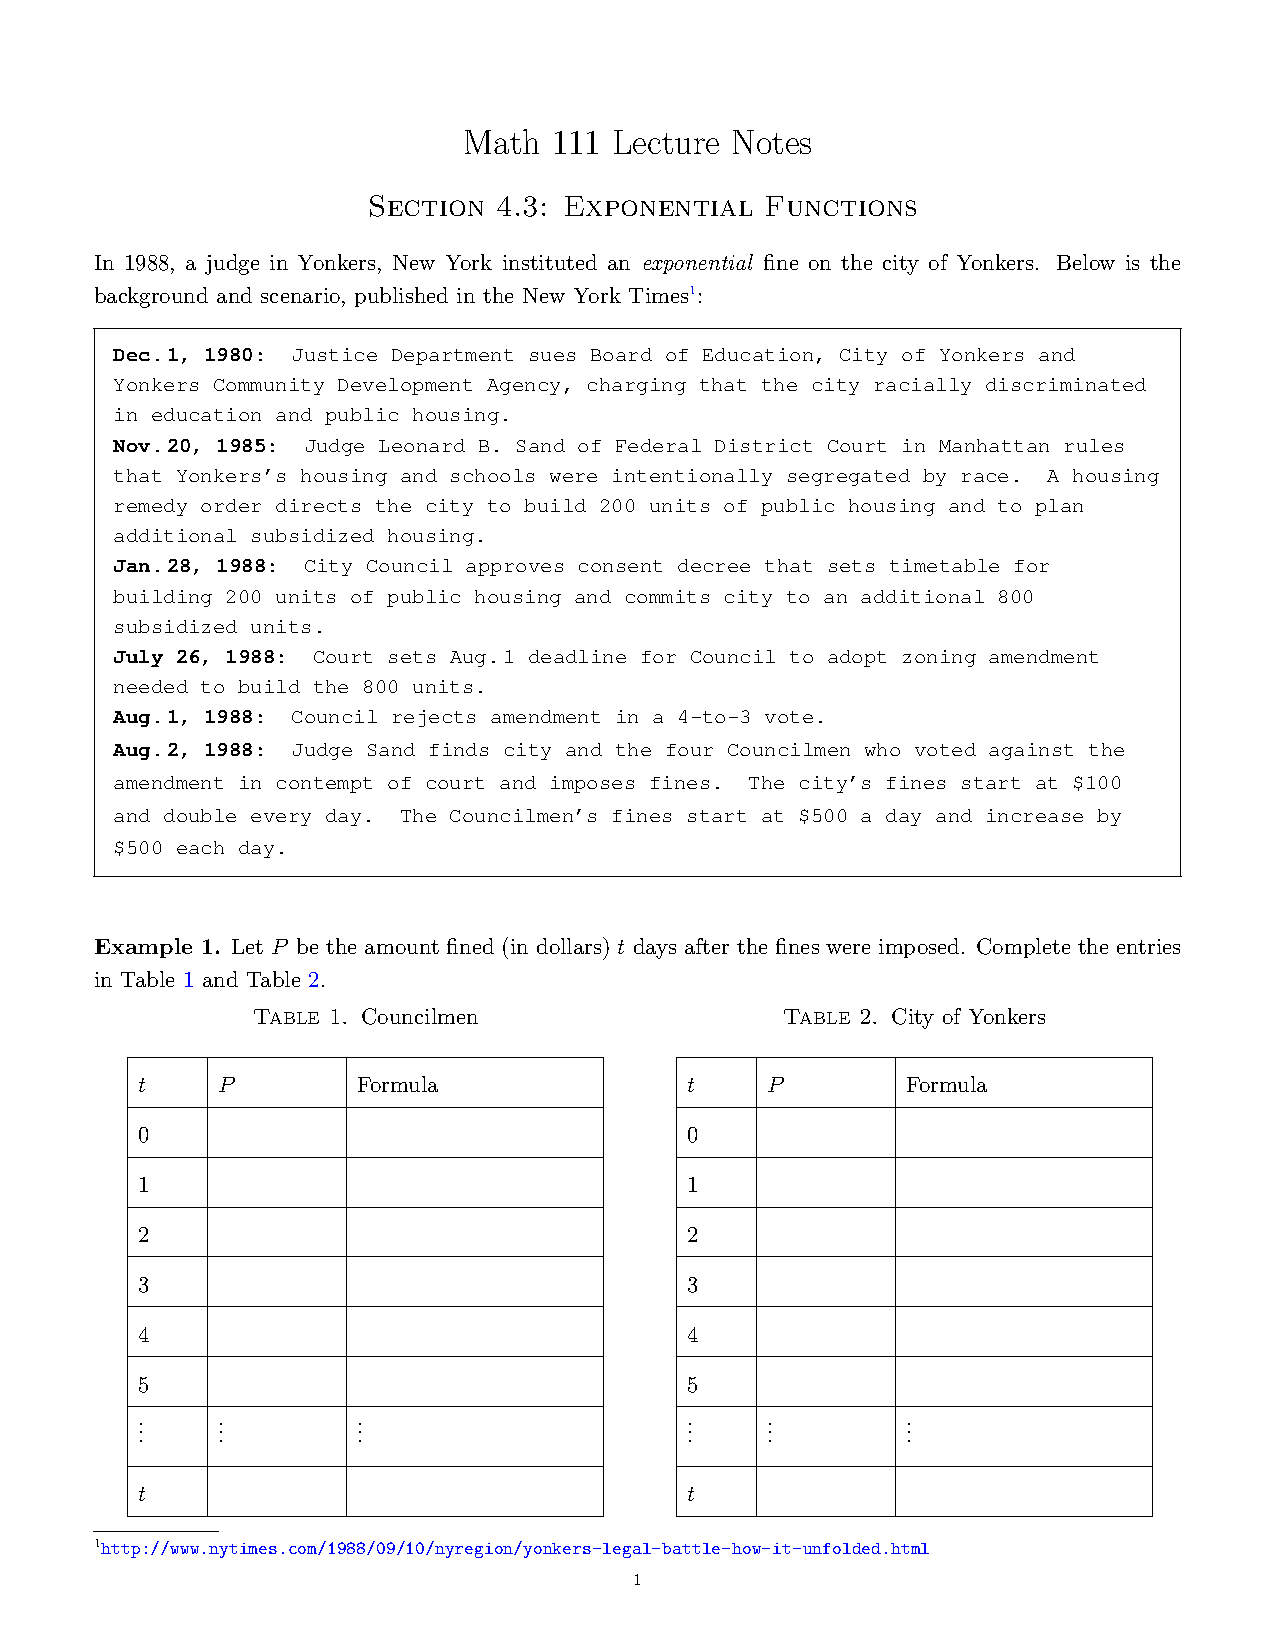
\includepdf[pages=-,pagecommand={\pagestyle{fancy}}]{./appendices/socialJusticeExample}

% arara: pdflatex: {files: [MathSACpr2014]}
% !arara: indent: {overwrite: yes}
\chapter{Class size report}\label{app:sec:classsize}
\emph{The report on the following pages was submitted to the DOIs}.

% http://tex.stackexchange.com/questions/117960/header-and-page-numbers-with-pdfpages
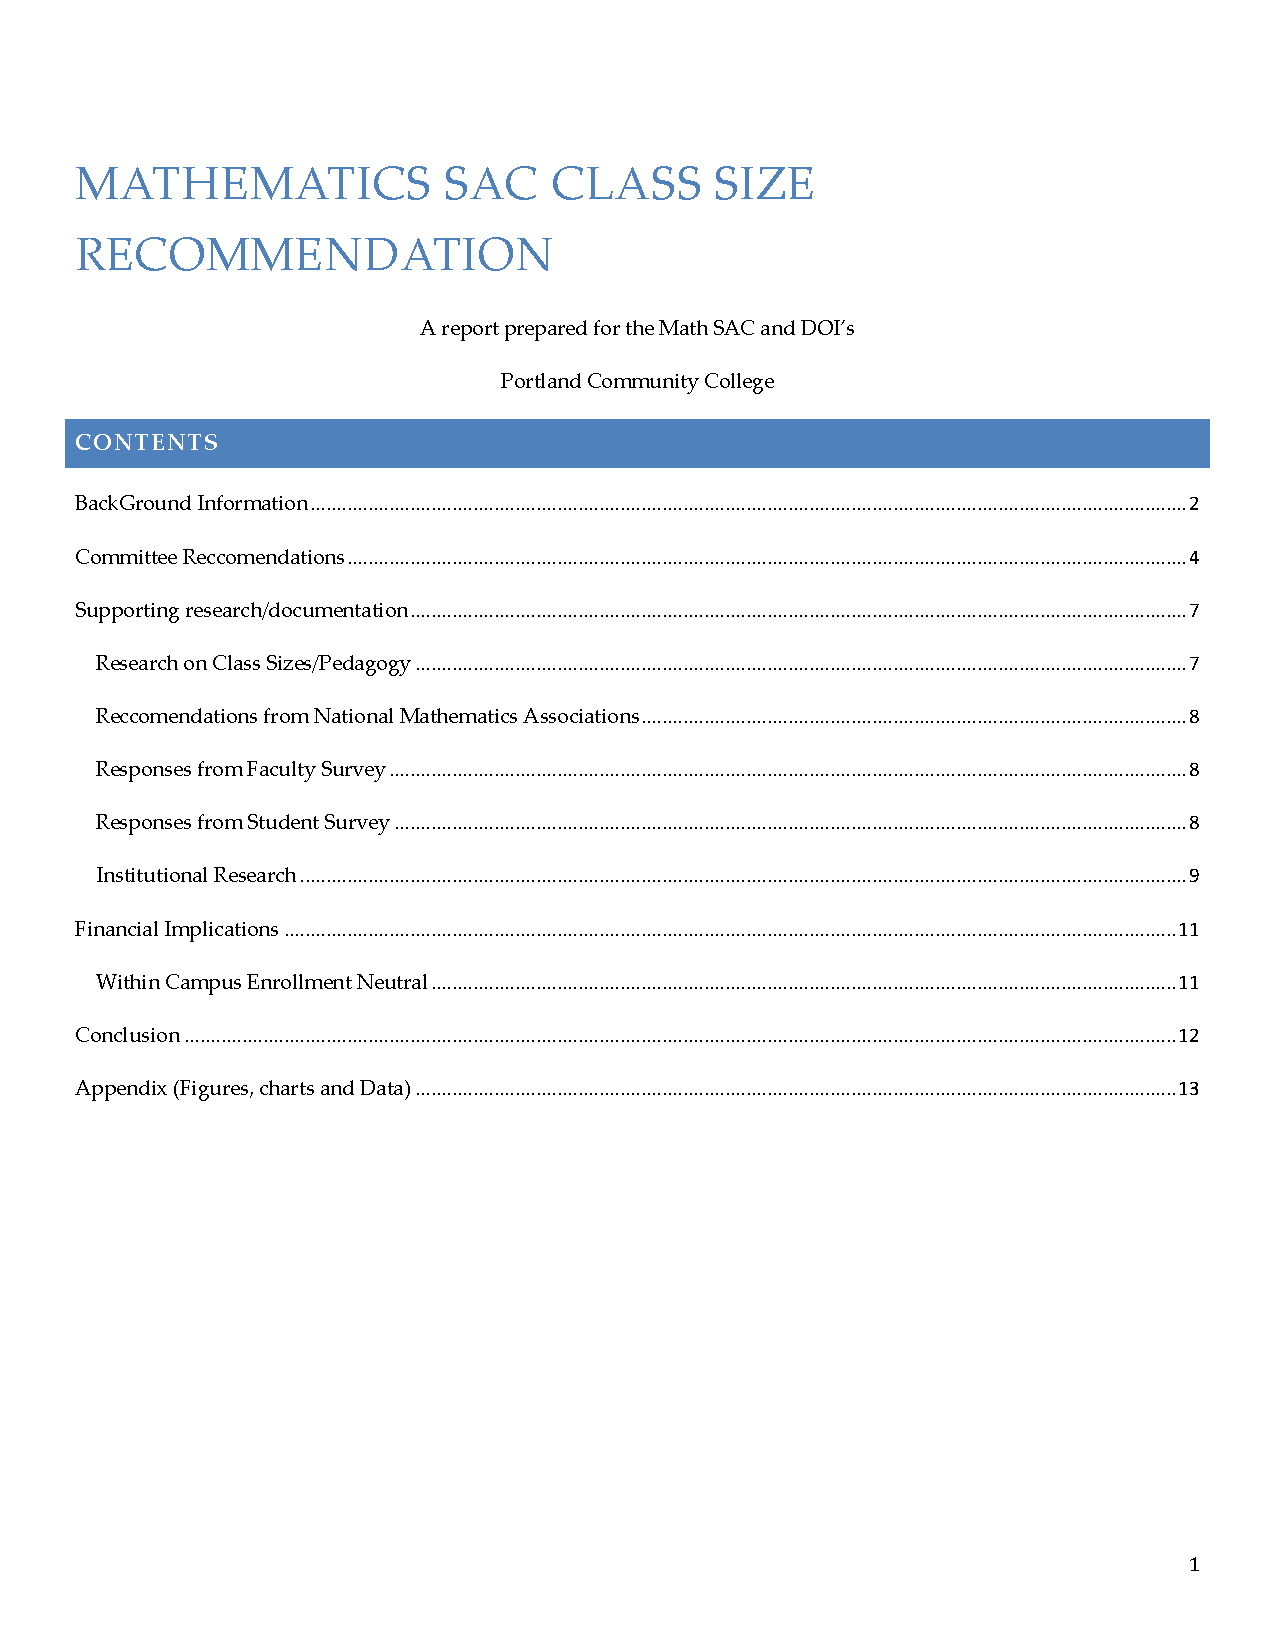
\includepdf[pages=-,pagecommand={\pagestyle{fancy}}]{appendices/classSizeRecommendations}

% arara: pdflatex: {files: [MathSACpr2014]}
% !arara: indent: {overwrite: yes}
\chapter{Demographic data}\label{app:sec:demographicdata}

\Crefrange{app:tab:demographic2008-2009}{app:tab:demographic2012-2013} show
demographic data for the academic years 2008 through 2013.

% the monster tables need bigger margins- don't worry, it
% is restored at the end
\newgeometry{left=0.5cm,right=0.5cm,
top=2cm,bottom=1.5cm,asymmetric=true,bindingoffset=0cm}
\begin{sidewaystable}
  \captionsetup{skip=0pt}
	\centering
	\caption{Demographic data for 2008--2009 (Pre-college level MTH and statistics)}
	% arara: pdflatex
\documentclass[varwidth]{standalone}
%\usepackage[landscape,textwidth=25cm]{geometry}
\usepackage{pgfplotstable}
\usepackage{booktabs}
\usepackage{multirow}

% caption: pass rates by demographic for 2008-2009
%           note that MTH 111 was split into MTH 111 A, B, C

% empty column type- very useful
\newcolumntype{H}{>{\setbox0=\hbox\bgroup}c<{\egroup}@{}}

\pgfplotstableset{percentstyle/.style={
    preproc/expr={##1*100},
    dec sep align,fixed,fixed zerofill,
postproc cell content/.append code={
            \ifx\\##1\\% check if ##1 is empty
            \else
            \ifnum1=\pgfplotstablepartno
                \pgfkeysalso{@cell content/.add={}{\,\%}}%
            \fi
            \fi
        },
    precision=0,
},
demographic/.style={},
}

% references:
%   http://tex.stackexchange.com/questions/65760/pgfplotstable-how-can-i-add-percent-signs-and-respect-dec-sep-align
%   http://tex.stackexchange.com/questions/16604/easiest-way-to-delete-a-column/16607#16607
%   http://tex.stackexchange.com/questions/89365/check-for-empty-macro-argument

\begin{document}

% http://tex.stackexchange.com/questions/128468/problems-with-pgfplotstableread-and-relative-paths
\IfStandalone{
	\newcommand{\fromRoot}[1]{../data/demographics/#1}
	}{
	\newcommand{\fromRoot}[1]{./data/demographics/#1}
}
\pgfplotstableread[col sep=comma]{\fromRoot{demographics2008-2009.csv}}\diversitydata

\noindent\resizebox{\textwidth}{!}{
\pgfplotstabletypeset[
every head row/.style={
        before row={%
        \toprule
        \multirow{2}{*}{2008--2009}
        & \multicolumn{7}{c}{MTH 20} 
        & \multicolumn{7}{c}{MTH 60} 
        & \multicolumn{7}{c}{MTH 65} 
        & \multicolumn{29}{c}{MTH 95} 
        & \multicolumn{10}{c}{MTH 243} 
        & \multicolumn{10}{c}{MTH 244} 
        \\},
        after row=\midrule},
every last row/.style={after row=\bottomrule},
every row no 3/.style={after row=\cmidrule{2-70}},
every row no 13/.style={after row=\cmidrule{2-70}},
demographic,
    columns/demographic/.style={string type,column name={},column type=l},
    % MTH 20 - ignore most of the columns
    columns/mth20p/.style={column type=H},
    columns/mth20np/.style={column type=H},
    columns/mth20tot/.style={column name=Total,column type=r},
    columns/mth20totper/.style={percentstyle,column name=\% Total},
    columns/mth20totpass/.style={percentstyle,column name=\% Pass},
    % MTH 60 - ignore most of the columns
    columns/mth60p/.style={column type=H},
    columns/mth60np/.style={column type=H},
    columns/mth60tot/.style={column name=Total,column type=r},
    columns/mth60totper/.style={percentstyle,column name=\% Total},
    columns/mth60totpass/.style={percentstyle,column name=\% Pass},
    % MTH 65 - ignore most of the columns
    columns/mth65p/.style={column type=H},
    columns/mth65np/.style={column type=H},
    columns/mth65tot/.style={column name=Total,column type=r},
    columns/mth65totper/.style={percentstyle,column name=\% Total},
    columns/mth65totpass/.style={percentstyle,column name=\% Pass},
    % MTH 95 - ignore most of the columns
    columns/mth95p/.style={column type=H},
    columns/mth95np/.style={column type=H},
    columns/mth95tot/.style={column name=Total,column type=r},
    columns/mth95totper/.style={percentstyle,column name=\% Total},
    columns/mth95totpass/.style={percentstyle,column name=\% Pass},
    % MTH 111A - ignore all of the columns
    columns/mth111Ap/.style={column type=H},
    columns/mth111Anp/.style={column type=H},
    columns/mth111Atot/.style={column type=H},
    columns/mth111Atotper/.style={column type=H},
    columns/mth111Atotpass/.style={column type=H},
    % MTH 111B - ignore all of the columns
    columns/mth111Bp/.style={column type=H},
    columns/mth111Bnp/.style={column type=H},
    columns/mth111Btot/.style={column type=H},
    columns/mth111Btotper/.style={column type=H},
    columns/mth111Btotpass/.style={column type=H},
    % MTH 111C - ignore all of the columns
    columns/mth111Cp/.style={column type=H},
    columns/mth111Cnp/.style={column type=H},
    columns/mth111Ctot/.style={column type=H},
    columns/mth111Ctotper/.style={column type=H},
    columns/mth111Ctotpass/.style={column type=H},
    % MTH 111BC - ignore most of the columns
    columns/mth111BCp/.style={column type=H},
    columns/mth111BCnp/.style={column type=H},
    columns/mth111BCtot/.style={column type=H},
    columns/mth111BCtotper/.style={column type=H},
    columns/mth111BCtotpass/.style={column type=H},
    % MTH 112 - ignore most of the columns
    columns/mth112p/.style={column type=H},
    columns/mth112np/.style={column type=H},
    columns/mth112tot/.style={column type=H},
    columns/mth112totper/.style={column type=H},
    columns/mth112totpass/.style={column type=H},
    % MTH 243 - ignore most of the columns
    columns/mth243p/.style={column type=H},
    columns/mth243np/.style={column type=H},
    columns/mth243tot/.style={column name=Total,column type=r},
    columns/mth243totper/.style={percentstyle,column name=\% Total},
    columns/mth243totpass/.style={percentstyle,column name=\% Pass},
    % MTH 244 - ignore most of the columns
    columns/mth244p/.style={column type=H},
    columns/mth244np/.style={column type=H},
    columns/mth244tot/.style={column name=Total,column type=r},
    columns/mth244totper/.style={percentstyle,column name=\% Total},
    columns/mth244totpass/.style={percentstyle,column name=\% Pass},
    % MTH 251 - ignore most of the columns
    columns/mth251p/.style={column type=H},
    columns/mth251np/.style={column type=H},
    columns/mth251tot/.style={column type=H},
    columns/mth251totper/.style={column type=H},
    columns/mth251totpass/.style={column type=H},
    % MTH 252 - ignore most of the columns
    columns/mth252p/.style={column type=H},
    columns/mth252np/.style={column type=H},
    columns/mth252tot/.style={column type=H},
    columns/mth252totper/.style={column type=H},
    columns/mth252totpass/.style={column type=H},
    % MTH 253 - ignore most of the columns
    columns/mth253p/.style={column type=H},
    columns/mth253np/.style={column type=H},
    columns/mth253tot/.style={column type=H},
    columns/mth253totper/.style={column type=H},
    columns/mth253totpass/.style={column type=H},
    % MTH 254 - ignore most of the columns
    columns/mth254p/.style={column type=H},
    columns/mth254np/.style={column type=H},
    columns/mth254tot/.style={column type=H},
    columns/mth254totper/.style={column type=H},
    columns/mth254totpass/.style={column type=H},
]{\diversitydata}
}

\end{document}

	\caption{Demographic data for 2008--2009 (College level MTH)}
	% arara: pdflatex
\documentclass[varwidth]{standalone}
%\usepackage[landscape,textwidth=25cm]{geometry}
\usepackage{pgfplotstable}
\usepackage{booktabs}
\usepackage{multirow}

% caption: pass rates by demographic for 2008-2009
%           note that MTH 111 was split into MTH 111 A, B, C

% empty column type- very useful
\newcolumntype{H}{>{\setbox0=\hbox\bgroup}c<{\egroup}@{}}

\pgfplotstableset{percentstyle/.style={
    preproc/expr={##1*100},
    dec sep align,fixed,fixed zerofill,
postproc cell content/.append code={
            \ifx\\##1\\% check if ##1 is empty
            \else
            \ifnum1=\pgfplotstablepartno
                \pgfkeysalso{@cell content/.add={}{\,\%}}%
            \fi
            \fi
        },
    precision=0,
}
}

% references:
%   http://tex.stackexchange.com/questions/65760/pgfplotstable-how-can-i-add-percent-signs-and-respect-dec-sep-align
%   http://tex.stackexchange.com/questions/16604/easiest-way-to-delete-a-column/16607#16607
%   http://tex.stackexchange.com/questions/89365/check-for-empty-macro-argument

\begin{document}

% http://tex.stackexchange.com/questions/128468/problems-with-pgfplotstableread-and-relative-paths
\IfStandalone{
	\newcommand{\fromRoot}[1]{../data/demographics/#1}
	}{
	\newcommand{\fromRoot}[1]{./data/demographics/#1}
}
\pgfplotstableread[col sep=comma]{\fromRoot{demographics2008-2009.csv}}\diversitydata

\noindent\resizebox{\textwidth}{!}{
\pgfplotstabletypeset[
every head row/.style={
        before row={%
        \toprule
        \multirow{2}{*}{2008--2009}
        & \multicolumn{30}{c}{MTH 111A} 
        & \multicolumn{15}{c}{MTH 111 B\&C} 
        & \multicolumn{11}{c}{MTH 112} 
        & \multicolumn{12}{c}{MTH 251} 
        & \multicolumn{7}{c}{MTH 252} 
        & \multicolumn{7}{c}{MTH 253} 
        & \multicolumn{7}{c}{MTH 254}\\},
        after row=\midrule},
every last row/.style={after row=\bottomrule},
every row no 3/.style={after row=\cmidrule{2-90}},
every row no 13/.style={after row=\cmidrule{2-90}},
    columns/demographic/.style={string type,column name={},column type=l},
    % MTH 20 - ignore most of the columns
    columns/mth20p/.style={column type=H},
    columns/mth20np/.style={column type=H},
    columns/mth20tot/.style={column type=H},
    columns/mth20totper/.style={column type=H},
    columns/mth20totpass/.style={column type=H},
    % MTH 60 - ignore most of the columns
    columns/mth60p/.style={column type=H},
    columns/mth60np/.style={column type=H},
    columns/mth60tot/.style={column type=H},
    columns/mth60totper/.style={column type=H},
    columns/mth60totpass/.style={column type=H},
    % MTH 65 - ignore most of the columns
    columns/mth65p/.style={column type=H},
    columns/mth65np/.style={column type=H},
    columns/mth65tot/.style={column type=H},
    columns/mth65totper/.style={column type=H},
    columns/mth65totpass/.style={column type=H},
    % MTH 95 - ignore most of the columns
    columns/mth95p/.style={column type=H},
    columns/mth95np/.style={column type=H},
    columns/mth95tot/.style={column type=H},
    columns/mth95totper/.style={column type=H},
    columns/mth95totpass/.style={column type=H},
    % MTH 111A - ignore all of the columns
    columns/mth111Ap/.style={column type=H},
    columns/mth111Anp/.style={column type=H},
    columns/mth111Atot/.style={column name=Total,column type=r},
    columns/mth111Atotper/.style={percentstyle,column name=\% Total},
    columns/mth111Atotpass/.style={percentstyle,column name=\% Pass},
    % MTH 111B - ignore all of the columns
    columns/mth111Bp/.style={column type=H},
    columns/mth111Bnp/.style={column type=H},
    columns/mth111Btot/.style={column type=H},
    columns/mth111Btotper/.style={column type=H},
    columns/mth111Btotpass/.style={column type=H},
    % MTH 111C - ignore all of the columns
    columns/mth111Cp/.style={column type=H},
    columns/mth111Cnp/.style={column type=H},
    columns/mth111Ctot/.style={column type=H},
    columns/mth111Ctotper/.style={column type=H},
    columns/mth111Ctotpass/.style={column type=H},
    % MTH 111BC - ignore most of the columns
    columns/mth111BCp/.style={column type=H},
    columns/mth111BCnp/.style={column type=H},
    columns/mth111BCtot/.style={column name=Total,column type=r},
    columns/mth111BCtotper/.style={percentstyle,column name=\% Total},
    columns/mth111BCtotpass/.style={percentstyle,column name=\% Pass},
    % MTH 112 - ignore most of the columns
    columns/mth112p/.style={column type=H},
    columns/mth112np/.style={column type=H},
    columns/mth112tot/.style={column name=Total,column type=r},
    columns/mth112totper/.style={percentstyle,column name=\% Total},
    columns/mth112totpass/.style={percentstyle,column name=\% Pass},
    % MTH 243 - ignore most of the columns
    columns/mth243p/.style={column type=H},
    columns/mth243np/.style={column type=H},
    columns/mth243tot/.style={column type=H},
    columns/mth243totper/.style={column type=H},
    columns/mth243totpass/.style={column type=H},
    % MTH 244 - ignore most of the columns
    columns/mth244p/.style={column type=H},
    columns/mth244np/.style={column type=H},
    columns/mth244tot/.style={column type=H},
    columns/mth244totper/.style={column type=H},
    columns/mth244totpass/.style={column type=H},
    % MTH 251 - ignore most of the columns
    columns/mth251p/.style={column type=H},
    columns/mth251np/.style={column type=H},
    columns/mth251tot/.style={column name=Total,column type=r},
    columns/mth251totper/.style={percentstyle,column name=\% Total},
    columns/mth251totpass/.style={percentstyle,column name=\% Pass},
    % MTH 252 - ignore most of the columns
    columns/mth252p/.style={column type=H},
    columns/mth252np/.style={column type=H},
    columns/mth252tot/.style={column name=Total,column type=r},
    columns/mth252totper/.style={percentstyle,column name=\% Total},
    columns/mth252totpass/.style={percentstyle,column name=\% Pass},
    % MTH 253 - ignore most of the columns
    columns/mth253p/.style={column type=H},
    columns/mth253np/.style={column type=H},
    columns/mth253tot/.style={column name=Total,column type=r},
    columns/mth253totper/.style={percentstyle,column name=\% Total},
    columns/mth253totpass/.style={percentstyle,column name=\% Pass},
    % MTH 254 - ignore most of the columns
    columns/mth254p/.style={column type=H},
    columns/mth254np/.style={column type=H},
    columns/mth254tot/.style={column name=Total,column type=r},
    columns/mth254totper/.style={percentstyle,column name=\% Total},
    columns/mth254totpass/.style={percentstyle,column name=\% Pass},
]{\diversitydata}
}

\end{document}

\end{sidewaystable}
\begin{sidewaystable}
  \captionsetup{skip=0pt}
	\centering
	\caption{Demographic data for 2009--2010 (Pre-college level MTH and statistics)}
	% arara: pdflatex
\documentclass[varwidth]{standalone}
%\usepackage[landscape,textwidth=25cm]{geometry}
\usepackage{pgfplotstable}
\usepackage{booktabs}
\usepackage{multirow}

% caption: pass rates by demographic for 2009-2010
%           note that MTH 111 was split into MTH 111 A, B, C
%           and that there was 0 enrollment in MTH 111A which is
%           why it is not displayed.

% empty column type- very useful
\newcolumntype{H}{>{\setbox0=\hbox\bgroup}c<{\egroup}@{}}

\pgfplotstableset{percentstyle/.style={
    preproc/expr={##1*100},
    dec sep align,fixed,fixed zerofill,
postproc cell content/.append code={
            \ifx\\##1\\% check if ##1 is empty
            \else
            \ifnum1=\pgfplotstablepartno
                \pgfkeysalso{@cell content/.add={}{\,\%}}%
            \fi
            \fi
        },
    precision=0,
}
}

% references:
%   http://tex.stackexchange.com/questions/65760/pgfplotstable-how-can-i-add-percent-signs-and-respect-dec-sep-align
%   http://tex.stackexchange.com/questions/16604/easiest-way-to-delete-a-column/16607#16607
%   http://tex.stackexchange.com/questions/89365/check-for-empty-macro-argument

\begin{document}

% http://tex.stackexchange.com/questions/128468/problems-with-pgfplotstableread-and-relative-paths
\IfStandalone{
	\newcommand{\fromRoot}[1]{../data/demographics/#1}
	}{
	\newcommand{\fromRoot}[1]{./data/demographics/#1}
}

\pgfplotstableread[col sep=comma]{\fromRoot{demographics2009-2010.csv}}\diversitydata

%Note that MTH 111A had $0$ enrollment for 2009--2010, so its data is not displayed.

\noindent\resizebox{\textwidth}{!}{
\pgfplotstabletypeset[
every head row/.style={
        before row={%
        \toprule
        \multirow{2}{*}{2009--2010}
        & \multicolumn{7}{c}{MTH 20} 
        & \multicolumn{7}{c}{MTH 60} 
        & \multicolumn{7}{c}{MTH 65} 
        & \multicolumn{29}{c}{MTH 95} 
        & \multicolumn{10}{c}{MTH 243} 
        & \multicolumn{10}{c}{MTH 244} 
        \\},
        after row=\midrule},
every last row/.style={after row=\bottomrule},
every row no 3/.style={after row=\cmidrule{2-80}},
every row no 13/.style={after row=\cmidrule{2-80}},
    columns/demographic/.style={string type,column name={},column type=l},
    % MTH 20 - ignore most of the columns
    columns/mth20p/.style={column type=H},
    columns/mth20np/.style={column type=H},
    columns/mth20tot/.style={column name=Total,column type=r},
    columns/mth20totper/.style={percentstyle,column name=\% Total},
    columns/mth20totpass/.style={percentstyle,column name=\% Pass},
    % MTH 60 - ignore most of the columns
    columns/mth60p/.style={column type=H},
    columns/mth60np/.style={column type=H},
    columns/mth60tot/.style={column name=Total,column type=r},
    columns/mth60totper/.style={percentstyle,column name=\% Total},
    columns/mth60totpass/.style={percentstyle,column name=\% Pass},
    % MTH 65 - ignore most of the columns
    columns/mth65p/.style={column type=H},
    columns/mth65np/.style={column type=H},
    columns/mth65tot/.style={column name=Total,column type=r},
    columns/mth65totper/.style={percentstyle,column name=\% Total},
    columns/mth65totpass/.style={percentstyle,column name=\% Pass},
    % MTH 95 - ignore most of the columns
    columns/mth95p/.style={column type=H},
    columns/mth95np/.style={column type=H},
    columns/mth95tot/.style={column name=Total,column type=r},
    columns/mth95totper/.style={percentstyle,column name=\% Total},
    columns/mth95totpass/.style={percentstyle,column name=\% Pass},
    % MTH 111A - ignore all of the columns
    columns/mth111Ap/.style={column type=H},
    columns/mth111Anp/.style={column type=H},
    columns/mth111Atot/.style={column type=H},
    columns/mth111Atotper/.style={column type=H},
    columns/mth111Atotpass/.style={column type=H},
    % MTH 111B - ignore all of the columns
    columns/mth111Bp/.style={column type=H},
    columns/mth111Bnp/.style={column type=H},
    columns/mth111Btot/.style={column type=H},
    columns/mth111Btotper/.style={column type=H},
    columns/mth111Btotpass/.style={column type=H},
    % MTH 111C - ignore all of the columns
    columns/mth111Cp/.style={column type=H},
    columns/mth111Cnp/.style={column type=H},
    columns/mth111Ctot/.style={column type=H},
    columns/mth111Ctotper/.style={column type=H},
    columns/mth111Ctotpass/.style={column type=H},
    % MTH 111BC - ignore most of the columns
    columns/mth111BCp/.style={column type=H},
    columns/mth111BCnp/.style={column type=H},
    columns/mth111BCtot/.style={column type=H},
    columns/mth111BCtotper/.style={column type=H},
    columns/mth111BCtotpass/.style={column type=H},
    % MTH 112 - ignore most of the columns
    columns/mth112p/.style={column type=H},
    columns/mth112np/.style={column type=H},
    columns/mth112tot/.style={column type=H},
    columns/mth112totper/.style={column type=H},
    columns/mth112totpass/.style={column type=H},
    % MTH 243 - ignore most of the columns
    columns/mth243p/.style={column type=H},
    columns/mth243np/.style={column type=H},
    columns/mth243tot/.style={column name=Total,column type=r},
    columns/mth243totper/.style={percentstyle,column name=\% Total},
    columns/mth243totpass/.style={percentstyle,column name=\% Pass},
    % MTH 244 - ignore most of the columns
    columns/mth244p/.style={column type=H},
    columns/mth244np/.style={column type=H},
    columns/mth244tot/.style={column name=Total,column type=r},
    columns/mth244totper/.style={percentstyle,column name=\% Total},
    columns/mth244totpass/.style={percentstyle,column name=\% Pass},
    % MTH 251 - ignore most of the columns
    columns/mth251p/.style={column type=H},
    columns/mth251np/.style={column type=H},
    columns/mth251tot/.style={column type=H},
    columns/mth251totper/.style={column type=H},
    columns/mth251totpass/.style={column type=H},
    % MTH 252 - ignore most of the columns
    columns/mth252p/.style={column type=H},
    columns/mth252np/.style={column type=H},
    columns/mth252tot/.style={column type=H},
    columns/mth252totper/.style={column type=H},
    columns/mth252totpass/.style={column type=H},
    % MTH 253 - ignore most of the columns
    columns/mth253p/.style={column type=H},
    columns/mth253np/.style={column type=H},
    columns/mth253tot/.style={column type=H},
    columns/mth253totper/.style={column type=H},
    columns/mth253totpass/.style={column type=H},
    % MTH 254 - ignore most of the columns
    columns/mth254p/.style={column type=H},
    columns/mth254np/.style={column type=H},
    columns/mth254tot/.style={column type=H},
    columns/mth254totper/.style={column type=H},
    columns/mth254totpass/.style={column type=H},
]{\diversitydata}
}

\end{document}

	\caption{Demographic data for 2009--2010 (College level MTH). Note that MTH 111A had $0$ enrollment for 2009--2010, so its data is not displayed. }
	% arara: pdflatex
\documentclass[varwidth]{standalone}
%\usepackage[landscape,textwidth=25cm]{geometry}
\usepackage{pgfplotstable}
\usepackage{booktabs}
\usepackage{multirow}

% caption: pass rates by demographic for 2009-2010
%           note that MTH 111 was split into MTH 111 A, B, C
%           and that there was 0 enrollment in MTH 111A which is
%           why it is not displayed.

% empty column type- very useful
\newcolumntype{H}{>{\setbox0=\hbox\bgroup}c<{\egroup}@{}}

\pgfplotstableset{percentstyle/.style={
    preproc/expr={##1*100},
    dec sep align,fixed,fixed zerofill,
postproc cell content/.append code={
            \ifx\\##1\\% check if ##1 is empty
            \else
            \ifnum1=\pgfplotstablepartno
                \pgfkeysalso{@cell content/.add={}{\,\%}}%
            \fi
            \fi
        },
    precision=0,
}
}

% references:
%   http://tex.stackexchange.com/questions/65760/pgfplotstable-how-can-i-add-percent-signs-and-respect-dec-sep-align
%   http://tex.stackexchange.com/questions/16604/easiest-way-to-delete-a-column/16607#16607
%   http://tex.stackexchange.com/questions/89365/check-for-empty-macro-argument

\begin{document}

% http://tex.stackexchange.com/questions/128468/problems-with-pgfplotstableread-and-relative-paths
\IfStandalone{
	\newcommand{\fromRoot}[1]{../data/demographics/#1}
	}{
	\newcommand{\fromRoot}[1]{./data/demographics/#1}
}

\pgfplotstableread[col sep=comma]{\fromRoot{demographics2009-2010.csv}}\diversitydata

%Note that MTH 111A had $0$ enrollment for 2009--2010, so its data is not displayed.

\noindent\resizebox{\textwidth}{!}{
\pgfplotstabletypeset[
every head row/.style={
        before row={%
        \toprule
        \multirow{2}{*}{2009--2010}
        & \multicolumn{44}{c}{MTH 111 B\&C}
        & \multicolumn{5}{c}{MTH 112} 
        & \multicolumn{17}{c}{MTH 251} 
        & \multicolumn{7}{c}{MTH 252} 
        & \multicolumn{7}{c}{MTH 253} 
        & \multicolumn{7}{c}{MTH 254}\\},
        after row=\midrule},
every last row/.style={after row=\bottomrule},
every row no 3/.style={after row=\cmidrule{2-80}},
every row no 13/.style={after row=\cmidrule{2-80}},
    columns/demographic/.style={string type,column name={},column type=l},
    % MTH 20 - ignore most of the columns
    columns/mth20p/.style={column type=H},
    columns/mth20np/.style={column type=H},
    columns/mth20tot/.style={column type=H},
    columns/mth20totper/.style={column type=H},
    columns/mth20totpass/.style={column type=H},
    % MTH 60 - ignore most of the columns
    columns/mth60p/.style={column type=H},
    columns/mth60np/.style={column type=H},
    columns/mth60tot/.style={column type=H},
    columns/mth60totper/.style={column type=H},
    columns/mth60totpass/.style={column type=H},
    % MTH 65 - ignore most of the columns
    columns/mth65p/.style={column type=H},
    columns/mth65np/.style={column type=H},
    columns/mth65tot/.style={column type=H},
    columns/mth65totper/.style={column type=H},
    columns/mth65totpass/.style={column type=H},
    % MTH 95 - ignore most of the columns
    columns/mth95p/.style={column type=H},
    columns/mth95np/.style={column type=H},
    columns/mth95tot/.style={column type=H},
    columns/mth95totper/.style={column type=H},
    columns/mth95totpass/.style={column type=H},
    % MTH 111A - ignore all of the columns
    columns/mth111Ap/.style={column type=H},
    columns/mth111Anp/.style={column type=H},
    columns/mth111Atot/.style={column type=H},
    columns/mth111Atotper/.style={column type=H},
    columns/mth111Atotpass/.style={column type=H},
    % MTH 111B - ignore all of the columns
    columns/mth111Bp/.style={column type=H},
    columns/mth111Bnp/.style={column type=H},
    columns/mth111Btot/.style={column type=H},
    columns/mth111Btotper/.style={column type=H},
    columns/mth111Btotpass/.style={column type=H},
    % MTH 111C - ignore all of the columns
    columns/mth111Cp/.style={column type=H},
    columns/mth111Cnp/.style={column type=H},
    columns/mth111Ctot/.style={column type=H},
    columns/mth111Ctotper/.style={column type=H},
    columns/mth111Ctotpass/.style={column type=H},
    % MTH 111BC - ignore most of the columns
    columns/mth111BCp/.style={column type=H},
    columns/mth111BCnp/.style={column type=H},
    columns/mth111BCtot/.style={column name=Total,column type=r},
    columns/mth111BCtotper/.style={percentstyle,column name=\% Total},
    columns/mth111BCtotpass/.style={percentstyle,column name=\% Pass},
    % MTH 112 - ignore most of the columns
    columns/mth112p/.style={column type=H},
    columns/mth112np/.style={column type=H},
    columns/mth112tot/.style={column name=Total,column type=r},
    columns/mth112totper/.style={percentstyle,column name=\% Total},
    columns/mth112totpass/.style={percentstyle,column name=\% Pass},
    % MTH 243 - ignore most of the columns
    columns/mth243p/.style={column type=H},
    columns/mth243np/.style={column type=H},
    columns/mth243tot/.style={column type=H},
    columns/mth243totper/.style={column type=H},
    columns/mth243totpass/.style={column type=H},
    % MTH 244 - ignore most of the columns
    columns/mth244p/.style={column type=H},
    columns/mth244np/.style={column type=H},
    columns/mth244tot/.style={column type=H},
    columns/mth244totper/.style={column type=H},
    columns/mth244totpass/.style={column type=H},
    % MTH 251 - ignore most of the columns
    columns/mth251p/.style={column type=H},
    columns/mth251np/.style={column type=H},
    columns/mth251tot/.style={column name=Total,column type=r},
    columns/mth251totper/.style={percentstyle,column name=\% Total},
    columns/mth251totpass/.style={percentstyle,column name=\% Pass},
    % MTH 252 - ignore most of the columns
    columns/mth252p/.style={column type=H},
    columns/mth252np/.style={column type=H},
    columns/mth252tot/.style={column name=Total,column type=r},
    columns/mth252totper/.style={percentstyle,column name=\% Total},
    columns/mth252totpass/.style={percentstyle,column name=\% Pass},
    % MTH 253 - ignore most of the columns
    columns/mth253p/.style={column type=H},
    columns/mth253np/.style={column type=H},
    columns/mth253tot/.style={column name=Total,column type=r},
    columns/mth253totper/.style={percentstyle,column name=\% Total},
    columns/mth253totpass/.style={percentstyle,column name=\% Pass},
    % MTH 254 - ignore most of the columns
    columns/mth254p/.style={column type=H},
    columns/mth254np/.style={column type=H},
    columns/mth254tot/.style={column name=Total,column type=r},
    columns/mth254totper/.style={percentstyle,column name=\% Total},
    columns/mth254totpass/.style={percentstyle,column name=\% Pass},
]{\diversitydata}
}

\end{document}

\end{sidewaystable}
\begin{sidewaystable}
  \captionsetup{skip=0pt}
	\centering
	\caption{Demographic data for 2010--2011 (Pre-college level MTH and statistics)}
	% arara: pdflatex
\documentclass[varwidth]{standalone}
%\usepackage[landscape,textwidth=25cm]{geometry}
\usepackage{pgfplotstable}
\usepackage{booktabs}
\usepackage{multirow}

% caption: pass rates by demographic for 2010-2011
%           note that MTH 111 was split into MTH 111 A, B, C
%           and that there was 0 enrollment in MTH 111A which is
%           why it is not displayed.

% empty column type- very useful
\newcolumntype{H}{>{\setbox0=\hbox\bgroup}c<{\egroup}@{}}

\pgfplotstableset{percentstyle/.style={
    preproc/expr={##1*100},
    dec sep align,fixed,fixed zerofill,
postproc cell content/.append code={
            \ifx\\##1\\% check if ##1 is empty
            \else
            \ifnum1=\pgfplotstablepartno
                \pgfkeysalso{@cell content/.add={}{\,\%}}%
            \fi
            \fi
        },
    precision=0,
}
}

% references:
%   http://tex.stackexchange.com/questions/65760/pgfplotstable-how-can-i-add-percent-signs-and-respect-dec-sep-align
%   http://tex.stackexchange.com/questions/16604/easiest-way-to-delete-a-column/16607#16607
%   http://tex.stackexchange.com/questions/89365/check-for-empty-macro-argument

\begin{document}

% http://tex.stackexchange.com/questions/128468/problems-with-pgfplotstableread-and-relative-paths
\IfStandalone{
	\newcommand{\fromRoot}[1]{../data/demographics/#1}
	}{
	\newcommand{\fromRoot}[1]{./data/demographics/#1}
}
\pgfplotstableread[col sep=comma]{\fromRoot{demographics2010-2011.csv}}\diversitydata

%Note that MTH 111A had $0$ enrollment for 2010--2011, so its data is not displayed.

\noindent\resizebox{\textwidth}{!}{
\pgfplotstabletypeset[
every head row/.style={
        before row={%
        \toprule
        \multirow{2}{*}{2010--2011}
        & \multicolumn{7}{c}{MTH 20} 
        & \multicolumn{7}{c}{MTH 60} 
        & \multicolumn{7}{c}{MTH 65} 
        & \multicolumn{29}{c}{MTH 95} 
        & \multicolumn{10}{c}{MTH 243} 
        & \multicolumn{10}{c}{MTH 244} 
        \\},
        after row=\midrule},
every last row/.style={after row=\bottomrule},
every row no 3/.style={after row=\cmidrule{2-80}},
every row no 13/.style={after row=\cmidrule{2-80}},
    columns/demographic/.style={string type,column name={},column type=l},
    % MTH 20 - ignore most of the columns
    columns/mth20p/.style={column type=H},
    columns/mth20np/.style={column type=H},
    columns/mth20tot/.style={column name=Total,column type=r},
    columns/mth20totper/.style={percentstyle,column name=\% Total},
    columns/mth20totpass/.style={percentstyle,column name=\% Pass},
    % MTH 60 - ignore most of the columns
    columns/mth60p/.style={column type=H},
    columns/mth60np/.style={column type=H},
    columns/mth60tot/.style={column name=Total,column type=r},
    columns/mth60totper/.style={percentstyle,column name=\% Total},
    columns/mth60totpass/.style={percentstyle,column name=\% Pass},
    % MTH 65 - ignore most of the columns
    columns/mth65p/.style={column type=H},
    columns/mth65np/.style={column type=H},
    columns/mth65tot/.style={column name=Total,column type=r},
    columns/mth65totper/.style={percentstyle,column name=\% Total},
    columns/mth65totpass/.style={percentstyle,column name=\% Pass},
    % MTH 95 - ignore most of the columns
    columns/mth95p/.style={column type=H},
    columns/mth95np/.style={column type=H},
    columns/mth95tot/.style={column name=Total,column type=r},
    columns/mth95totper/.style={percentstyle,column name=\% Total},
    columns/mth95totpass/.style={percentstyle,column name=\% Pass},
    % MTH 111A - ignore all of the columns
    columns/mth111Ap/.style={column type=H},
    columns/mth111Anp/.style={column type=H},
    columns/mth111Atot/.style={column type=H},
    columns/mth111Atotper/.style={column type=H},
    columns/mth111Atotpass/.style={column type=H},
    % MTH 111B - ignore all of the columns
    columns/mth111Bp/.style={column type=H},
    columns/mth111Bnp/.style={column type=H},
    columns/mth111Btot/.style={column type=H},
    columns/mth111Btotper/.style={column type=H},
    columns/mth111Btotpass/.style={column type=H},
    % MTH 111C - ignore all of the columns
    columns/mth111Cp/.style={column type=H},
    columns/mth111Cnp/.style={column type=H},
    columns/mth111Ctot/.style={column type=H},
    columns/mth111Ctotper/.style={column type=H},
    columns/mth111Ctotpass/.style={column type=H},
    % MTH 111BC - ignore most of the columns
    columns/mth111BCp/.style={column type=H},
    columns/mth111BCnp/.style={column type=H},
    columns/mth111BCtot/.style={column type=H},
    columns/mth111BCtotper/.style={column type=H},
    columns/mth111BCtotpass/.style={column type=H},
    % MTH 112 - ignore most of the columns
    columns/mth112p/.style={column type=H},
    columns/mth112np/.style={column type=H},
    columns/mth112tot/.style={column type=H},
    columns/mth112totper/.style={column type=H},
    columns/mth112totpass/.style={column type=H},
    % MTH 243 - ignore most of the columns
    columns/mth243p/.style={column type=H},
    columns/mth243np/.style={column type=H},
    columns/mth243tot/.style={column name=Total,column type=r},
    columns/mth243totper/.style={percentstyle,column name=\% Total},
    columns/mth243totpass/.style={percentstyle,column name=\% Pass},
    % MTH 244 - ignore most of the columns
    columns/mth244p/.style={column type=H},
    columns/mth244np/.style={column type=H},
    columns/mth244tot/.style={column name=Total,column type=r},
    columns/mth244totper/.style={percentstyle,column name=\% Total},
    columns/mth244totpass/.style={percentstyle,column name=\% Pass},
    % MTH 251 - ignore most of the columns
    columns/mth251p/.style={column type=H},
    columns/mth251np/.style={column type=H},
    columns/mth251tot/.style={column type=H},
    columns/mth251totper/.style={column type=H},
    columns/mth251totpass/.style={column type=H},
    % MTH 252 - ignore most of the columns
    columns/mth252p/.style={column type=H},
    columns/mth252np/.style={column type=H},
    columns/mth252tot/.style={column type=H},
    columns/mth252totper/.style={column type=H},
    columns/mth252totpass/.style={column type=H},
    % MTH 253 - ignore most of the columns
    columns/mth253p/.style={column type=H},
    columns/mth253np/.style={column type=H},
    columns/mth253tot/.style={column type=H},
    columns/mth253totper/.style={column type=H},
    columns/mth253totpass/.style={column type=H},
    % MTH 254 - ignore most of the columns
    columns/mth254p/.style={column type=H},
    columns/mth254np/.style={column type=H},
    columns/mth254tot/.style={column type=H},
    columns/mth254totper/.style={column type=H},
    columns/mth254totpass/.style={column type=H},
]{\diversitydata}
}

\end{document}

	\caption{Demographic data for 2010--2011 (College level MTH). Note that MTH 111A had $0$ enrollment for 2010--2011, so its data is not displayed. }
	% arara: pdflatex
\documentclass[varwidth]{standalone}
%\usepackage[landscape,textwidth=25cm]{geometry}
\usepackage{pgfplotstable}
\usepackage{booktabs}
\usepackage{multirow}

% caption: pass rates by demographic for 2010-2011
%           note that MTH 111 was split into MTH 111 A, B, C
%           and that there was 0 enrollment in MTH 111A which is
%           why it is not displayed.

% empty column type- very useful
\newcolumntype{H}{>{\setbox0=\hbox\bgroup}c<{\egroup}@{}}

\pgfplotstableset{percentstyle/.style={
    preproc/expr={##1*100},
    dec sep align,fixed,fixed zerofill,
postproc cell content/.append code={
            \ifx\\##1\\% check if ##1 is empty
            \else
            \ifnum1=\pgfplotstablepartno
                \pgfkeysalso{@cell content/.add={}{\,\%}}%
            \fi
            \fi
        },
    precision=0,
}
}

% references:
%   http://tex.stackexchange.com/questions/65760/pgfplotstable-how-can-i-add-percent-signs-and-respect-dec-sep-align
%   http://tex.stackexchange.com/questions/16604/easiest-way-to-delete-a-column/16607#16607
%   http://tex.stackexchange.com/questions/89365/check-for-empty-macro-argument

\begin{document}

% http://tex.stackexchange.com/questions/128468/problems-with-pgfplotstableread-and-relative-paths
\IfStandalone{
	\newcommand{\fromRoot}[1]{../data/demographics/#1}
	}{
	\newcommand{\fromRoot}[1]{./data/demographics/#1}
}
\pgfplotstableread[col sep=comma]{\fromRoot{demographics2010-2011.csv}}\diversitydata

%Note that MTH 111A had $0$ enrollment for 2010--2011, so its data is not displayed.

\noindent\resizebox{\textwidth}{!}{
\pgfplotstabletypeset[
every head row/.style={
        before row={%
        \toprule
        \multirow{2}{*}{2010--2011}
        & \multicolumn{44}{c}{MTH 111 B\&C}
        & \multicolumn{5}{c}{MTH 112} 
        & \multicolumn{17}{c}{MTH 251} 
        & \multicolumn{7}{c}{MTH 252} 
        & \multicolumn{7}{c}{MTH 253} 
        & \multicolumn{7}{c}{MTH 254}\\},
        after row=\midrule},
every last row/.style={after row=\bottomrule},
every row no 3/.style={after row=\cmidrule{2-88}},
every row no 13/.style={after row=\cmidrule{2-88}},
    columns/demographic/.style={string type,column name={},column type=l},
    % MTH 20 - ignore most of the columns
    columns/mth20p/.style={column type=H},
    columns/mth20np/.style={column type=H},
    columns/mth20tot/.style={column type=H},
    columns/mth20totper/.style={column type=H},
    columns/mth20totpass/.style={column type=H},
    % MTH 60 - ignore most of the columns
    columns/mth60p/.style={column type=H},
    columns/mth60np/.style={column type=H},
    columns/mth60tot/.style={column type=H},
    columns/mth60totper/.style={column type=H},
    columns/mth60totpass/.style={column type=H},
    % MTH 65 - ignore most of the columns
    columns/mth65p/.style={column type=H},
    columns/mth65np/.style={column type=H},
    columns/mth65tot/.style={column type=H},
    columns/mth65totper/.style={column type=H},
    columns/mth65totpass/.style={column type=H},
    % MTH 95 - ignore most of the columns
    columns/mth95p/.style={column type=H},
    columns/mth95np/.style={column type=H},
    columns/mth95tot/.style={column type=H},
    columns/mth95totper/.style={column type=H},
    columns/mth95totpass/.style={column type=H},
    % MTH 111A - ignore all of the columns
    columns/mth111Ap/.style={column type=H},
    columns/mth111Anp/.style={column type=H},
    columns/mth111Atot/.style={column type=H},
    columns/mth111Atotper/.style={column type=H},
    columns/mth111Atotpass/.style={column type=H},
    % MTH 111B - ignore all of the columns
    columns/mth111Bp/.style={column type=H},
    columns/mth111Bnp/.style={column type=H},
    columns/mth111Btot/.style={column type=H},
    columns/mth111Btotper/.style={column type=H},
    columns/mth111Btotpass/.style={column type=H},
    % MTH 111C - ignore all of the columns
    columns/mth111Cp/.style={column type=H},
    columns/mth111Cnp/.style={column type=H},
    columns/mth111Ctot/.style={column type=H},
    columns/mth111Ctotper/.style={column type=H},
    columns/mth111Ctotpass/.style={column type=H},
    % MTH 111BC - ignore most of the columns
    columns/mth111BCp/.style={column type=H},
    columns/mth111BCnp/.style={column type=H},
    columns/mth111BCtot/.style={column name=Total,column type=r},
    columns/mth111BCtotper/.style={percentstyle,column name=\% Total},
    columns/mth111BCtotpass/.style={percentstyle,column name=\% Pass},
    % MTH 112 - ignore most of the columns
    columns/mth112p/.style={column type=H},
    columns/mth112np/.style={column type=H},
    columns/mth112tot/.style={column name=Total,column type=r},
    columns/mth112totper/.style={percentstyle,column name=\% Total},
    columns/mth112totpass/.style={percentstyle,column name=\% Pass},
    % MTH 243 - ignore most of the columns
    columns/mth243p/.style={column type=H},
    columns/mth243np/.style={column type=H},
    columns/mth243tot/.style={column type=H},
    columns/mth243totper/.style={column type=H},
    columns/mth243totpass/.style={column type=H},
    % MTH 244 - ignore most of the columns
    columns/mth244p/.style={column type=H},
    columns/mth244np/.style={column type=H},
    columns/mth244tot/.style={column type=H},
    columns/mth244totper/.style={column type=H},
    columns/mth244totpass/.style={column type=H},
    % MTH 251 - ignore most of the columns
    columns/mth251p/.style={column type=H},
    columns/mth251np/.style={column type=H},
    columns/mth251tot/.style={column name=Total,column type=r},
    columns/mth251totper/.style={percentstyle,column name=\% Total},
    columns/mth251totpass/.style={percentstyle,column name=\% Pass},
    % MTH 252 - ignore most of the columns
    columns/mth252p/.style={column type=H},
    columns/mth252np/.style={column type=H},
    columns/mth252tot/.style={column name=Total,column type=r},
    columns/mth252totper/.style={percentstyle,column name=\% Total},
    columns/mth252totpass/.style={percentstyle,column name=\% Pass},
    % MTH 253 - ignore most of the columns
    columns/mth253p/.style={column type=H},
    columns/mth253np/.style={column type=H},
    columns/mth253tot/.style={column name=Total,column type=r},
    columns/mth253totper/.style={percentstyle,column name=\% Total},
    columns/mth253totpass/.style={percentstyle,column name=\% Pass},
    % MTH 254 - ignore most of the columns
    columns/mth254p/.style={column type=H},
    columns/mth254np/.style={column type=H},
    columns/mth254tot/.style={column name=Total,column type=r},
    columns/mth254totper/.style={percentstyle,column name=\% Total},
    columns/mth254totpass/.style={percentstyle,column name=\% Pass},
]{\diversitydata}
}

\end{document}

\end{sidewaystable}

% fix the margins back
\restoregeometry


\end{document}
